% Ltex language=en
% \documentclass[12pt, 1p, review, number]{elsarticle}
\documentclass[3p,twocolumn,preprint]{elsarticle}
%\documentclass[10pt,a4paper,3p,twocolumn]{elsarticle}
% \documentclass[5p,preprint,twocolumn]{elsarticle}
%----------------------------------------------------------------------
%                     Loading of packages
%----------------------------------------------------------------------

% for cutting words
\usepackage[utf8]{inputenc}
% a font close to that chosen by Elsevier
\usepackage[bitstream-charter]{mathdesign}
\usepackage{mathtools, cuted}
% for accentuated characters
%\usepackage[T1]{fontenc}
\geometry{top=2cm,left=1.5cm,bottom=2cm,right=1.5cm}
\usepackage{multicol}
% For treating ps:
\usepackage{psfrag}
% For subfigures
\usepackage{graphicx}
\usepackage{subcaption}
\usepackage{placeins}
% For tables
\usepackage{array}
\usepackage{multirow}
\usepackage{hhline}
\usepackage{colortbl}
\usepackage{tabulary}
\usepackage{etoolbox}
% For citations
\usepackage[numbers]{natbib}
%\biboptions{longnamesfirst,angle,semicolon}
%\citetstyle{nature}
% For color
\usepackage{color}
\usepackage{xcolor}
% For spacing
\usepackage{setspace}
%\doublespacing
\singlespacing
%\onehalfspacing
% For maths
\usepackage{amsmath, amsfonts}
\usepackage[squaren,ashgrey]{SIunits}
% For Line numbering
\usepackage[pagewise,modulo]{lineno}
%\linenumbers
% For special characters
\usepackage{pifont}
%
\usepackage[pagebackref,colorlinks=True]{hyperref}
\usepackage{wasysym}
\usepackage{color}
\usepackage{cleveref}
\crefformat{figure}{(Fig.~#2#1#3)}
\usepackage{hyperref}
\usepackage[hyperpageref]{backref}
\usepackage{lipsum}
\usepackage{booktabs} % To thicken table lines
% \usepackage{widetext}
\usepackage{float}
\usepackage{empheq}
\usepackage{textcomp}

%----------------------------------------------------------------------
%                     Commands
%----------------------------------------------------------------------
\renewcommand*{\overrightarrow}[1]{\vbox{\halign{##\cr \tiny\rightarrowfill\cr\noalign{\nointerlineskip\vskip1pt}$#1\mskip2mu$\cr}}}
%% Degree character
\DeclareTextSymbol{\degr}{T1}{6}
\newcommand{\degre}[0]{\degr C}
\DeclareUnicodeCharacter{2212}{-}
% MPam^0.5 character
\newcommand{\mpa}[0]{\mbox{MPa}\sqrt{\mbox{m}}}
%mettre de nouilles sous les tenseurs
\newcommand{\ve}[1]{{\underline{#1}}}
\def\ten#1{\oalign{$#1$\crcr\hidewidth$\scriptscriptstyle\sim$\hidewidth}} 
% derivee seconde
\newcommand{\fda}[2]{\displaystyle \frac{\partial\,{#1}}{\partial\, {#2}}}
% et al. for citations
\newcommand{\etal}[0]{{\em et al.}}
\renewcommand*\contentsname{\large{Table of contents}}
\def \hfillx {\hspace*{ -\linewidth} \hfill} % remplir espacement horizontal entre deux sous-figures de façon à remplir toute la largeur du texte.
% \renewcommand{\degree}[1]{${#1}^\circ$} % °

%----------------------------------------------------------------------
%                     Colors
%----------------------------------------------------------------------
\definecolor{ashgrey}{rgb}{0.7, 0.75, 0.71}
%----------------------------------------------------------------------
%                     Pre-Document
%----------------------------------------------------------------------
\journal{Applied Energy}
%----------------------------------------------------------------------
%                     Document
%----------------------------------------------------------------------
\begin{document}

\tableofcontents

\begin{frontmatter}

%% Title, authors and addresses

%% use the tnoteref command within \title for footnotes;
%% use the tnotetext command for theassociated footnote;
%% use the fnref command within \author or \address for footnotes;
%% use the fntext command for theassociated footnote;
%% use the corref command within \author for corresponding author footnotes;
%% use the cortext command for theassociated footnote;
%% use the ead command for the email address,
%% and the form \ead[url] for the home page:
%% \title{Title\tnoteref{label1}}
%% \tnotetext[label1]{}
%% \author{Name\corref{cor1}\fnref{label2}}
%% \ead{email address}
%% \ead[url]{home page}
%% \fntext[label2]{}
%% \cortext[cor1]{}
%% \address{Address\fnref{label3}}
%% \fntext[label3]{}

\title{Ear canal dynamic motion piezoelectric energy harvester using a bistable resonator cycled by coupled hydraulic switches made of collapsed flexible tubes.}

%% use optional labels to link authors explicitly to addresses:
%% \author[label1,label2]{}
%% \address[label1]{}
%% \address[label2]{}


\address[symme]{Laboratoire SYMME - Université Savoie Mont Blanc, 7 Chemin de Bellevue, 74940, Annecy}
\address[critias]{Laboratoire Critias - École de Technologie Supérieure, 1100 Rue Notre-Dame Ouest, Montréal, QC, H3C 1K3}


\author[symme]{Tigran AVETISSIAN}
\author[symme]{Fabien FORMOSA}
\author[symme]{Adrien BADEL}

\author[critias]{Michel DEMUYNCK}
\author[critias]{Aidin DELNAVAZ}
\author[critias]{Jérémy VOIX}


\begin{abstract}
%% Text of abstract
\end{abstract}

\begin{keyword}
%% Keywords
\end{keyword}

\end{frontmatter}

%\linenumbers

%% main text
%/!\/!\/!\/!\/!\/!\/!\/!\/!\/!\/!\/!\/!\/!\/!\/!\/!\/!\/!\/!\/!\/!\/!\/!\%
\section{INTRODUCTION}
\label{INTRODUCTION} % Ltex language=en
%/!\/!\/!\/!\/!\/!\/!\/!\/!\/!\/!\/!\/!\/!\/!\/!\/!\/!\/!\/!\/!\/!\/!\/!\%

The growing use of wireless devices and the miniaturization of electronic circuits have led to significant progress on the energy consumption of mobile devices on the human body environment. Energy harvesting methods have been studied in order to complement their power supply and enhance the autonomy of the batteries. In-ear devices such as hearing aids and cochlear implants are powered by disposable cells or rechargeable batteries. The energy consumption of the best integrated devices in the literature rises up to $17$J for a 10 hours daily use \cite{Scherer2019,Yip2015,Kulah2022}. Woodruff \emph{et al.} underlined that patients using hearing aids sometimes struggle to change and select batteries for their devices \cite{Woodruff2021}. Another statistical study revealed that the majority of hearing aids and cochlear implants users prefer disposable batteries for the long autonomy, but would have liked rechargeable solutions if the battery cycle was sufficient to complete the day \cite{PracticesAudiology2016}. Also, the long term use makes the rechargeable solutions a more economical and more ecological choice compared to the disposable cells. These arguments motivated the development of energy harvesting systems.

The common energy sources are solar or wind energy but their availability in the low size environment of the application context makes them not suitable for exploitation. The activities of the human body generate a considerable amount of energy of different natures. Among them, the electrochemical energy from the inner ear \cite{Mercier2012}, the kinetic energy from walking or head movements \cite{Azimi2021,Smilek2016}, the body heat thermal energy \cite{Kim2014}, the strain energy from the skin deformation \cite{Jin2021} could be harvested for in-ear applications. An interesting energy source for cochlear implants or hearing aids appears to be the ear canal mechanical deformation as it is directly located in the area of the application. Delnavaz \emph{et al.} first showed in 2012 that the jaw movements changes de ear canal geometry during mastication. Carioli \emph{et al.} then used a customized earplug molding technic with a 3D scanner to reveal a global bending movement and a local compression area in the ear canal during mastication \cite{Carioli2016}. These two mechanical deformations represent a potential energy source that can be exploited.

Delnavaz \emph{et al.} developed a flexible piezoelectric harvester made of a silicon earplug with a PVDF layer \cite{Delnavaz2013}. The earplug has been molded on the subject in order to maximize the contact surface with the ear canal. The harvester is capable of exploiting both the flexion and the compression energy sources. The experimental prototype was able to extract $44$µJ from a mastication cycle. The soft materials facilitate the bio-integration of the harvester but the PVDF low electromechanical coupling coefficient could have led to poor energy conversion efficiency. A hydro-electromagnetic energy harvester was also developed by the same researchers \cite{Delnavaz2012}. The energy is extracted by a liquid filled earplug whose internal volume vary as a result of the radial compression of the ear canal internal walls during the jaw movements. This variation put into motion a moving magnet translating in a water column surrounded by a coil. The generated energy experimentally amounts to 0.2µJ per mastication cycle. The prototype appeared to be less efficient than the PVDF earplug. This could be explained by the poor power generation of the electromagnetic transduction for a low frequency energy source (1.57Hz) and a small scale application \cite{Kulah2008,Priya2017}. However, the hydraulic transmission allows the use of more complex and voluminous technological solutions since the energy becomes available outside the small ear canal volume.

Based on the analysis of the literature, we propose a new solution optimizing the energy conversion efficiency to maximize the harvested energy from the ear canal dynamic motion. The next section states on the hydraulic energy source characterization and on the harvesting strategy we adopted. Section \ref{sec:HARVESTER PRESENTATION AND OPERATION PRINCIPLE} presents the harvester and describes its operation principle. Section \ref{sec:SYSTEM MODELING AND SIMULATIONS} shows the global system  modeling and the numerical simulation on its behavior. Then section \ref{sec:EXPERIMENTAL CHARACTERIZATIONS} then exposes the experimental validation performed on the harvester critical components and section \ref{sec:MODEL RECALIBRATION WITH EXPERIMENTAL DATA} presents the experimentally adjusted global harvester model. Section \ref{sec:ANALYZE AND DISCUSSION} discusses this work major contributions and the harvester potential. Finally, a conclusion is stated in the last section.

%/!\/!\/!\/!\/!\/!\/!\/!\/!\/!\/!\/!\/!\/!\/!\/!\/!\/!\/!\/!\/!\/!\/!\/!\%
\section{ENERGY SOURCE AND HARVESTING STRATEGY}
\label{sec:THE ENERGY SOURCE AND HARVESTING STRATEGY}
%/!\/!\/!\/!\/!\/!\/!\/!\/!\/!\/!\/!\/!\/!\/!\/!\/!\/!\/!\/!\/!\/!\/!\/!\%
    %///////////////////////////////////////////// 
	\subsection{The energy source}	
	\label{The energy source}
    %/////////////////////////////////////////////
Human tissue requires soft flexible materials in order to extract the ear canal deflection energy without causing discomfort. However, flexible transducers admit low energy conversion efficiency as a part of the extracted energy is dissipated in the elastic non-active material. Additionally, the low frequency of mastication makes it difficult to use resonant structures that generally admit better conversion efficiencies than low frequency solutions \cite{Ashraf2011}. Thus, the traditional transducing methods are not suitable enough for the application.

To date, the best solution proposed in the literature consists on using soft materials as the piezoelectric PVDF earplug previously introduced \cite{Delnavaz2013}. The low mechanical impedance of the soft tissue in fact limits the use of more effective rigid piezoelectric materials.

The hydraulic extraction strategy proposed in \cite{Delnavaz2012} is less effective than the piezoelectric earplug but allows to transmit the energy outside the ear canal and benefit so from larger effective space. The latter is in fact essential as it becomes then possible to implement an impedance adaption stage and more effective transducing methods that could not fit directly inside the ear canal restricted volume. In fact, Marin \emph{et al.} demonstrated that the power generated by piezoelectric or electromagnetic transducers is as much better as the effective volume of transducing material is high \cite{Marin2011}. The present work is then based on the exploitation of the ear canal by a liquid filled earplug. As energy source, it can be assimilated to a micro pump characterized by its volume variation $V_{ear}$ and pressure variation $p_{ear}$. In order to optimize the energy extraction, the earplug must fit the ear canal wall. Turcot \emph{et al.} demonstrated that the initial pressurization must reach a minimum of $14$kPa to achieve a good fit \cite{TURCOT2011}. Bouchard-Roy \emph{et al.} studied the dynamic pressure variation inside the earplug for different initial pressurization levels \cite{Bouchard-Roy2020}. A maximum of $\text{max}(\Delta p_{ear})=12$kPa of dynamic pressure variation, with a $28$kPa of initial pressurization, has been noted during the mastication for seven subjects. Besides, the temporal evolution of the volume variation $\Delta V_{ear}$ has been estimated in \cite{Delnavaz2012} and the result for a mastication cycle is presented on figure \ref{fig:deltaV_ear}.
%%%%%%%%%%%%%%%%%%%%%%%%%%%%%%%%%%%%%%
\begin{figure}[!htbp]
	\centering
	\captionsetup{justification=centering}
	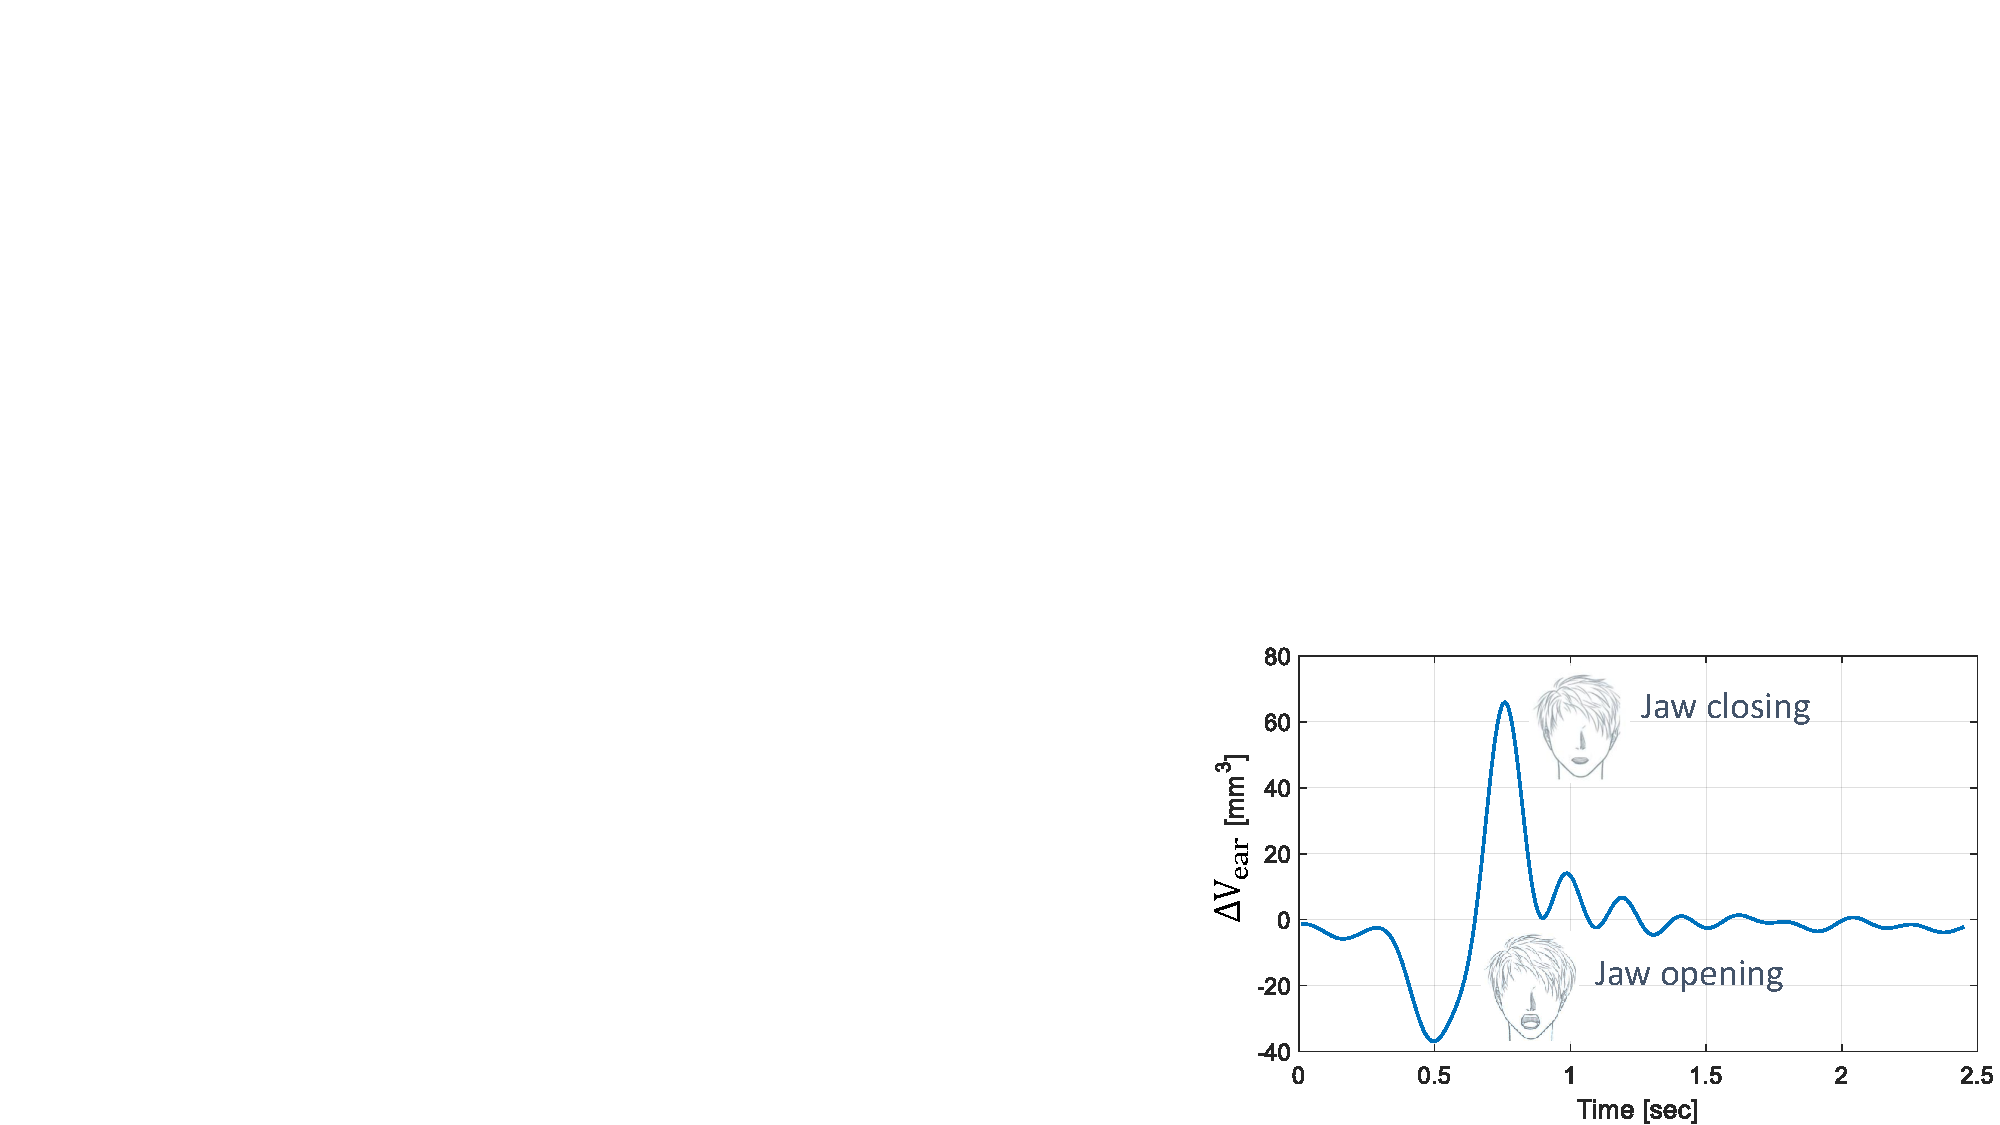
\includegraphics[trim={20.5cm 0cm 0cm 10.8cm},clip, width=0.4\textwidth]{figures/deltaV_ear.pdf}
	\caption{Ear canal volume variation for one mastication cycle}
	\label{fig:deltaV_ear}
\end{figure}
%%%%%%%%%%%%%%%%%%%%%%%%%%%%%%%%%%%%%%

The earplug operation characteristic behavior has not been studied yet. Thus, the evolution of the volume variation $\Delta V_{ear}$ is not well known as a function of the pressure variation $\Delta p_{ear}$. Then, considering the pressure and volume variation levels from \cite{Delnavaz2012} and \cite{Bouchard-Roy2020}, the equation \ref{eq:max_hydraulic_energy} approximates an upper limit for the extractable hydraulic energy with the maximum values of $\Delta p_{ear}$ et $\Delta V_{ear}$ that have been recorded, i.e. $p_c=12kPa$ and $\Delta V_{ear,m}=60$mm$^3$. $p_c$ stands for the comfort pressure by assuming that the user could feel discomfort if $\Delta p_{ear}>p_c$. The energy estimation presumes that the earplug is a perfect flow rate source, which is a theoretical hypothesis leading to $0.9$mJ available from one mastication. Based on 2200 mastication cycles per day, according to \cite{Goll2011}, there would be $2$mJ available per day, per ear. This amount of energy could theoretically enhance supply $23.5$\% of the $17$J of needed for the state of the art of cochlear implants \cite{Kulah2022}. Further research in both domains related to hearing aids and energy harvesting could lead to fully autonomous devices in the future.
\begin{align}
	\text{max}(E_{hyd}) = p_c \cdot \Delta V_{ear,m} = 0.9\text{mJ}
	\label{eq:max_hydraulic_energy}
\end{align}

    %///////////////////////////////////////////// 
	\subsection{The harvesting strategy}	
	\label{The harvesting strategy}
    %/////////////////////////////////////////////
Electromagnetic transducers are usually used to harvest energy from kinetic (vibration) energy sources. In fact, the power density of electromagnetic transducers decreases as much as the effective volume of transducing material and the frequency of the energy source decrease \cite{Priya2017,Kulah2008}. Also, the fabrication and the integration of the coil and the moving magnet can come out to be difficult as the gap between the two components has to be carefully managed to prevent non-linear unpredicted responses \cite{Caruntu2001}. Thus, piezoelectric ceramics appear like good candidates, but they can not be easily used because of their high stiffness and their high resonance frequencies (>$1.57$Hz). Therefore, the harvesting system could benefit from a frequency-up conversion stage \cite{Ashraf2011,Peng2021} to increase the frequency of the energy source and so the energy conversion efficiency of piezoelectric ceramic transducers. A majority of the frequency-up systems with piezoelectric transducers use mechanical stops with piezoelectric ceramic cantilevers to reach high frequencies with a good mechanical coupling \cite{Edwards2013,Gu2011,Lee2007}. Stoppers however dissipate energy. Alternative solutions use mechanically bistable resonators (BR) to perform frequency-up \cite{Vocca2012}. Recent works led to the development and optimization of  bistable structures integrating stacked piezoelectric ceramics inside flextensional elastic structures \cite{Huguet2017}. They show enhanced performances due to high electromechanical coupling.

We can estimate the best choice maximizing the energy extraction from the hydraulic source. Figure \ref{fig:OB_vs_LINEAR} shows in blue the hydraulic behavior of the ideal flow rate source previously introduced with the upper limit values of pressure and volume variations. To be harvested, the energy has to be stored in a mechanical potential reservoir at first, to be then converted in electricity by the transducer. The hydraulic-mechanic interface can be a hydraulic cylinder. In this way, the best linear resonator can theoretically exploit/store a maximum of $50\%$ from the maximum available hydraulic energy ($\text{max}(E_{hyd})$). Furthermore, BR usually admit non-linear elastic behavior. For example, a BR governed by a Duffing equation is inherently capable of exploiting $65$\% from the same energy source, which is $15$\% better than the best theoretical linear option.
%%%%%%%%%%%%%%%%%%%%%%%%%%%%%%%%%%%%%%
\begin{figure}[!htbp]
	\centering
	\captionsetup{justification=centering}
	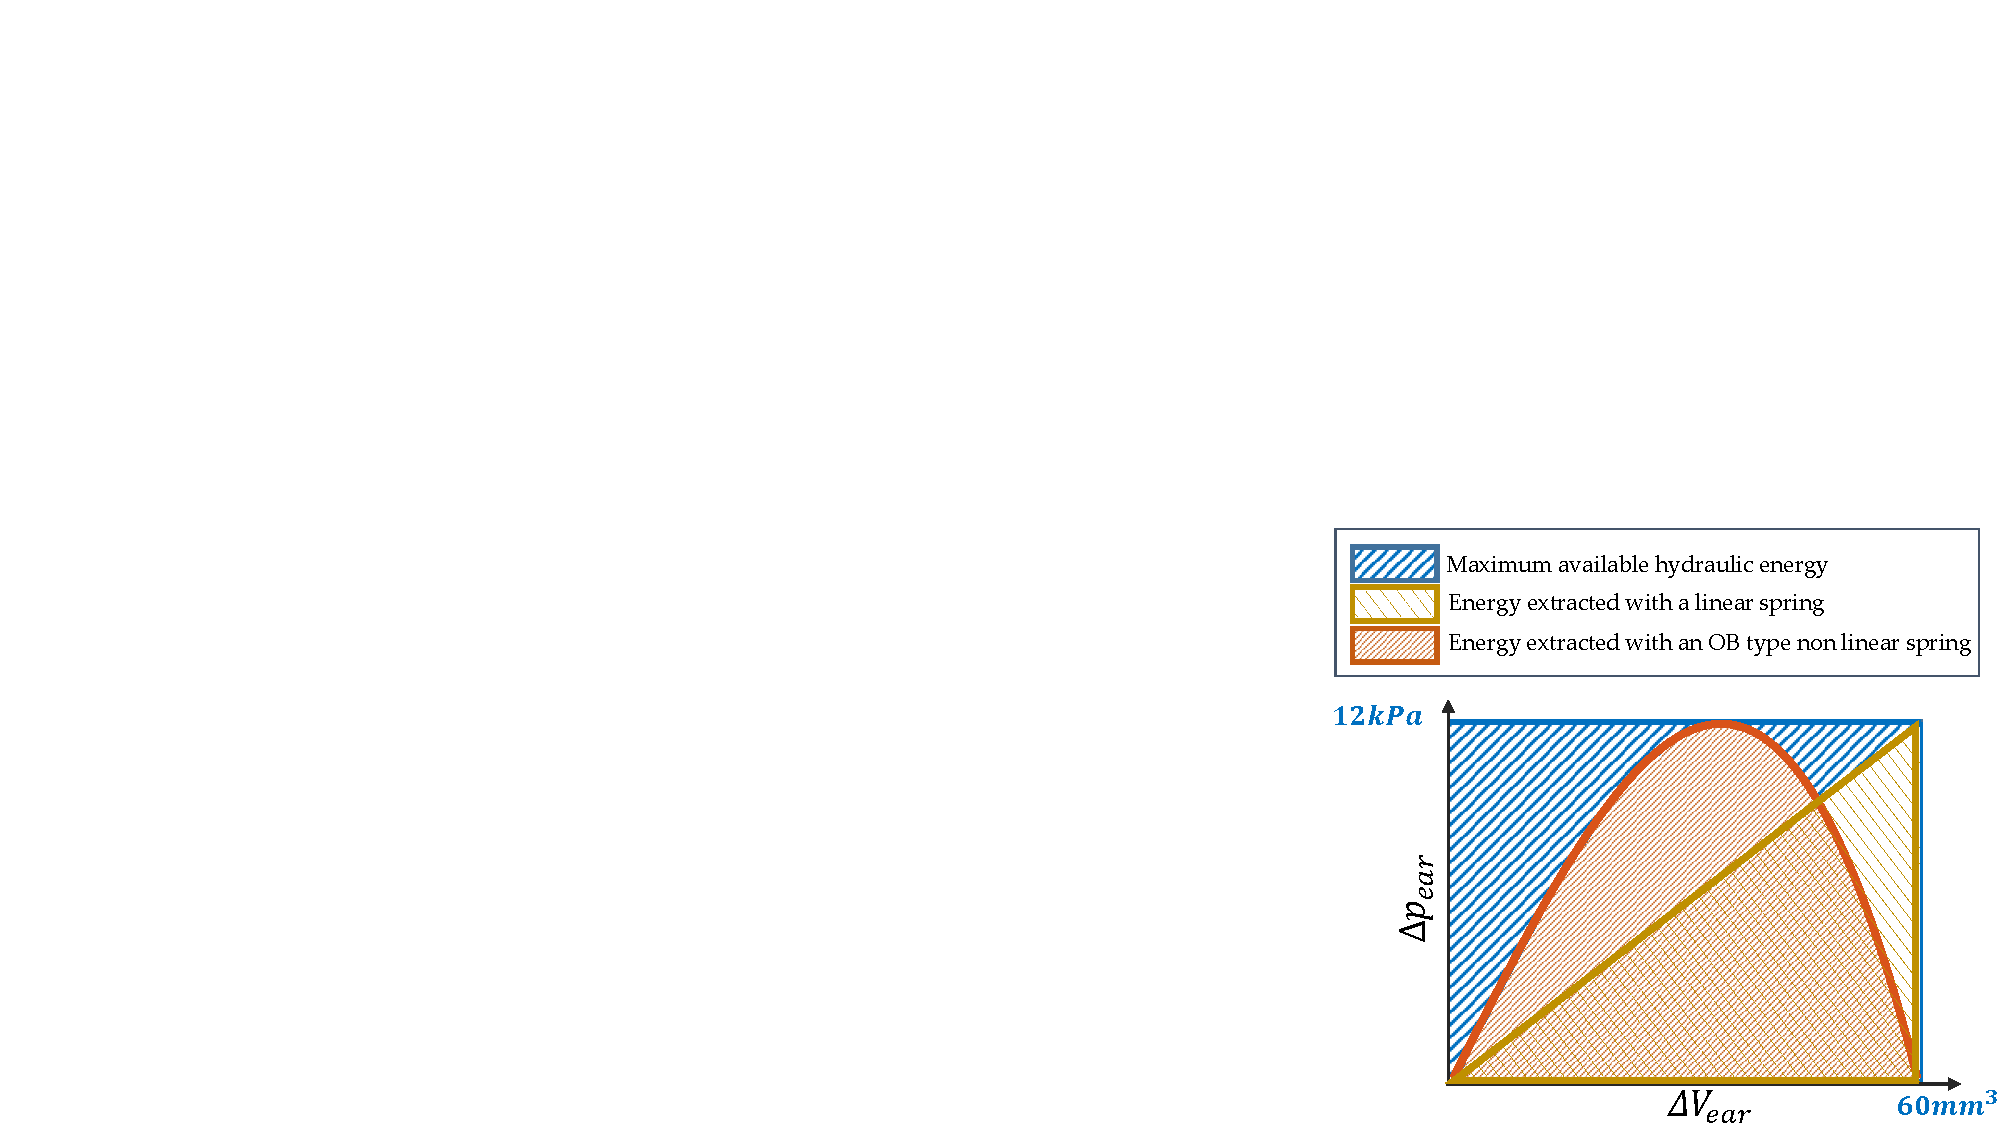
\includegraphics[trim={22.5cm 0cm 0cm 8.8cm},clip, width=0.35\textwidth]{figures/OB_vs_LINEAR.pdf}
	\caption{Hydraulic source exploitation depending on the mechanical load}
	\label{fig:OB_vs_LINEAR}
\end{figure}
%%%%%%%%%%%%%%%%%%%%%%%%%%%%%%%%%%%%%%
Hence, the absence of rubbing parts and the optimal energy extraction shed light on a BR as a promising solution for our application. 
%/!\/!\/!\/!\/!\/!\/!\/!\/!\/!\/!\/!\/!\/!\/!\/!\/!\/!\/!\/!\/!\/!\/!\/!\%
\section{HARVESTER PRESENTATION AND OPERATION \mbox{PRINCIPLE}}
\label{sec:HARVESTER PRESENTATION AND OPERATION PRINCIPLE}
%/!\/!\/!\/!\/!\/!\/!\/!\/!\/!\/!\/!\/!\/!\/!\/!\/!\/!\/!\/!\/!\/!\/!\/!\%

%%%%%%%%%%%%%%%%%%%%%%%%%%%%%%%%%%%%%%%
\begin{figure*}[!htbp]
	\centering
	\captionsetup{justification=centering}
	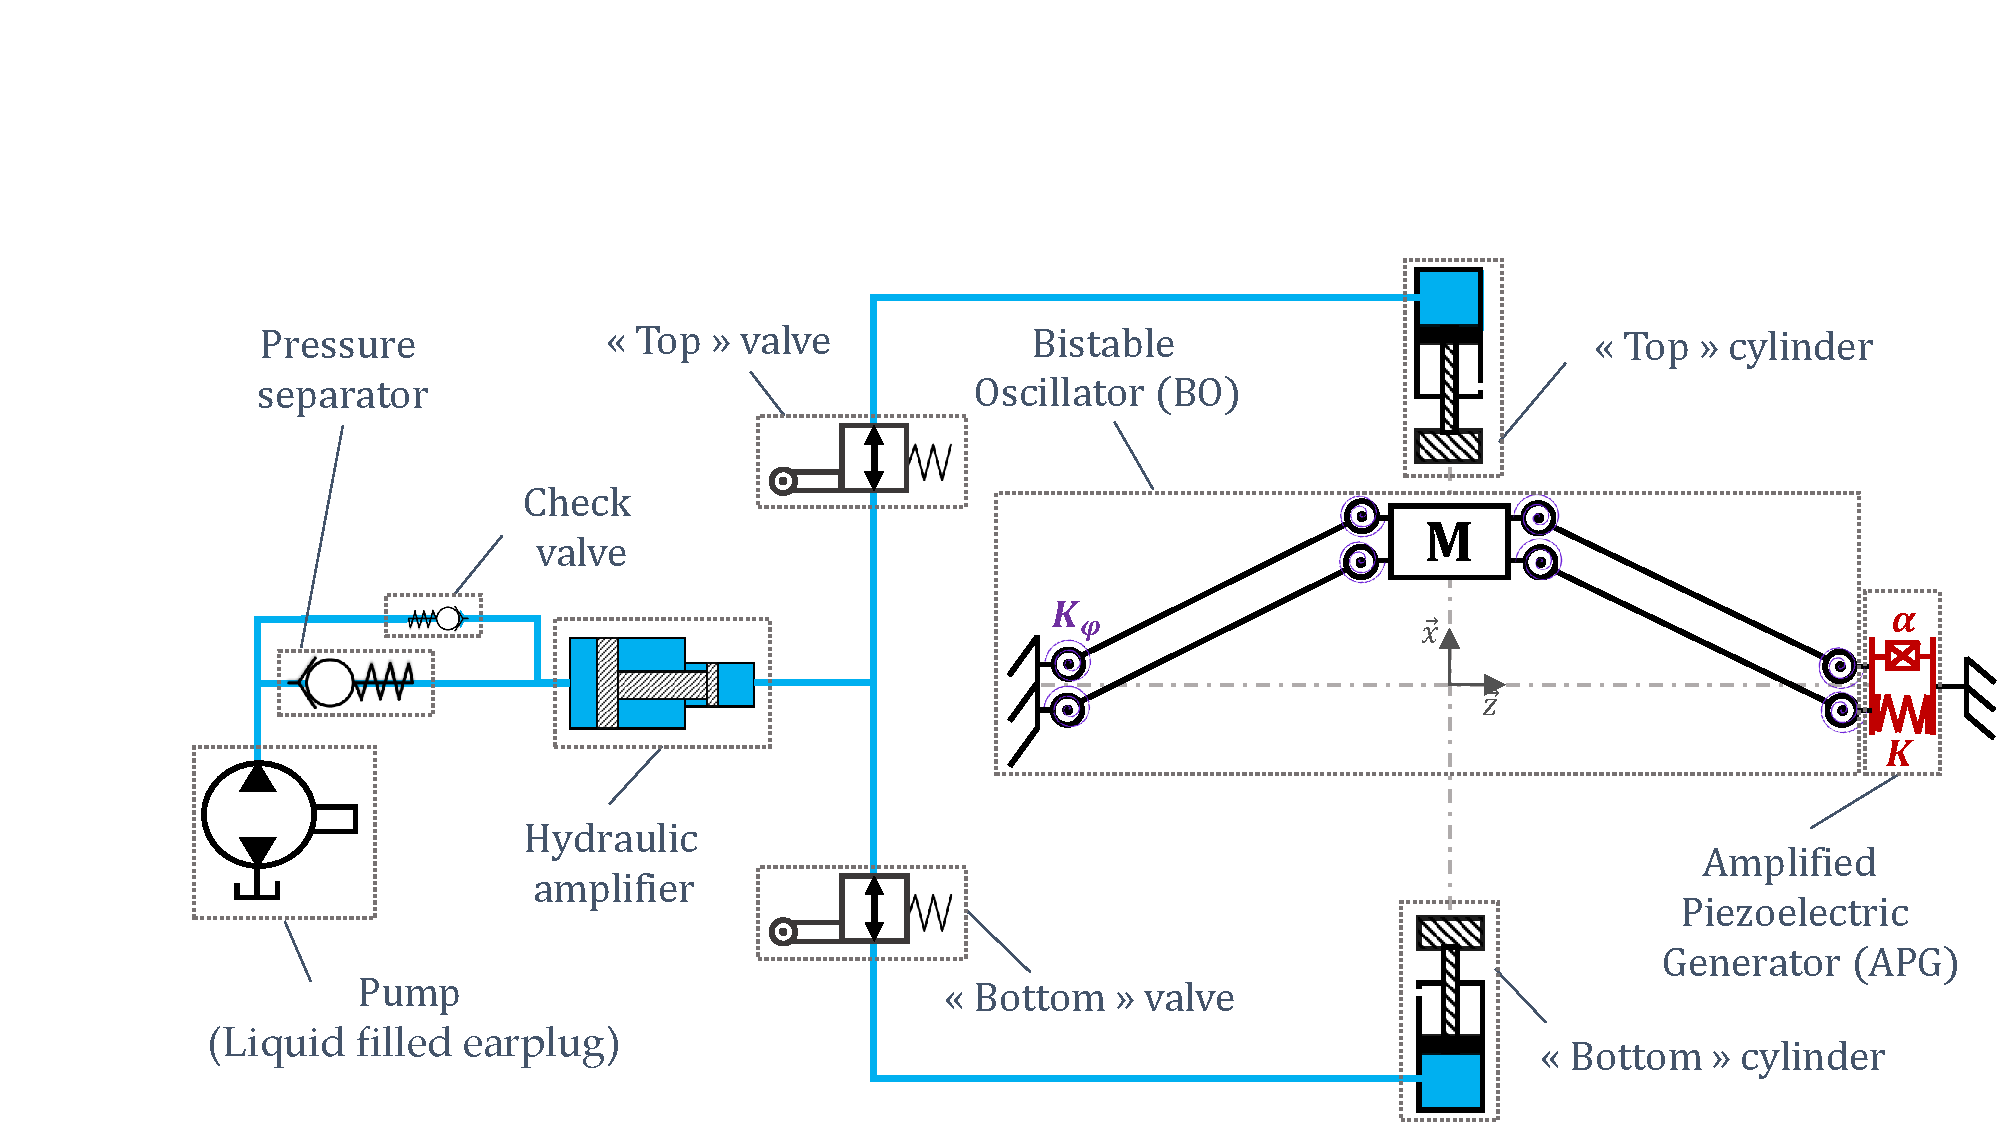
\includegraphics[trim={3.2cm 0cm 0cm 4.3cm},clip, width=0.7\textwidth]{figures/system_presentation.pdf}
	\caption{Schematic presentation of the frequency-up piezoelectric harvester exploiting the ear canal geometry variation} 
	\label{fig:system_presentation}
\end{figure*}
%%%%%%%%%%%%%%%%%%%%%%%%%%%%%%%%%%%%%%%
The figure \ref{fig:system_presentation} presents a schematic view of the energy harvesting system. It uses a liquid filled earplug to transmit the energy outside the ear canal and benefit so from larger effective space. To maximize the efficiency, the system integrates a frequency-up conversion stage performed by a bistable resonator (BR). The latter implements an amplified piezoelectric generator (APG) made of a flextensional elastic APX4 steel structure containing stacked lead zirconate titanate (PZT) ceramics (fig. \ref{fig:APG}). The electromechanical converter composed of the BR and the APG theoretically offers higher energy conversion efficiency compared to low frequency solutions and/or flexible electromechanical transducers \cite{Guo2019}.
%%%%%%%%%%%%%%%%%%%%%%%%%%%%%%%%%%%%	
\begin{figure}[!htb]
	\begin{center}
		\begin{subfigure}[t]{0.6\linewidth}
			\captionsetup{justification=centering}
			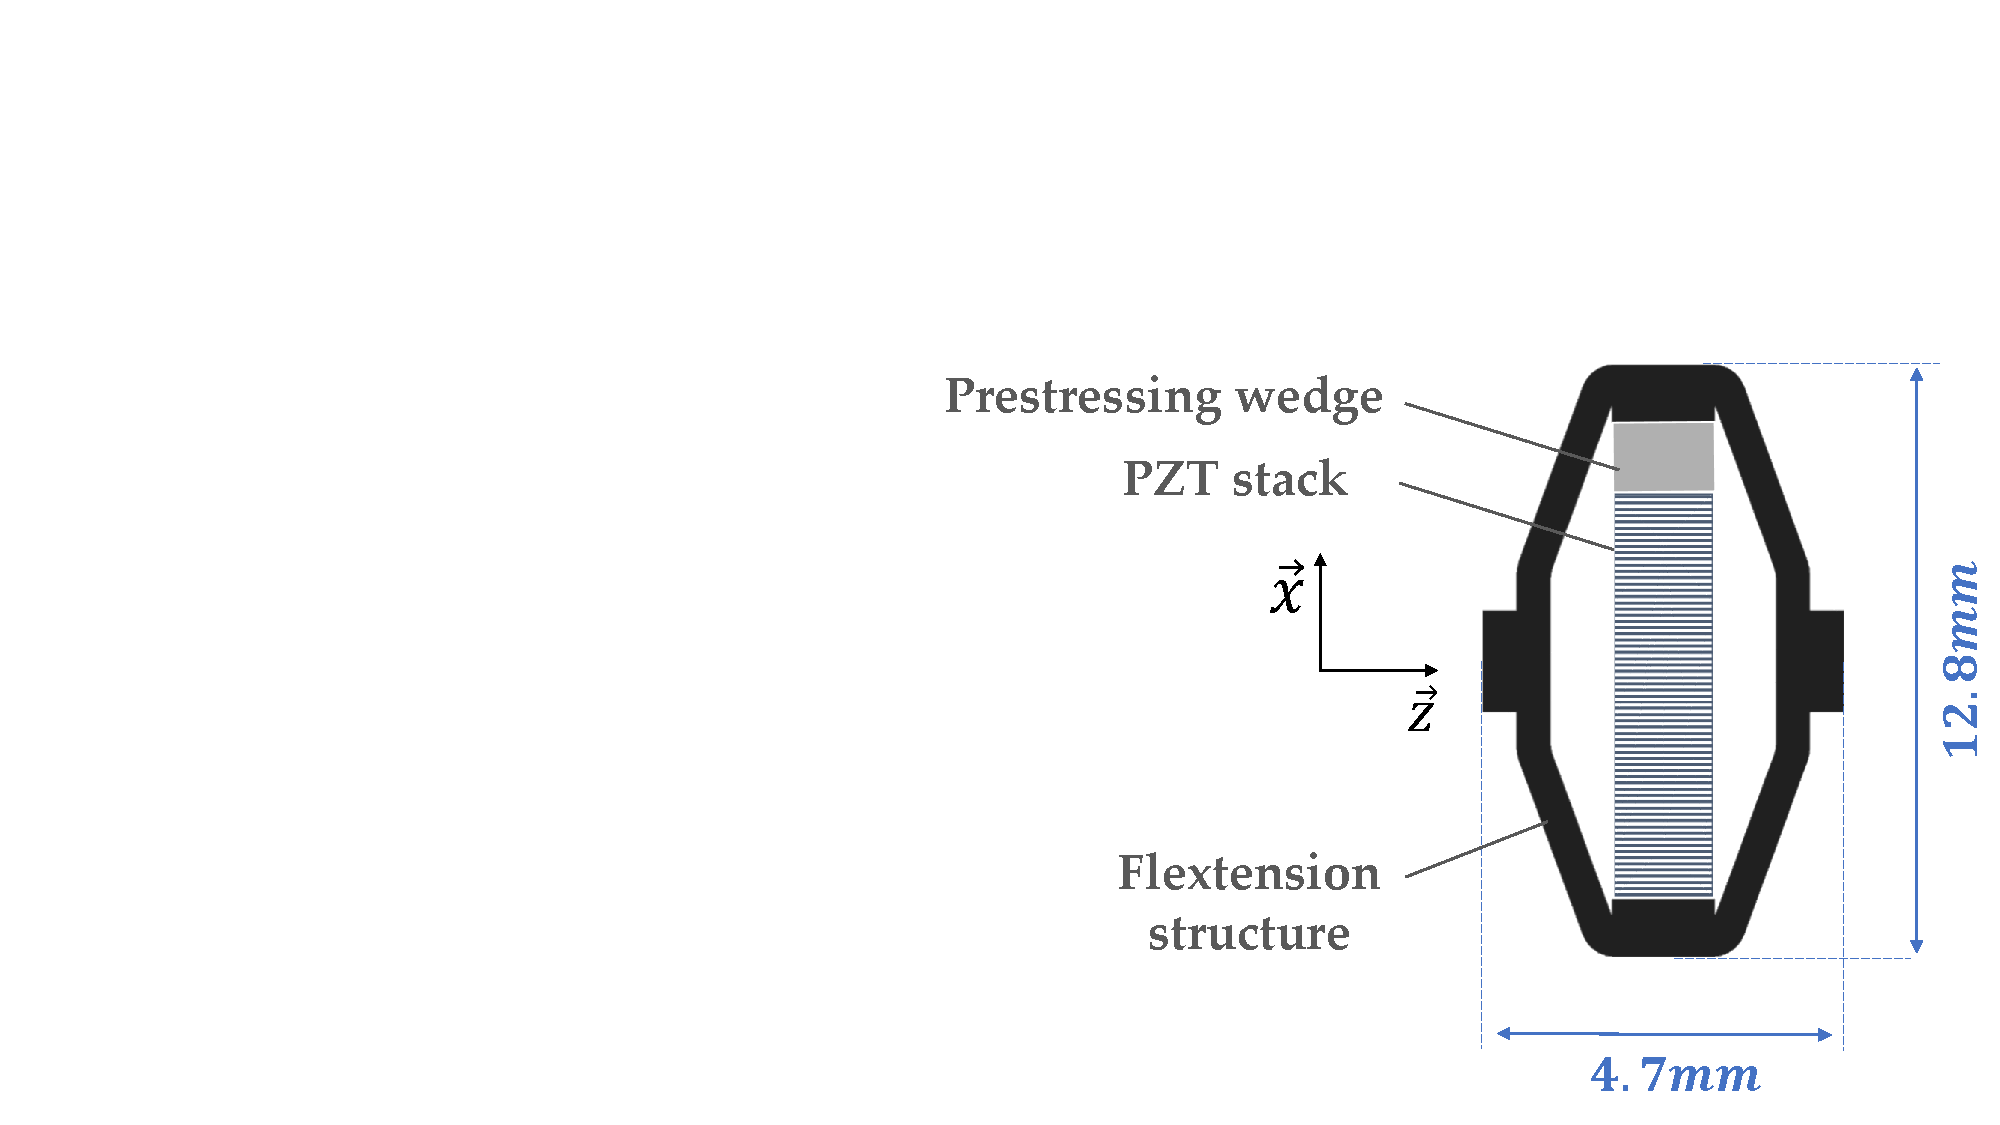
\includegraphics[trim={16cm 0cm 0cm 6cm},clip,width=\linewidth]{figures/APG_schema.pdf}
			\caption{Detailed schema}
			\label{fig:APG_schema}
		\end{subfigure}
		\hfillx
		\begin{subfigure}[t]{0.29\linewidth}
			\captionsetup{justification=centering}
			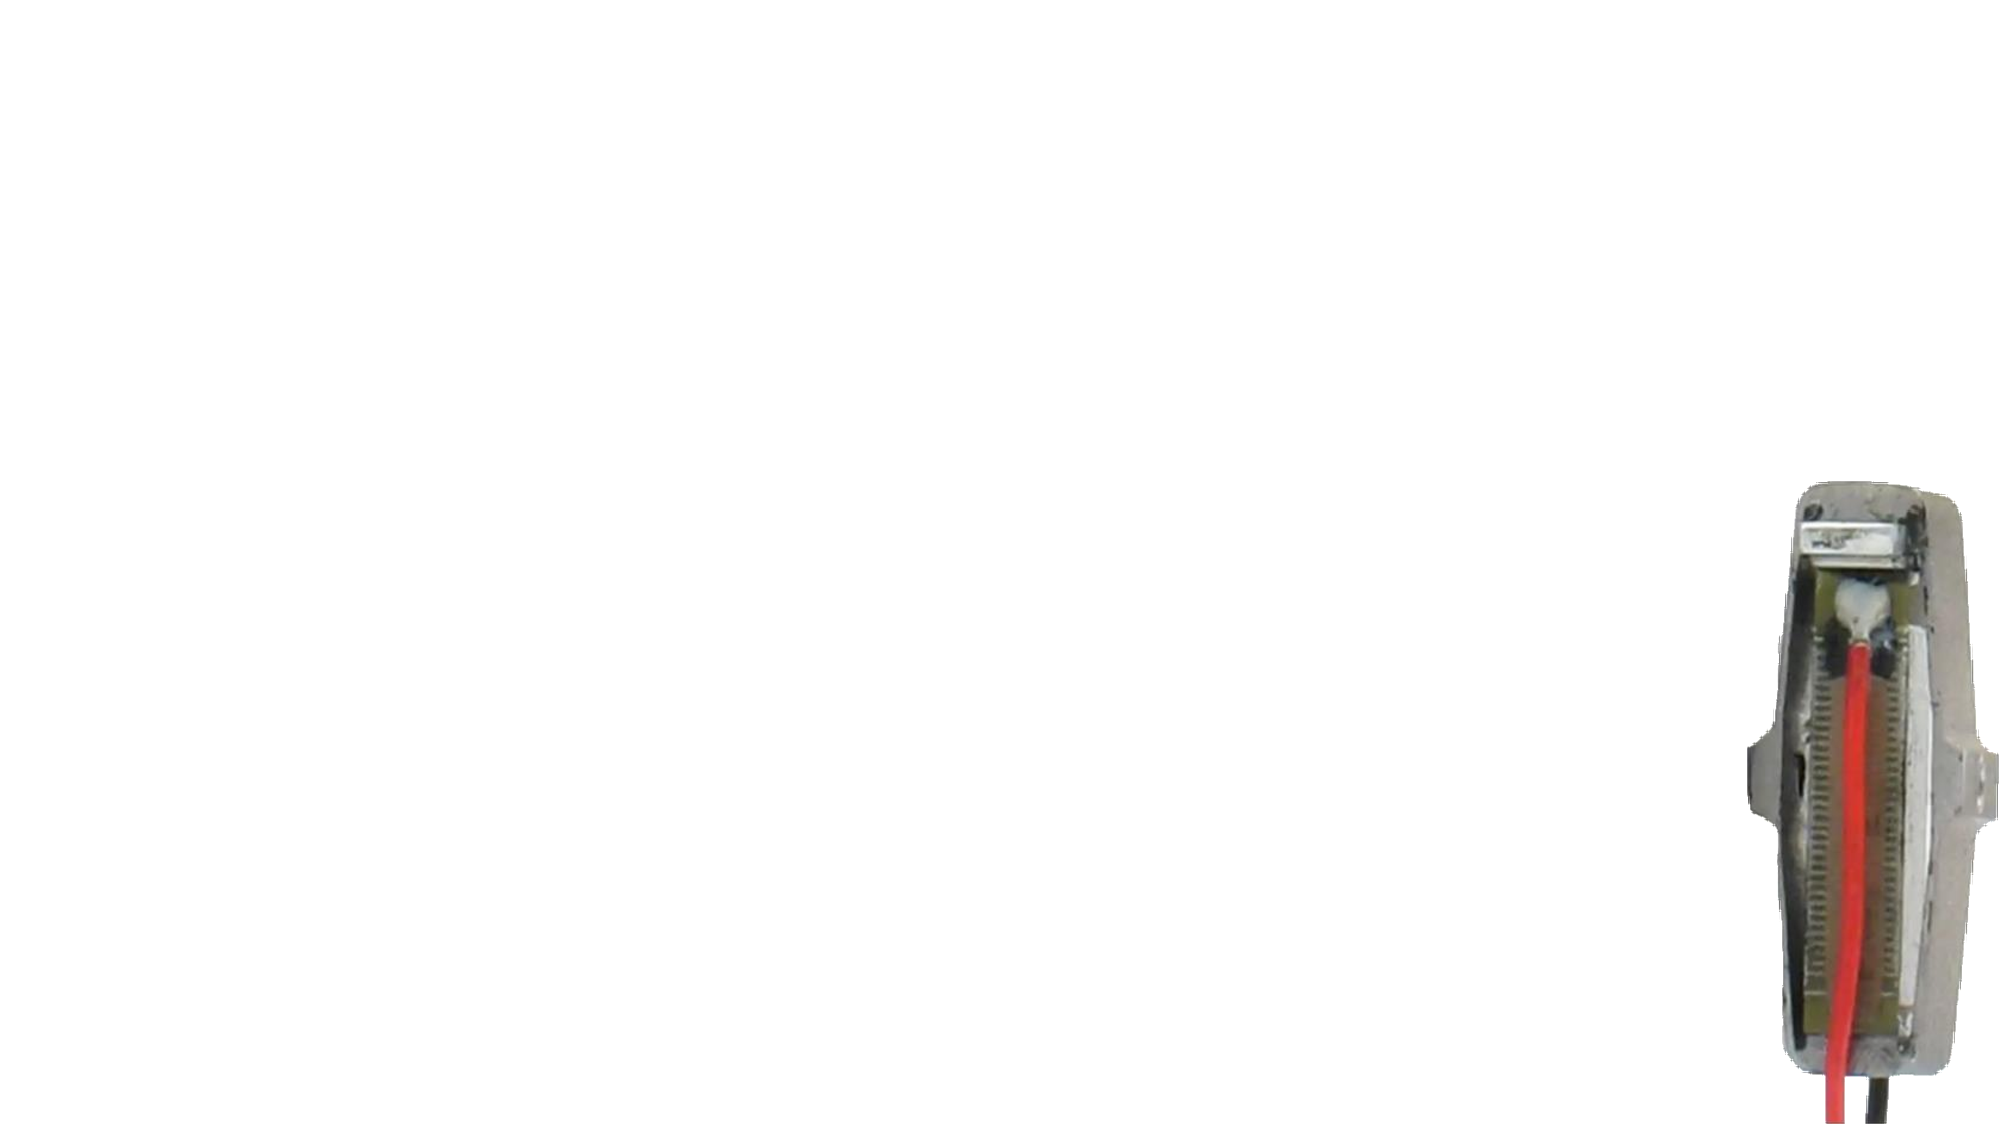
\includegraphics[trim={29.5cm 0cm 0cm 8cm},clip,width=0.65\linewidth]{figures/APG_photo.pdf}
			\caption{Picture}
			\label{fig:APG_photo}
		\end{subfigure}
		\caption{The APG presentation}
		\label{fig:APG}
	\end{center}
\end{figure}
%%%%%%%%%%%%%%%%%%%%%%%%%%%%%%%%%%%% 

The electromechanical converter is actuated, by two hydraulic cylinders (HC), with the hydraulic energy transmitted from the liquid filled earplug, through a pressure separator, a hydraulic amplifier and two hydraulic valves (HV).

To maximize the mechanical energy transfer between the ear canal and the earplug, the latter is lightly pressurized. A minimum of 14kPa is needed in order to fit the earplug to the ear canal wall \cite{Delnavaz2013}. The pressure separator ensures that this initial pressurization does not interfere on the system operation. Then, during a mastication cycle, the TMJ compresses the ear canal wall and expels so the fluid outside the earplug. The HVs ensure to led the fluid alternatively to each HC in order to actuate the BR mass back and forward. The hydraulic amplifier adapts the cylinders stroke to the available earplug flow rate and also adapts the mechanical impedance of the BR to the mechanical impedance of the ear canal wall.

The BR mass has two stable equilibrium positions, $x_m = x_0$ and $x_m = -x_0$. The harvester operates on two major phases. The first consists on the BR mass actuation, by a HC, from one stable equilibrium position toward the unstable position at $x_m = 0$. During the second phase the mass goes oscillate around the opposite stable equilibrium position until it stops, while a portion of the resonatory energy is converted in electricity by the GPA. The mass then moves backward during the next mastication, completing so the harvester cycle.
%%%%%%%%%%%%%%%%%%%%%%%%%%%%%%%%%%%%%%%
\begin{figure}[!htbp]
	\centering
	\captionsetup{justification=centering}
	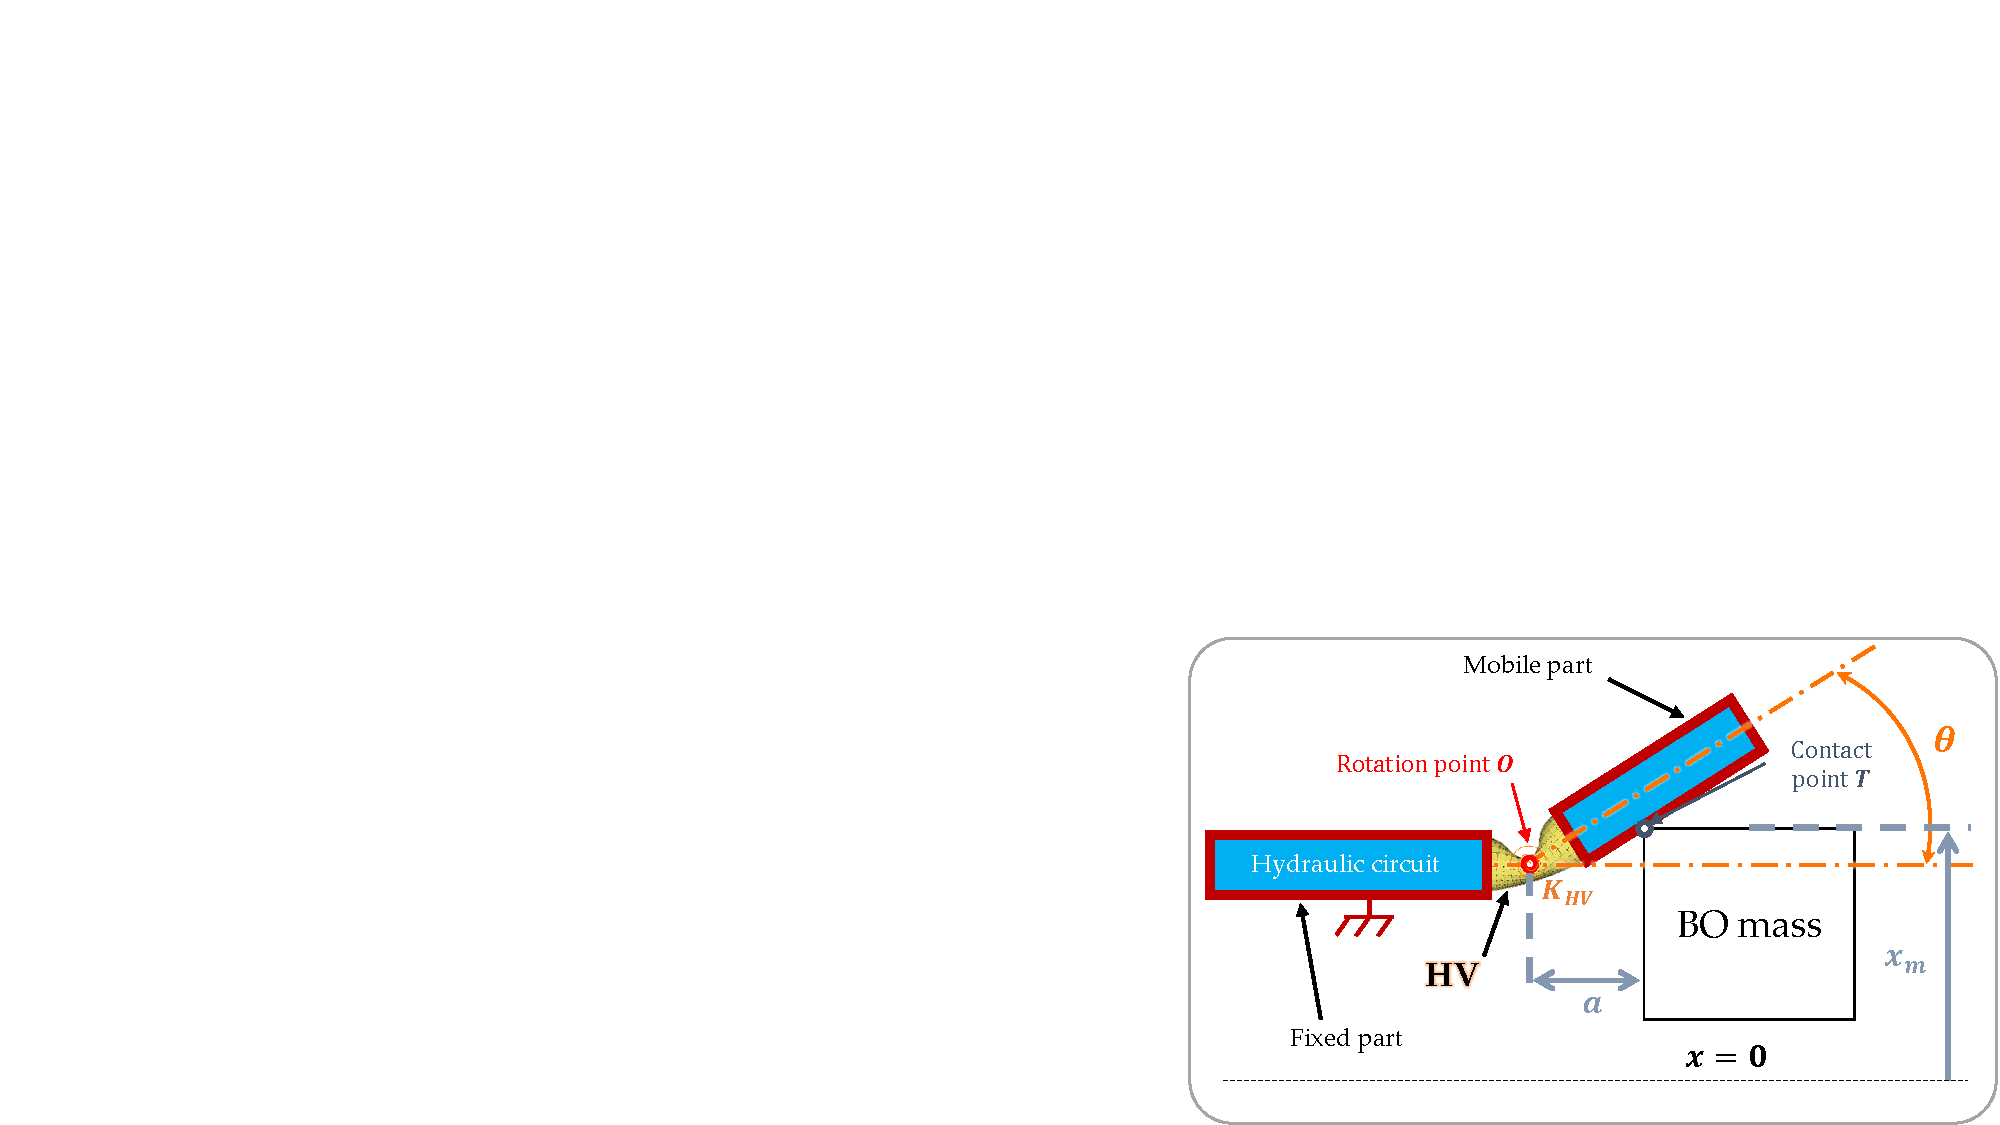
\includegraphics[trim={20cm 0cm 0cm 10.75cm},clip, width=\linewidth]{figures/HV_actuation_detail.pdf}
	\caption{Contact detail between a HV and the BR mass} 
	\label{fig:HV_actuation_detail}
\end{figure}
%%%%%%%%%%%%%%%%%%%%%%%%%%%%%%%%%%%%%%%

In order to maximize the harvested energy we must minimize the energy consumed by the HVs. A technological solution for this role is to use a flexible tube buckled by bending. The figure \ref{fig:HV_actuation_detail} schematizes the integration of such HV around the BR environment. The valve is composed of a flexible tube connected between a rigid part of the hydraulic circuit and a fixed one. The BR mass motion on the mobile part induces a bending angle $\theta$ around the rotational point $O$ located at the buckled section of the flexible tube. Consequently, a pressure loss is generated through the valve in buckled position. Thus, a HV is considered closed when the BR mass is at a stable equilibrium position ($x_m=\pm x_0$) and opened when the mass is at $x_m=0$. Two HVs symmetrically placed on each side of the $\vec{x}$ axis set up an opened hydraulic circuit on one side and a closed one on the other side, depending on the BR mass position. The HV technological choice is motivated by three major arguments. First, the absence of electromechanical transduction minimizes the energy losses for the valve operation. Then, the post-buckling softening of the bent tube minimizes the mechanical impact on the BR mass dynamic operation. Finally, it is well adapted at the millimetric application scale.

%/!\/!\/!\/!\/!\/!\/!\/!\/!\/!\/!\/!\/!\/!\/!\/!\/!\/!\/!\/!\/!\/!\/!\/!\%
\section{SYSTEM GLOBAL MODELING}
\label{sec:SYSTEM MODELING}
%/!\/!\/!\/!\/!\/!\/!\/!\/!\/!\/!\/!\/!\/!\/!\/!\/!\/!\/!\/!\/!\/!\/!\/!\%
The harvester is a multyphisic system composed of hydraulic, mechanical, and electrical components. This section presents a global multiphysic model describing the theoretical system operation. Two coupled subsystems are considered. The subsection \ref{subsec:The electromechanical converter} shows the modeling of the electromechanical frequency-up converter (BR + APG) under the mechanical influence of a HV and a HC. Then, the subsection \ref{subsec:The hydraulic circuit} discusses the design of the hydraulic circuit composed of the two HVs, the two HCs, the hydraulic amplifier, the pressure separator and the liquid filled earplug. Finally, the section \ref{subsec:Global model simulation} exposes the numerical simulation of the designed multiphysic coupled model.

    %///////////////////////////////////////////// 
	\subsection{Modeling of the electromechanical converter}	
	\label{subsec:The electromechanical converter}
    %/////////////////////////////////////////////
%%%%%%%%%%%%%%%%%%%%%%%%%%%%%%%%%%%%%%
\begin{figure*}[!htbp]
	\centering
	\captionsetup{justification=centering}
	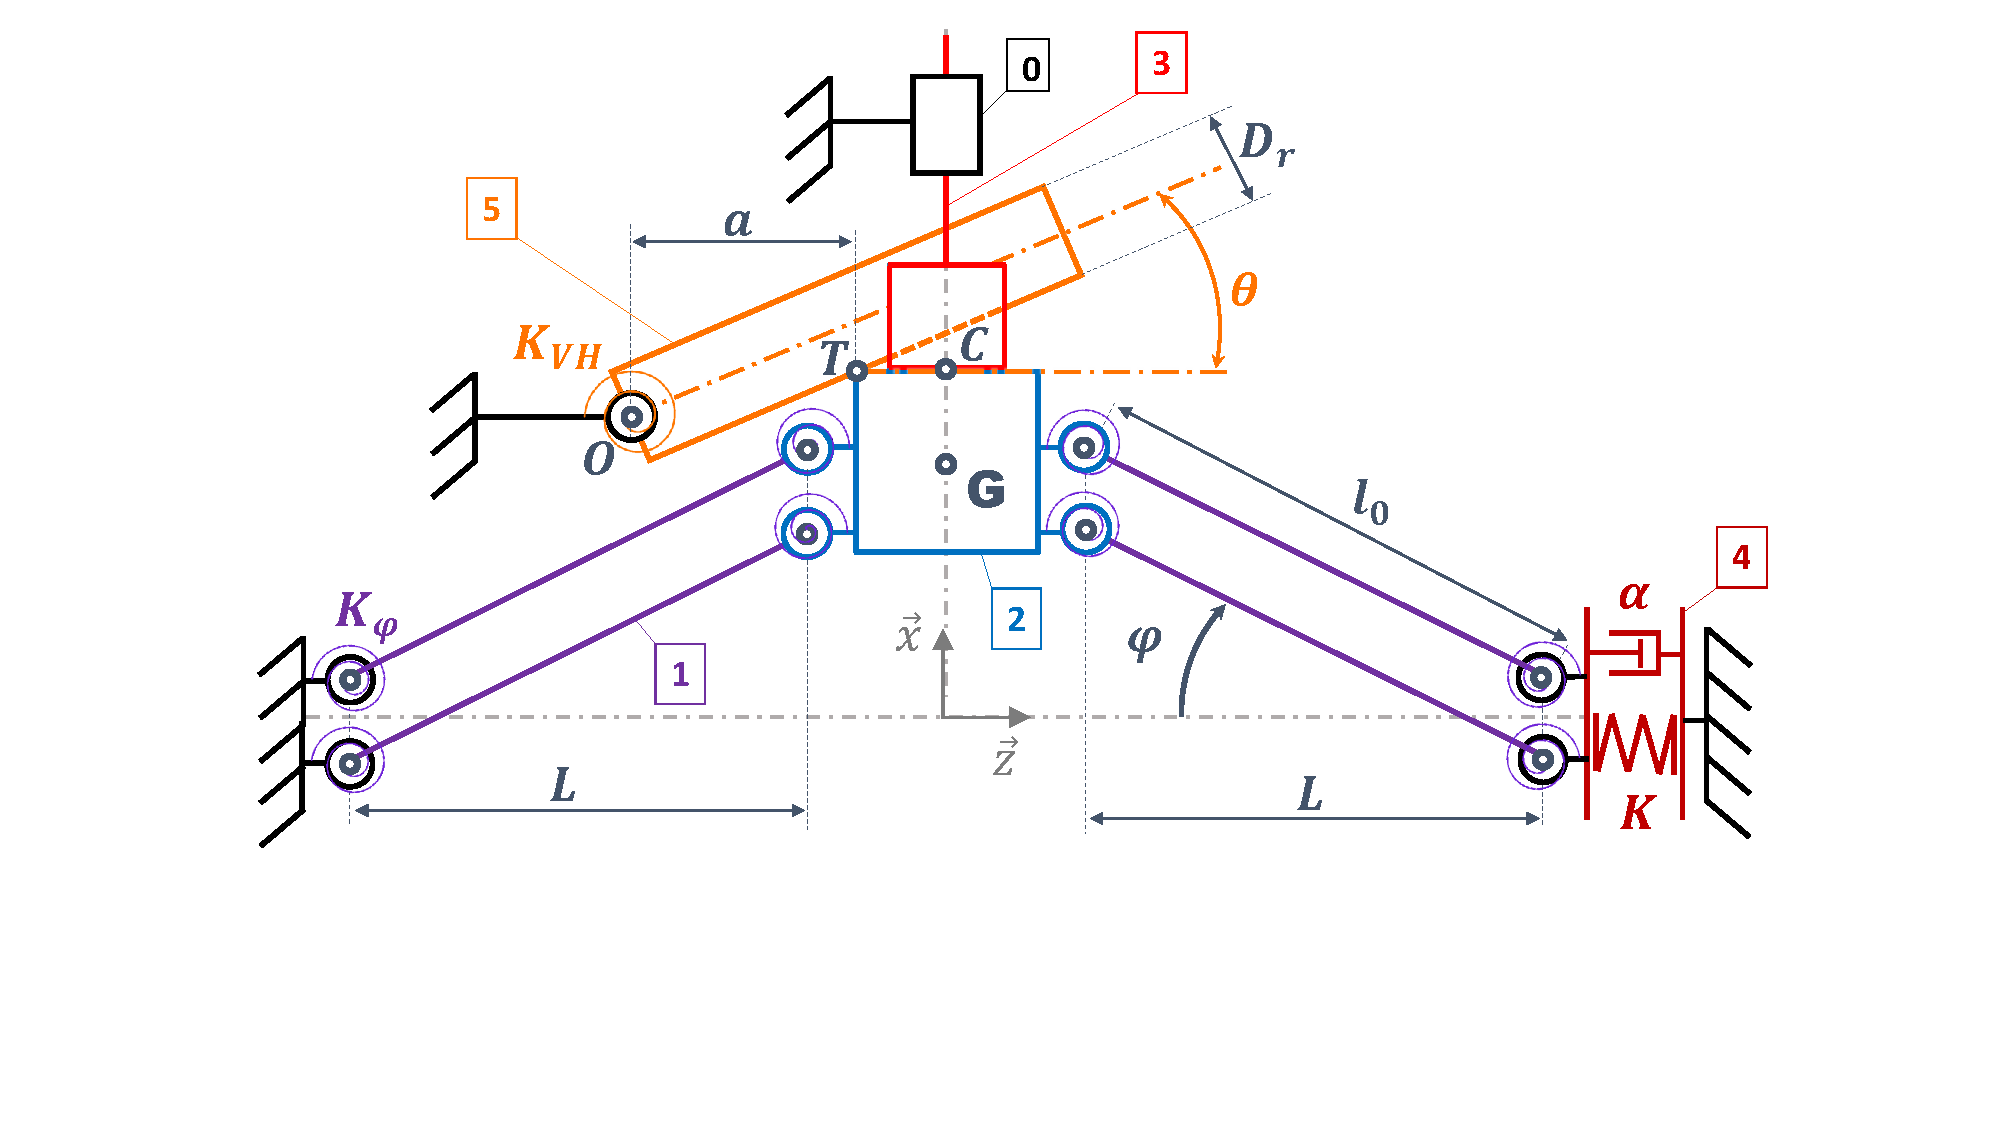
\includegraphics[trim={0cm 0cm 0cm 0cm},clip, width=0.9\textwidth]{figures/schema_cinematique1.pdf}
	\caption{Cinematic schema of the of the electromechanical converter under the mechanical influence of a HV and a HC}
	\label{fig:schema_cinematique1}
\end{figure*}
%%%%%%%%%%%%%%%%%%%%%%%%%%%%%%%%%%%%%%

The figure \ref{fig:schema_cinematique1} shows the cinematic schema of the electromechanical converter under the mechanical influence of a HV and a HC. The different schematized rigid bodies all designated in the table \ref{tab:Designation of rigid bodies}. The BR is represented by 4 identical arms articulated by 8 hinges and a central mass. The APG is considered as a spring of stiffness $K$ with an electromechanical coupling $k^2$, indicative of the piezoelectric transduction, expressed by the equation \ref{eq:k2_def}.\\
The model is based on the following hypotheses:
\begin{itemize}
	\item The only mass considered is the BR mass (2).
	\item All parts are infinitely rigid beside the APG (4).
	\item The hinges are considered elastic. They are defined by their rotational stiffness $K_{\varphi}$ and their mechanical damping is included in the global viscous damping coefficient $\mu$.
	\item The contact between the BR mass (2) and the HC piston head (5) is considered permanent.
	\item We assume the small-angle approximation with \mbox{$x_0<<L$}. 
\end{itemize}
\begin{equation}
	k^2 = \dfrac{\alpha^2}{\alpha^2 +  K C_p}
	\label{eq:k2_def}
\end{equation}
%%%%%%%%%%%%%%%%%
\begin{table}[!htbp]
\centering
	\begin{tabular}{ c | c }
		\toprule
		\multicolumn{1}{c}{\textbf{Num}}  &
		\multicolumn{1}{c}{\textbf{Name}}  \\
		\midrule
		0	& Fixed frame      	  	\\  
		1	& BR arm      	  	\\  
		2	& BR mass     	\\
		3	& HC piston head	\\
		4	& APG     	\\
		5	& Simplified HV mechanical model     	\\
		\bottomrule
	\end{tabular}
	\caption{Designation of rigid bodies}
\label{tab:Designation of rigid bodies}
\end{table} 
%%%%%%%%%%%%%%%%%%%%%  

By isolating the BR mass and using the Newtons 2$^{nd}$ law, we can express its dynamic equilibrium with respect to the different external forces. The projection on the $\vec{x}$ axis of the resulting expression is given by the equation \ref{eq:OB-GPA} where the provenance of the different terms is highlighted. The BR mechanical equilibrium took aside contains the mass inertial term, a non-linear stiffness depending on $x_m$, the hinges stiffness and viscous losses. This expression has also been demonstrated by the Lagrange method in past works \cite{Liu2013}. The first term introduced by the HV is related to its rotationnal stiffness and the second term is related to the friction losses at the contact point $T$ (fig. \ref{fig:HV_actuation_detail}). A dry friction model is choose to describe the nature of the contact between the two components. Thus, $F_f$ will depend on a dry friction coefficient $\mu_f$, related to the nature of the material that are rubbing, and the sign of $\dot{x}_m$ (eq. \ref{eq:Dry_friction}). The force $F_{pis}$ induced by the piston head of the HC on the OB mass will depend on hydraulic parameters. The hydro-mechanical coupling is highlighted later by the equation \ref{eq:equilibre_dynamique_piston_ouvert}.
\begin{equation}
	F_f = \mu_f \text{sign}(\dot{x}_m)
	\label{eq:Dry_friction}
\end{equation}

The electrical power generated by the APG is dissipated in a load resistor $R_{ch}$ calculated with an adaptive impedance matching expressed by the equation \ref{eq:R_ch_adaptive_imp} \cite{Liu2013}. 
\begin{equation}
	R_{ch} = \dfrac{1}{C_p w_0}
	\label{eq:R_ch_adaptive_imp}
\end{equation}
Thus, the equation governing the electrical behavior of the APG is :
\begin{equation}
	\dfrac{U_p}{R_{ch}} = 
	-\alpha\dfrac{d}{dt}\biggl(2\sqrt{{l_0}^2-x_m^2}\biggr)
	- C_p\dot{U_p}
	= \frac{2\alpha x_m\dot{x}_m}{\sqrt{L^2+x_m^2}} - C_p\dot{U_p}
\end{equation}
Consequently, the generated power $P_e$ expression is :
\begin{equation}
	P_e = \frac{{U_p}^2}{R_{ch}} 
	\label{eq:P_e}
\end{equation} 
With the small-angle approximation, the system equation \ref{eq:OB+GPA+VH+piston} defines the electromechanical behavior of the harvester. The HV stiffness $K_{HV}$ will depend on its bending angle $\theta$ and the latter will geometrically depend on the BR mass position $x_m$, as showed in figure \ref{fig:HV_actuation_detail}.

%%%%%%%%%%%%%%%%%%%%%%%
\begin{figure*}
\begin{equation}
\overbrace{\ m \ddot{x}_m =-2K(\sqrt{x_m^2+L^2}-l_0)\tan(\varphi) 
							-\mu \dot{x}_m
							-\frac{4K_{\varphi}\varphi}{L}\ }^{OB}
			\underbrace{\ -2\alpha U_p \tan(\varphi)\ }_{APG}		 
			\overbrace{\ -\dfrac{K_{HV}\theta}{a} - F_f\ }^{HV}
			\underbrace{\ -F_{pis}\ }_{HC}
\label{eq:OB-GPA}
\end{equation}
\end{figure*}
% \FloatBarrier
%%%%%%%%%%%%%%%%%%%%%%%
%%%%%%%%%%%%%%%%%%%%%%%
\begin{figure*}
\begin{equation}
% \begin{small}
	\begin{dcases}
\ddot{x}_m = - \frac{2K{x_0}^2}{mL^2}\biggl(\frac{x_m^2}{{x_0}^2} -1\biggr)
			   x_m - \frac{\mu}{m}\dot{x}_m - \frac{2\alpha U_p\ x_m}{mL}
			-\frac{K_{VH}(x_m)\theta(x_m)}{ma}
			-\frac{F_f}{m}
			-\frac{F_{pis}}{m} \\
\dfrac{U_p}{R_{ch}} = \frac{2\alpha x_m \dot{x}_m}{L} - C_p\dot{U}_p
	\end{dcases}
	\label{eq:OB+GPA+VH+piston}	
% \end{small}
\end{equation}
\end{figure*}
% \FloatBarrier
%%%%%%%%%%%%%%%%%%%%%%%
    %///////////////////////////////////////////// 
	\subsection{Modeling of the hydraulic circuit}	
	\label{subsec:The hydraulic circuit}
    %/////////////////////////////////////////////
This work challenges are focused on the experimental validation of the electromechanical converter cycled by two hydraulic valves. In fact several hydraulic miniature solutions are introduced by the literature for both of the components \cite{Wang2020,Xu2021,Zhu2013}. Hence, this section neglects the pressure loss through the pressure separator and the energy loss inside the hydraulic amplifier. These hydraulic components will rather be considered on further work.

In order to model the coupled behavior of the two hydraulic branches, we will use the index "$o$" for the open branch and the index "$c$" for the closed one. The following hypotheses will be considered :
\begin{itemize}
	\item The fluid is incompressible and Newtonian.
	\item The hydraulic circuit is non-deformable (no volume change) and there is no leakage.
	\item The hydraulic actuation is considered quasi-static (QS) in front
	the oscillation frequency of the BR.
\end{itemize}
The projection on the $\vec{x}$ axis of the Newtons 2$^{nd}$ law applied respectively to each HC moving piston gives us their mechanical equilibrium as follows :
\begin{align}
	\text{Opened cylinder ~}& \left\{~
	-F_{pis} - p_{oc}\ S_{c} - \lambda_{c}\ \dot{x}_{oc} = 0
	\right.
	\label{eq:equilibre_dynamique_piston_ouvert}\\
	\text{Closed cylinder ~}& \left\{~
	p_{cc}\ S_{c} - \lambda_{c}\ \dot{x}_{cc} = 0
	\right.
	\label{eq:equilibre_dynamique_piston_ferme}
\end{align}
Where $p_c$ is the HC chamber pressure and $x_c$ its moving piston position. $F_{pis}$ accounts for the OB counter-reaction on the HC. Thus, with the QS assumption, it can be derived from equation \ref{eq:OB+GPA+VH+piston} and expressed as follows : 
\begin{align}
	-F_{pis} & = F_{br}\\
	-F_{pis} & = -\frac{K\ {x_0}^2}{L^2}\biggl(\frac{x_m^2}{{x_0}^2} -1\biggr)x_m - \biggl( \frac{K_{HV}\theta}{a} \biggr) - F_f
	\label{eq:F_OB_xxxxxx}
\end{align}
Then, by juxtaposing the Bernoulli's equation for a current line, we can express the earplug inside pressure $p_{ear}$ as a function of the hydraulic resistance in the two parallel branches with the equations \ref{eq:Bernoulli_piston_ouvert} and \ref{eq:Bernoulli_piston_ferme}.
\begin{align}
	\text{Opened branch ~}& \left\{~
	p_{ear} = p_{in} + \dfrac{1}{a_h}\biggl(p_{oc} + Cf_0 {q_0}^2 \biggr)
	\right.
	\label{eq:Bernoulli_piston_ouvert}\\
	\text{Closed branch ~}& \left\{~
	p_{ear} = p_{in} + \dfrac{1}{a_h}\biggl(p_{cc} + Cf(x_m) {q_f}^2 \biggr)
	\right.
	\label{eq:Bernoulli_piston_ferme}
\end{align}
Where $p_{in}$ is the initial pressurization, $a_h$ is the hydraulic amplification ratio, $q$ the flow rate and $Cf$ the pressure loss coefficient of a HV. The latter will depend on the HV bending angle $\theta$ and therefore on the BR mass position $x_m$ (fig. \ref{fig:HV_actuation_detail}). $Cf$ will be as more important as the $x_m$ increases. It is minimal when the HV is unbent and worth $Cf_0$.

Also, the no leakage assumption imposes that all the outgoing fluid from the earplug is contained in the two hydraulic branches (eq. \ref{eq:conservation_masse}).
\begin{equation}
	q_{ear} = q_o + q_f
	\label{eq:conservation_masse}
\end{equation}
Moreover, the same previous hypothese requires that all the fluid entering the HC results on a piston displacement (eqs \ref{eq:conservation_masse_ouvert},\ref{eq:conservation_masse_ferme}).
\begin{align}
	\text{Opened cylinder ~}& \left\{~
	q_o = S_{hc} \dot{x}_{oc}
	\right.
	\label{eq:conservation_masse_ouvert}\\
	\text{Closed cylinder ~}& \left\{~
	q_c = S_{hc} \dot{x}_{cc}
	\right.
	\label{eq:conservation_masse_ferme}
\end{align}

    %///////////////////////////////////////////// 
	\subsection{Preliminary dimensioning}	
	\label{subsec:Preliminar dimensionning}
    %/////////////////////////////////////////////
The dimensioning starts by setting technological choices in order to experimentally validate the multiphysic coupled model. Therefore, the APG is a APA50XS piezoelectric actuator, from Cedrat Technologies, exploited as a generator, setting so the stiffness $K$. Then, the MQP4-10S HC from SMC will ensure the hydraulic to mechanical interface, setting then the cylinder piston section $S_{hc}$. Next, the hydraulic commutation of the two parallel branches is driven by two HVs made of collapsed flexible tubes, setting then $Cf(x_m)$. Finally, the \mbox{$L=16mm$ }parameter is chosen to be consistent with the application scale. 

The maximum energy extractable with the BR through a QS actuation is equal to the height of the potential energy barrier $E_{pb}$ when the mass position varies from \mbox{$x_m=\pm x_0$ }to \mbox{$x_m=0$}. Knowing that it is equal to 65\% of the upper limit of the available hydraulic energy (eq. \ref{eq:max_hydraulic_energy} $\&$ fig. \ref{fig:OB_vs_LINEAR}), we can set the BR buckling level \mbox{$\epsilon = x_0/L$} through the equation \ref{eq:Ep_bar}. The harvester is thus optimized depending on the energy source.
\begin{equation}
	E_{pb} = \dfrac{K x_0^4}{3L^2}=0.65p_c \Delta V_{ear,m}
	\label{eq:Ep_bar}
\end{equation}
Two additional coupled requirements allow the system operation by setting the amplification level $a_h$. First, the available fluid must be enough to ensure the HC stroke from its equilibrium position until the BR mass reaches \mbox{$x_m=0$} (eq. \ref{eq:contrainte_course}). Then, the BR mechanical impedance on $\vec{x}$ axis reaches a maximum value $F_c$ when \mbox{$ x_m = x_c = \dfrac{x_0}{\sqrt{3}}$}. At this point, a maximum pressure is induced in the earplug and so the equation \ref{eq:contrainte_confort} has to be verified to ensure the user comfort. If not, $\epsilon$ must be decreased, decreasing the extracted energy for the benefit of comfort.
\begin{empheq}[left=\empheqlbrace]{align} 
	\Delta V_{ear,m} = a_h\ S_{hc}\  x_{c0}
	\label{eq:contrainte_course}\\
	p_c > \frac{1}{a_h} \frac{F_c}{S_{hc}} ~~~~ \text{with}~~~~ F_c = \dfrac{4Kx_0^3}{3\sqrt{3}L^2}
	\label{eq:contrainte_confort}
\end{empheq}

%/!\/!\/!\/!\/!\/!\/!\/!\/!\/!\/!\/!\/!\/!\/!\/!\/!\/!\/!\/!\/!\/!\/!\/!\%
\section{NUMERICAL MODEL AND SIMULATIONS}
\label{NUMERICAL MODEL AND SIMULATIONS}
%/!\/!\/!\/!\/!\/!\/!\/!\/!\/!\/!\/!\/!\/!\/!\/!\/!\/!\/!\/!\/!\/!\/!\/!\%

	%///////////////////////////////////////////// 
	\subsection{Targeted hydraulic behavior of the HVs}	
	\label{subsec:HV hydraulic targeted behavior}
	%/////////////////////////////////////////////
A multiphysic coupled model has been established with the equations and the preliminary dimensioning previously introduced. The unknown key aspect stays the hydraulic behavior $Cf(x_m)$ of the HVs. The numerical resolution of the differential equations can provide the necessary condition to satisfy in order to perform the adequate hydraulic commutation. In fact, the ratio between the pressure loss coefficient of the closed HV and the one of the opened HV has to be sufficient to force the flow through the opened branch. So we introduce the hydraulic restriction coefficient $r_{Cf}$ defined as follows :
\begin{equation}
	r_{Cf} = \dfrac{Cf(\text{Closed HV})}{Cf(\text{Opened HV})}	= \dfrac{Cf_c}{Cf_0}	
	\label{eq:r_Cf_definition}
\end{equation}
Where $Cf_c=Cf(\pm x_0)$. The literature does not provide the constitutive relation between $x_m$ and $Cf$ for a buckled flexible tube. Therefore, we preliminarily assume that it is linear and defined as follows :
\begin{align}
	Cf(x_m) & = Cf_0 + \dfrac{Cf_c - Cf_0}{x_0}\ x_m  \notag \\
			& = Cf_0 \Biggl( 1 + \biggl(\dfrac{1}{r_{Cf}-1} \biggr)\dfrac{x_m}{x_0} \Biggr)
			\label{eq:Cf(x_m)_linear}
\end{align}
Regarding the BR symmetry, the relation between $Cf$ and $x_m$ has to be an even function to allow the system cycling, i.e. $Cf(x_m) = Cf(-x_m)$.

	%///////////////////////////////////////////// 
	\subsection{Simulation results}	
	\label{subsec:Simulation results}
	%/////////////////////////////////////////////
The numerical model aims to demonstrate the theoretical operation of the new concept of harvester. By imposing a volume variation $\Delta V_{ear}(t)$ recorded during the mastication cycle of a human subject (fig. \ref{fig:deltaV_ear}), the numerical model must give the theoretical temporal evolution of the hydraulic, mechanic and electric coupled parameters defining the harvester. 

The ratio $r_{Cf}$ has been increased until it was sufficient to prioritize the flow through the opened HV. The mastication cycle is identically quadrupled in order to test the system cycling robustness. Also, the earplug is assumed as a perfect flow rate source. The calculated and the resulting theoretical parameters of the simulated global model are presented in tables \ref{tab:parametres électromécaniques} and \ref{tab:parametres_hydrauliques}.

Figure \ref{fig:positions+DeltaV_debits_pear} presents the simulation results, for four identical consecutive mastication cycles, of the mass and the HC pistons positions overplayed with $\Delta V_{ear}(t)$, the flow rates in the two parallel branches and the earplug pressure. The two different sides are identified on the curves by the indexes $t$ for \emph{"top"} side ($x>0$) and $b$ for \emph{"bottom"} side ($x<0$), knowing that the gravity influence is not considered. The same figure shows a focused view on the two main phases of the harvester operation during the actuation by the \emph{"bottom"} HC. The simulation begins with the following initial conditions:
\begin{itemize}
	\item The mass is at the $-x_0$ equilibrium position.
	\item The \emph{"top"} HV is closed ($Cf_{top} = Cf_c$) and the \emph{"bottom"} side HV is opened ($Cf_{bot} = Cf_0$).
	\item There is no contact between the mass and the HCs.
	\item A mastication occurs.
\end{itemize}

The first phase consists on pushing on the BR mass to store potential energy, until the mass reaches $x=0$. During this phase, the fluid exciting the earplug is mostly guided toward the \emph{"bottom"} HC and the earplug pressure is generated by the BR counter-reaction force. The second phase begins after the mass crosses the $x_m=0$ position. The \emph{"top"} HV then opens ($Cf_{top} = Cf_0$) and the \emph{"bottom"} side HV closes ($Cf_{bot} = Cf(x_m)>Cf_0$). The fluid is then preferably guided toward the \emph{"top"} side and the contact between the mass and the HCs is non-existent. The mass goes oscillate around the opposite stable equilibrium position $x_0$ while a part on the resonatory mechanical energy is converted in electricity by the APG. The flow rate goes toward the right piston when $r_{Cf}$ is set at a minimum value of \mbox{$(r_{Cf})_{min}=26$}. 

Figure \ref{fig:positions_Up_puissances_energies} additionally presents the different positions of the moving components, the APG voltage, the source and harvested powers and the different energies entering and exciting the system. The theoretical global efficiency of the harvester is evaluated at \mbox{$\eta_g=76$\%} with 20µJ harvested from one mastication. The energy losses are mostly located in the BR stage and depend on the quality factor $Q$ that has been set in accordance with previous work results on similar BR architectures \cite{Liu2013}. The energy source depends on the comfort pressure level $p_c$ that is set to 1kPa here, i.e. a fraction of the theoretical maximal value of $12$kPa \cite{Bouchard-Roy2020}. The harvester efficiency could lead to a theoretical maximum of $684$µJ extractable from the ear canal.

%%%%%%%%%%%%%%%%%%%%%%%%%%%%%%%%%%%%%%
\begin{figure*}[!htbp]
	\centering
	\captionsetup{justification=centering}
	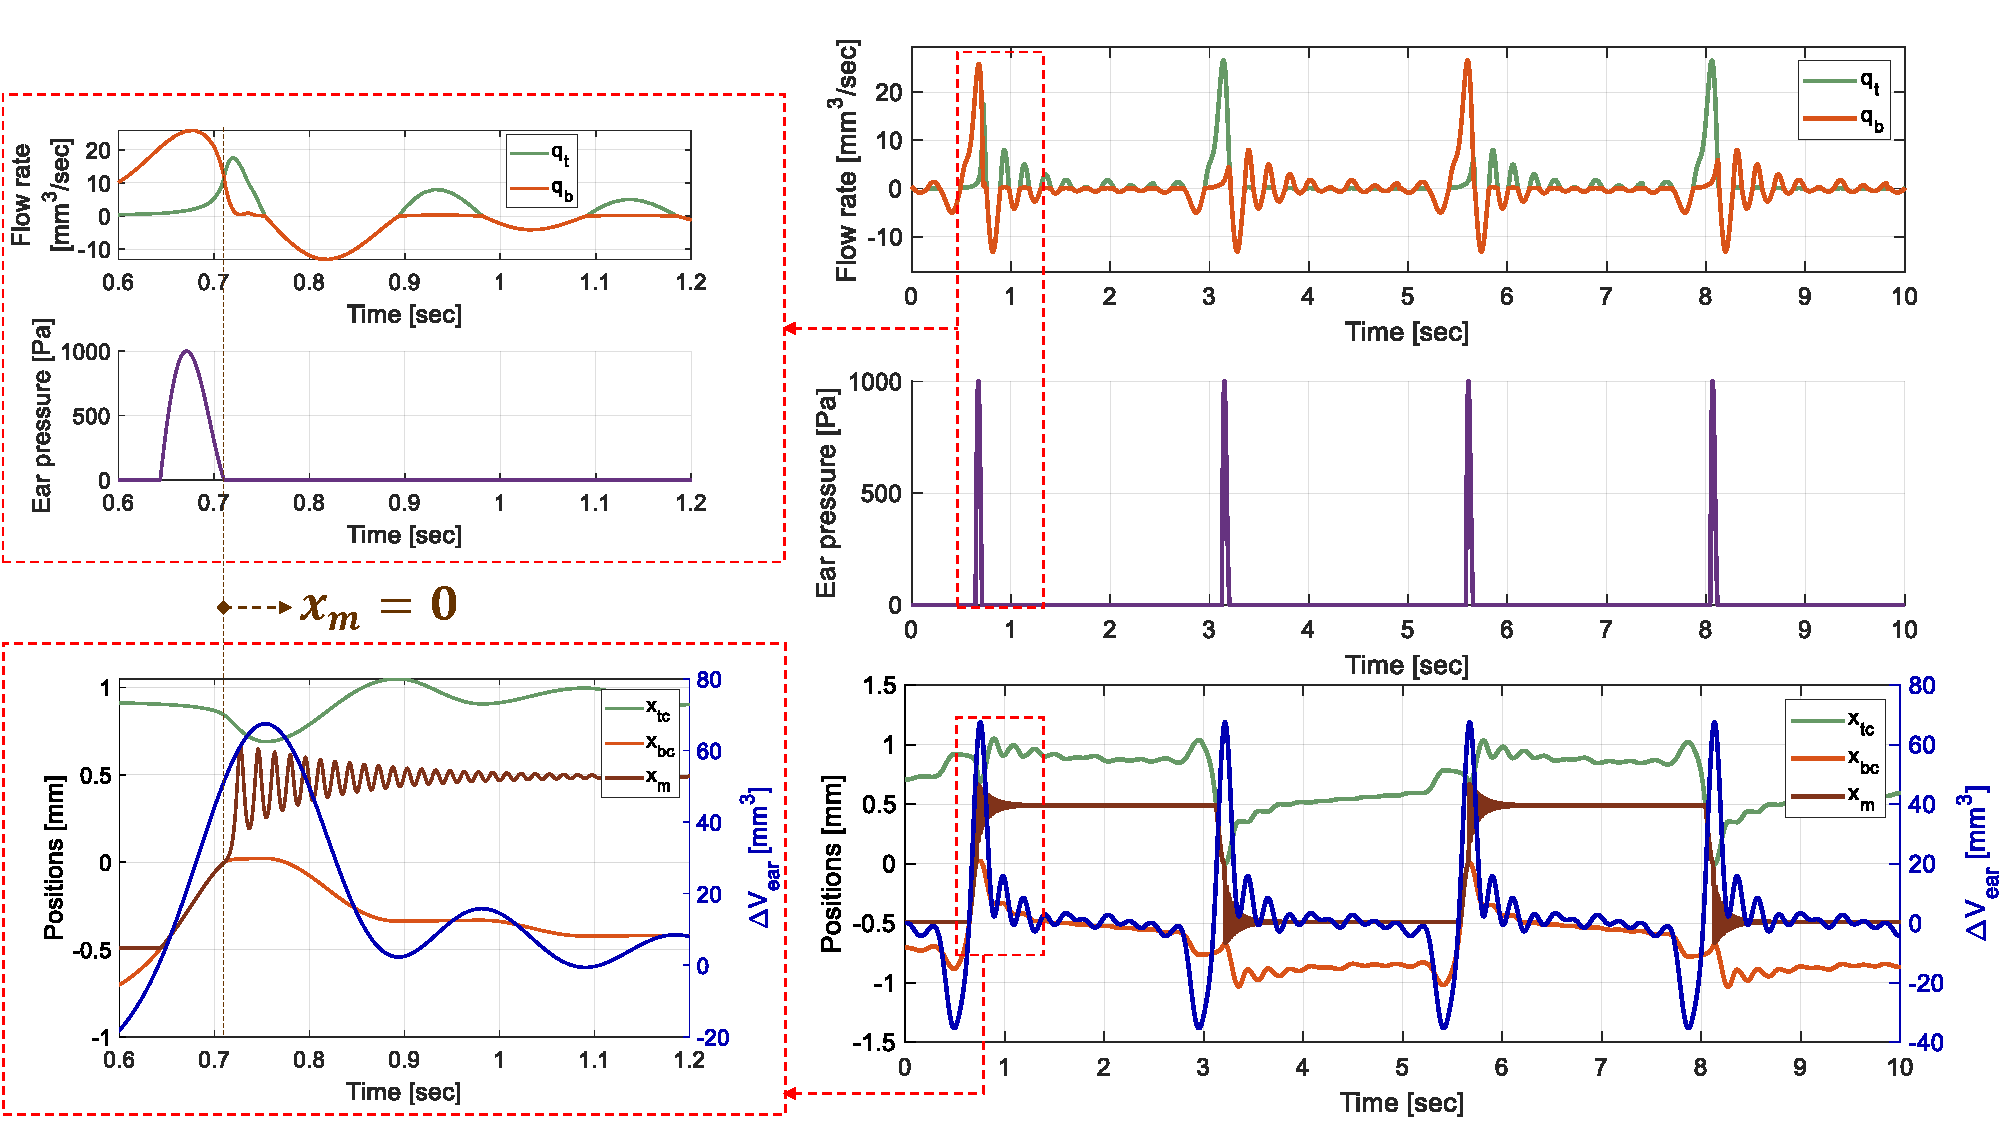
\includegraphics[trim={0cm 0cm 0cm 0.5cm},clip, width=\textwidth]{figures/positions+DeltaV_debits_pear.pdf}
	\caption{}
	\label{fig:positions+DeltaV_debits_pear}
\end{figure*}
%%%%%%%%%%%%%%%%%%%%%%%%%%%%%%%%%%%%%%%
%%%%%%%%%%%%%%%%%%%%%%%%%%%%%%%%%%%%%%
\begin{figure*}[!htbp]
	\centering
	\captionsetup{justification=centering}
	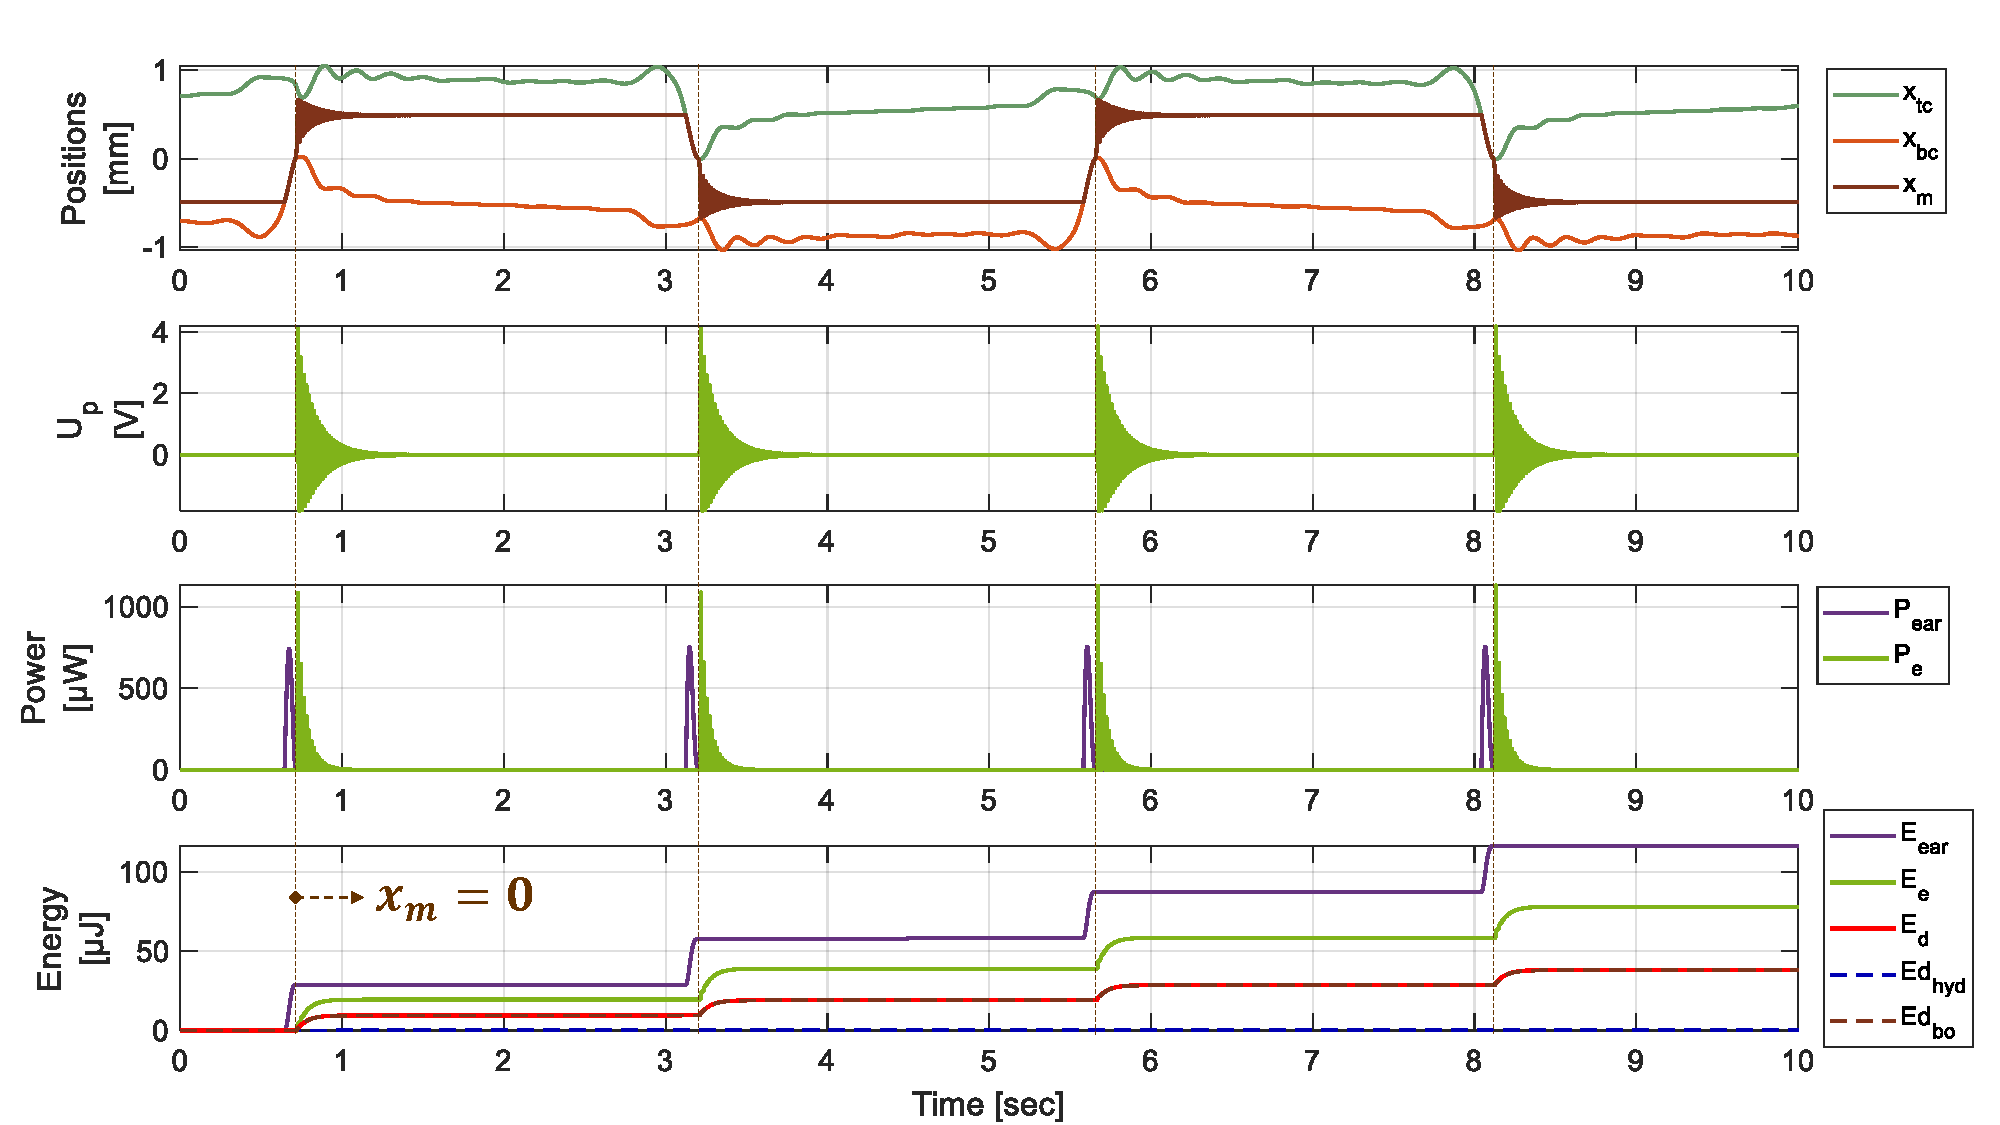
\includegraphics[trim={0cm 0cm 0cm 1cm},clip, width=\textwidth]{figures/positions_Up_puissances_energies.pdf}
	\caption{}
	\label{fig:positions_Up_puissances_energies}
\end{figure*}
%%%%%%%%%%%%%%%%%%%%%%%%%%%%%%%%%%%%%%%
%%%%%%%%%%%%%%%%%%%%%%%%%%%%%%%%%	
\begin{table}	
	\centering
	\begin{tabular}{c|c|c}
\toprule
\multicolumn{1}{c}{~~\textbf{Parameter}~~}  & \multicolumn{1}{c}{~~\textbf{Value}~~} & \multicolumn{1}{c}{~~\textbf{[Unit]}~~}  \\
\midrule
$K$					&	0.256			& [$N/\mu m$]			\\ \hline
$x_0$				&	0.49			& [$mm$] 				\\ \hline
$L$					&	16.0			& [$mm$] 				\\ \hline
$m$					&	5.88			& [$g$] 				\\ \hline
$x_{c0}$			&	0.69			& [$mm$] 				\\ \hline
$R_{ch}$			&	6.39			& [$k\Omega$] 			\\ \hline
$\alpha$			&   0.105			& [$N/V$] 				\\ \hline
$C_0$	   			&	0.25			& [$\mu F$]				\\ \hline
$Q$ 				&	50				& [-] 					\\ \hline
$\eta_g$			& 	76				& [$\%$]		\\ 
\bottomrule
	\end{tabular}
	\caption{Electromechanical parameters}
	\label{tab:parametres électromécaniques}
\end{table}
\begin{table}
	\centering
	\begin{tabular}{c|c|c}
\toprule
\multicolumn{1}{c}{~~\textbf{Parameter}~~}  & \multicolumn{1}{c}{~~\textbf{Value}~~} & \multicolumn{1}{c}{~~\textbf{[Unit]}~~}  \\
\midrule
$D_{hc}$  	   			&	4				& [$mm$]			\\ \hline
$a_h$					&	29				& [-]				\\ \hline
$p_c$					&	1				& [$kPa$]			\\ \hline
$\Delta V{ear,m}$		& 60				& [$mm^3$]			\\ \hline
$Cf_0$					&	0.21e17			&[$Pa.s^2m^{-6}$]	\\ \hline
$Cf_c$					&	5.46e17			&[$Pa.s^2m^{-6}$]	\\
\bottomrule 
	\end{tabular}
	\caption{Hydraulic parameters}
	\label{tab:parametres_hydrauliques}
\end{table}
%%%%%%%%%%%%%%%%%%%%%%%%%%%%%%%%%

The simulated model shows promising efficiency and demonstrates that a minimum value of 26 is required on the hydraulic restriction coefficient $r_{Cf}$ to ensure the adequate cycled actuation of the BR mass. Next section will present the experimental approach to validate the theoretical behavior of the electromechanical converter.

%/!\/!\/!\/!\/!\/!\/!\/!\/!\/!\/!\/!\/!\/!\/!\/!\/!\/!\/!\/!\/!\/!\/!\/!\%
\section{EXPERIMENTAL CHARACTERIZATION OF THE \mbox{ELECTROMECHANICAL} CONVERTER}
\label{sec:EXPERIMENTAL CHARACTERIZATIONS OF THE ELECTROMECHANICAL CONVERTER}
%/!\/!\/!\/!\/!\/!\/!\/!\/!\/!\/!\/!\/!\/!\/!\/!\/!\/!\/!\/!\/!\/!\/!\/!\%
    %///////////////////////////////////////////// 
	\subsection{The electromechanical converter presentation}	
	\label{The electromechanical converter presentation}
    %/////////////////////////////////////////////
The device heart is the electromechanical converter composed of the BR implementing the APG and therefore, they have been designed with respect to space requirements. We opted for a monobloc structure with blades in order to optimize the resonator quality factor by avoiding screw assemblies. Figure \ref{fig:monobloc_face} shows the face view of the monobloc bistable resonator CAD that has been fabricated by electrical discharge machining (EDM). The 8 hinges are assured by 4 buckled blades (BB) while a vertical guide blade (GB) ensures the APG mounting and avoids any of its rotations. The efficient part composed of the blades and the central mass are $1.2$mm think. The external rigid $6$mm thick frame has been designed to ensure the fixed boundary conditions and also to allow the mounting of both the measurement instruments and the HCs. The local thickenings at the midspan of the blades are intended to facilitate the fabrication and also to maximize the BB compression stiffness that maximizes the electromechanical coupling of the harvester, as we show in the following sections. The geometrical and mechanical parameters of the BR are referenced in table \ref{tab:parametres_lames}. The following sections describe the design method that led to the dimensions of the blades that depend on our needs.
%%%%%%%%%%%%%%%%%
\begin{table}[!htbp]
	\centering
    \resizebox{\linewidth}{!}{%
		\begin{tabular}{l|c|c}
			\toprule
\textbf{Parameter definition} & \textbf{Symbol}    & \textbf{Valeur [Unit]} \\
\midrule
APX4 steel Young's modulus     & $E$                       & 211 [GPa]  \\
APX4 steel elastic resistance  & $Re_{APX4}$               & 955[MPa]    \\
Dimensions of a buckled blade  & $L$ x $l$ x $e$           & 16x0.07x1.2 [mm] \\
Dimensions of the guide blade  & $L_{v}$ x $l_{v}$ x $e$   & 17.5x0.07x1.2 [mm] \\
% Mounted GB dimensions          & $L_{v2}$ x $l_{v2}$ x $e$ & 48x0.1x1.2 [mm] \\
Soft hinge stiffness		   & $K_{\varphi}$             & 0.006 [Nm/rad] \\
Stiffness of the guide blade along $\vec{y}$  & $K_{gb}$   & 190 [N/m] \\
Stiffness of 4 buckled blades along $\vec{z}$ & $K_{bb}$   & 1402 [kN/m] \\  
Stiffness of the APG along $\vec{z}$          & $K$        & 252  [kN/m]\\
			\bottomrule
		\end{tabular}}
	\caption{Definitions and values of the fabricated BR}
	\label{tab:parametres_lames}
\end{table}
%%%%%%%%%%%%%%%%%%%%% 
%%%%%%%%%%%%%%%%%%%%%%%%%%%%%%%%%%%%%%
\begin{figure}[!htbp]
\centering
\captionsetup{justification=centering}
	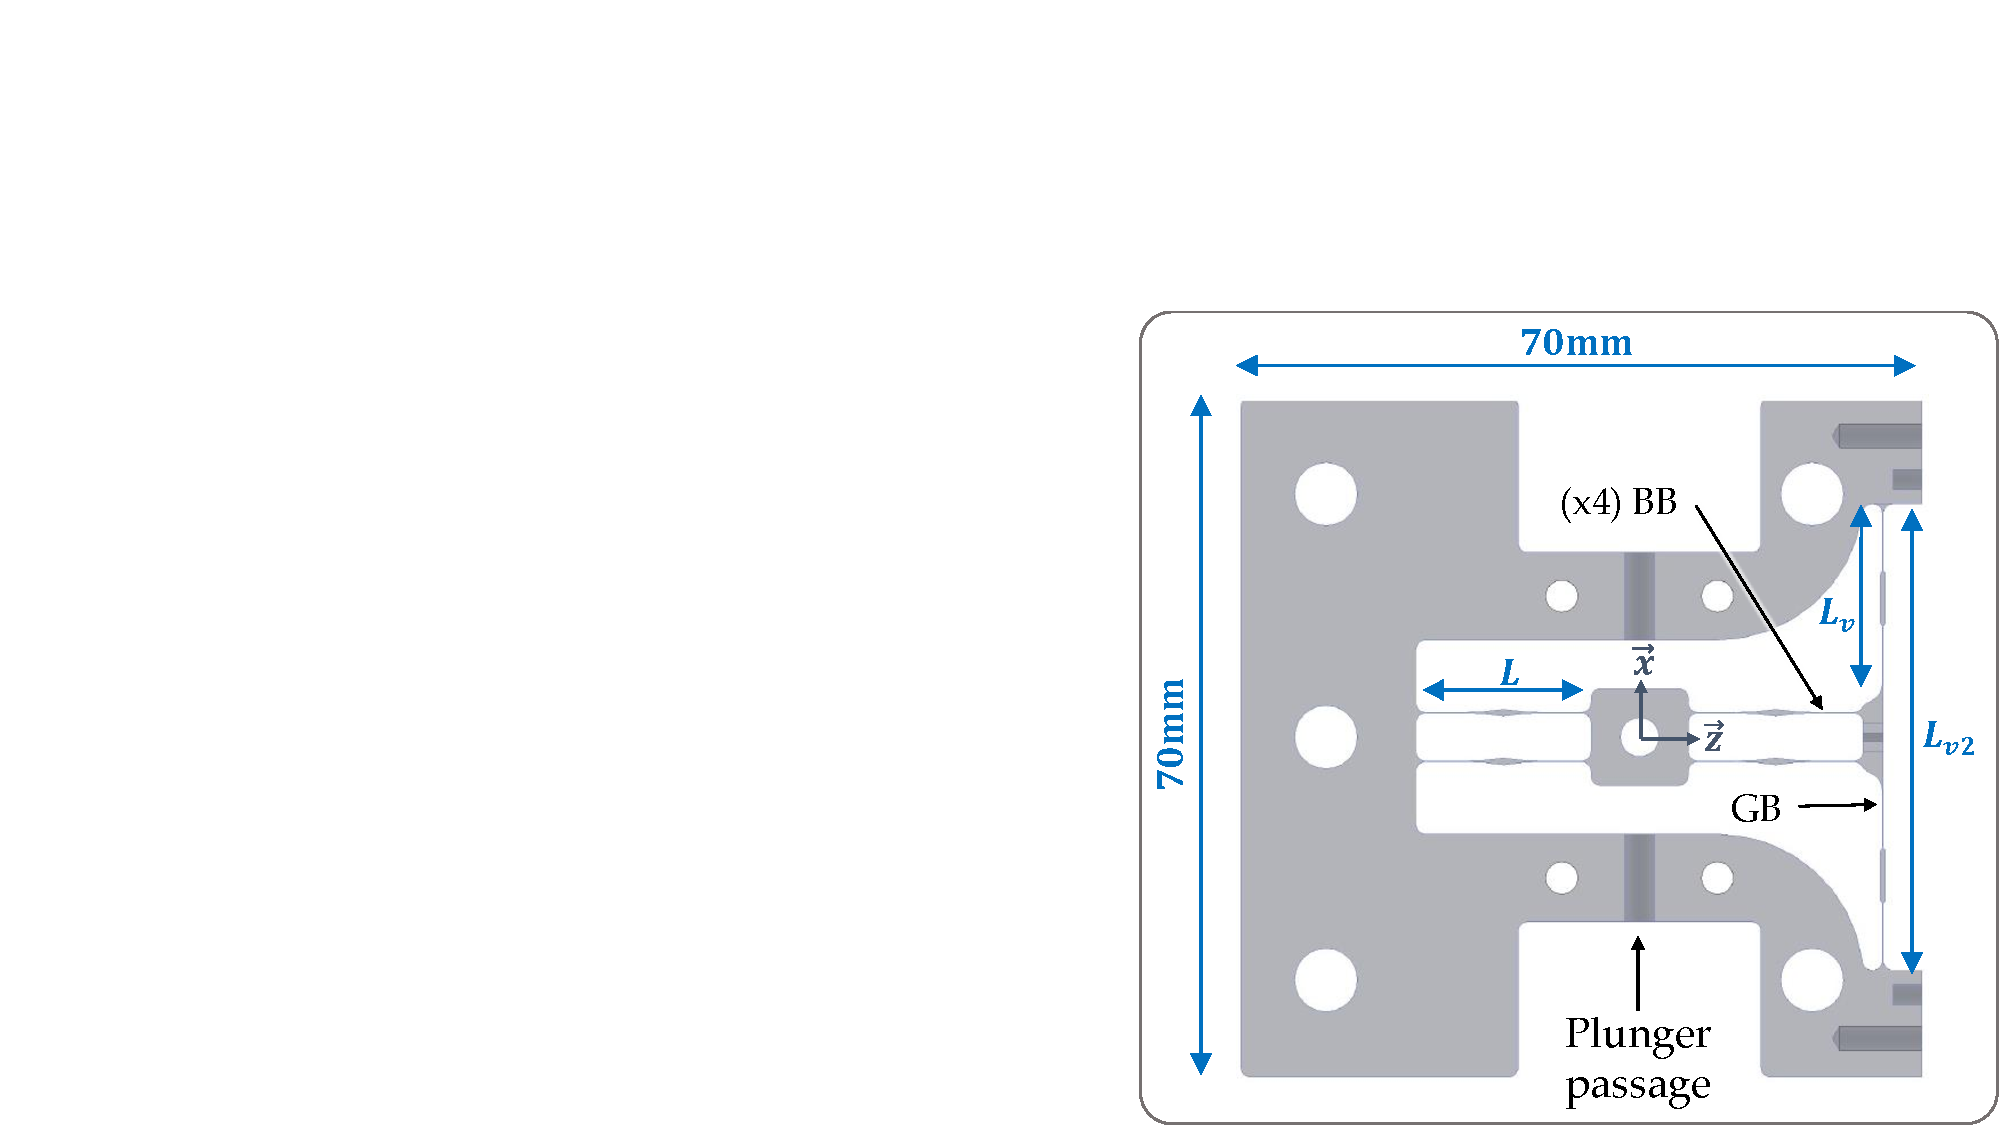
\includegraphics[trim={19.2cm 0cm 0cm 5cm},clip,width=.7\linewidth]{figures/monobloc_face.pdf}
	\caption{Face transparency view of the monobloc BR CAO}
\label{fig:monobloc_face}
\end{figure}
%%%%%%%%%%%%%%%%%%%%%%%%%%%%%%%%%%%%%%
    %///////////////////////////////////////////// 
	\subsection{BR blades design}	
	\label{subsec:BR blades design}
    %/////////////////////////////////////////////
The harvesting occurs during the free oscillation phase. The main issue is to maximize the energy conversion efficiency $\eta_{ob}$ of this stage. Richards \emph{et al.} demonstrated that for the piezoelectric transduction at the resonance frequency, it can be approximated with the equation \ref{eq:eta_ob} \cite{Richards2004}. This expression is valid for an electric extraction based on the adaptive impedance matching strategy.
\begin{equation}
	\eta_{ob} = \dfrac{k^2_{sys}\ Q}{k^2_{sys}\ Q + 2}
	\label{eq:eta_ob}
\end{equation}
Where $k^2_{sys}$ is the electromechanical coupling of the harvesting system. The latter can be expressed with the electromechanical parameters of the APG and the stiffness of the respective blades (tab. \ref{tab:parametres_lames}) as follows :
% \begin{equation}
% 	k^2_{sys} = \dfrac{ K_{bb}^2 \alpha^2 }
% 					  { \biggr(Cp(K+K_{bb} + 
% 						\dfrac{K_{bb}^2 \alpha^2}{K_{bb} + K_{gb} + K} \biggl)
% 						 (K_{bb} + K_{gb} + K)^2}
% 	\label{eq:k2_sys}
% \end{equation}

\begin{equation}
	k^2_{sys} = \dfrac{\alpha^2_{eq}}{\alpha^2_{eq} + (K+K_{gb})C_p}
	\label{eq:k2_sys}
\end{equation}
Where $\alpha_{eq}$ is the equivalent piezoelectric force factor (PFF) given by equation \ref{eq:alpha_eq}. It depends on the initial PFF of the APG alone and the and ratio between the equivalent stiffness $K_{eq}$ (eq. \ref{eq:K_eq}) of the structure on the $\vec{x}$ axis and the equivalent stiffness of the APG mounted on the GB.
\begin{equation}
	\alpha_{eq} = \alpha\ \dfrac{K_{eq}}{K + K_{gb}} 
	\label{eq:alpha_eq}
\end{equation}
\begin{equation}
	K_{eq} = \dfrac{K_{bb}(K + K_{gb})}{K_{bb} + K_{gb} + K}
	\label{eq:K_eq}
\end{equation}
Equations \ref{eq:eta_ob} - \ref{eq:K_eq} combined demonstrate that in order to maximize $\eta_{ob}$ we must make sure that $K_{bb} \gg K \gg K_{gb}$. If the condition is respected, then $K_{eq}$ can be assimilated to $K$. 

On the architecture presented on figure \ref{fig:monobloc_face} the deformation of the GB is similar to the standard case of a fixed-ended beam undergoing a single concentrated load applied at midspan. Using structural analysis formulas for this load case, we can express $K_{gb}$ as follows \cite{Leet1993} :
\begin{equation}
	K_{gb} = \dfrac{2EI_{gb}el_v^3}{L_v^3}
	\label{eq:Kgb_definition}
\end{equation}
$I_{gb}$ is the second moment of area along $\vec{y}$ axis. According the material properties and GB dimensions (tab. \ref{tab:parametres_lames}) \mbox{$K_{gb} = 190N/m$}, which is negligible before \mbox{$K=252kN/m$}.

$K_{bb}$ is for its part verified through a FEM generated with the BR CAD on ANSYS Workbench. Figure \ref{fig:fem_statique} presents the model and the initial and boundary conditions used for the study. The fixed frame is replaced by three rigid fixed points in order to minimize the number of elements and reduce the calculation time. The APG elastic force is modeled by the load $F_{st}$ applied at the right end of the structure and the transducer is replaced by a rigid mobile part in order to isolate the stiffness of the BBs.
%%%%%%%%%%%%%%%%%%%%%%%%%%%%%%%%%%%%%%
\begin{figure}[!htbp]
\centering
\captionsetup{justification=centering}
	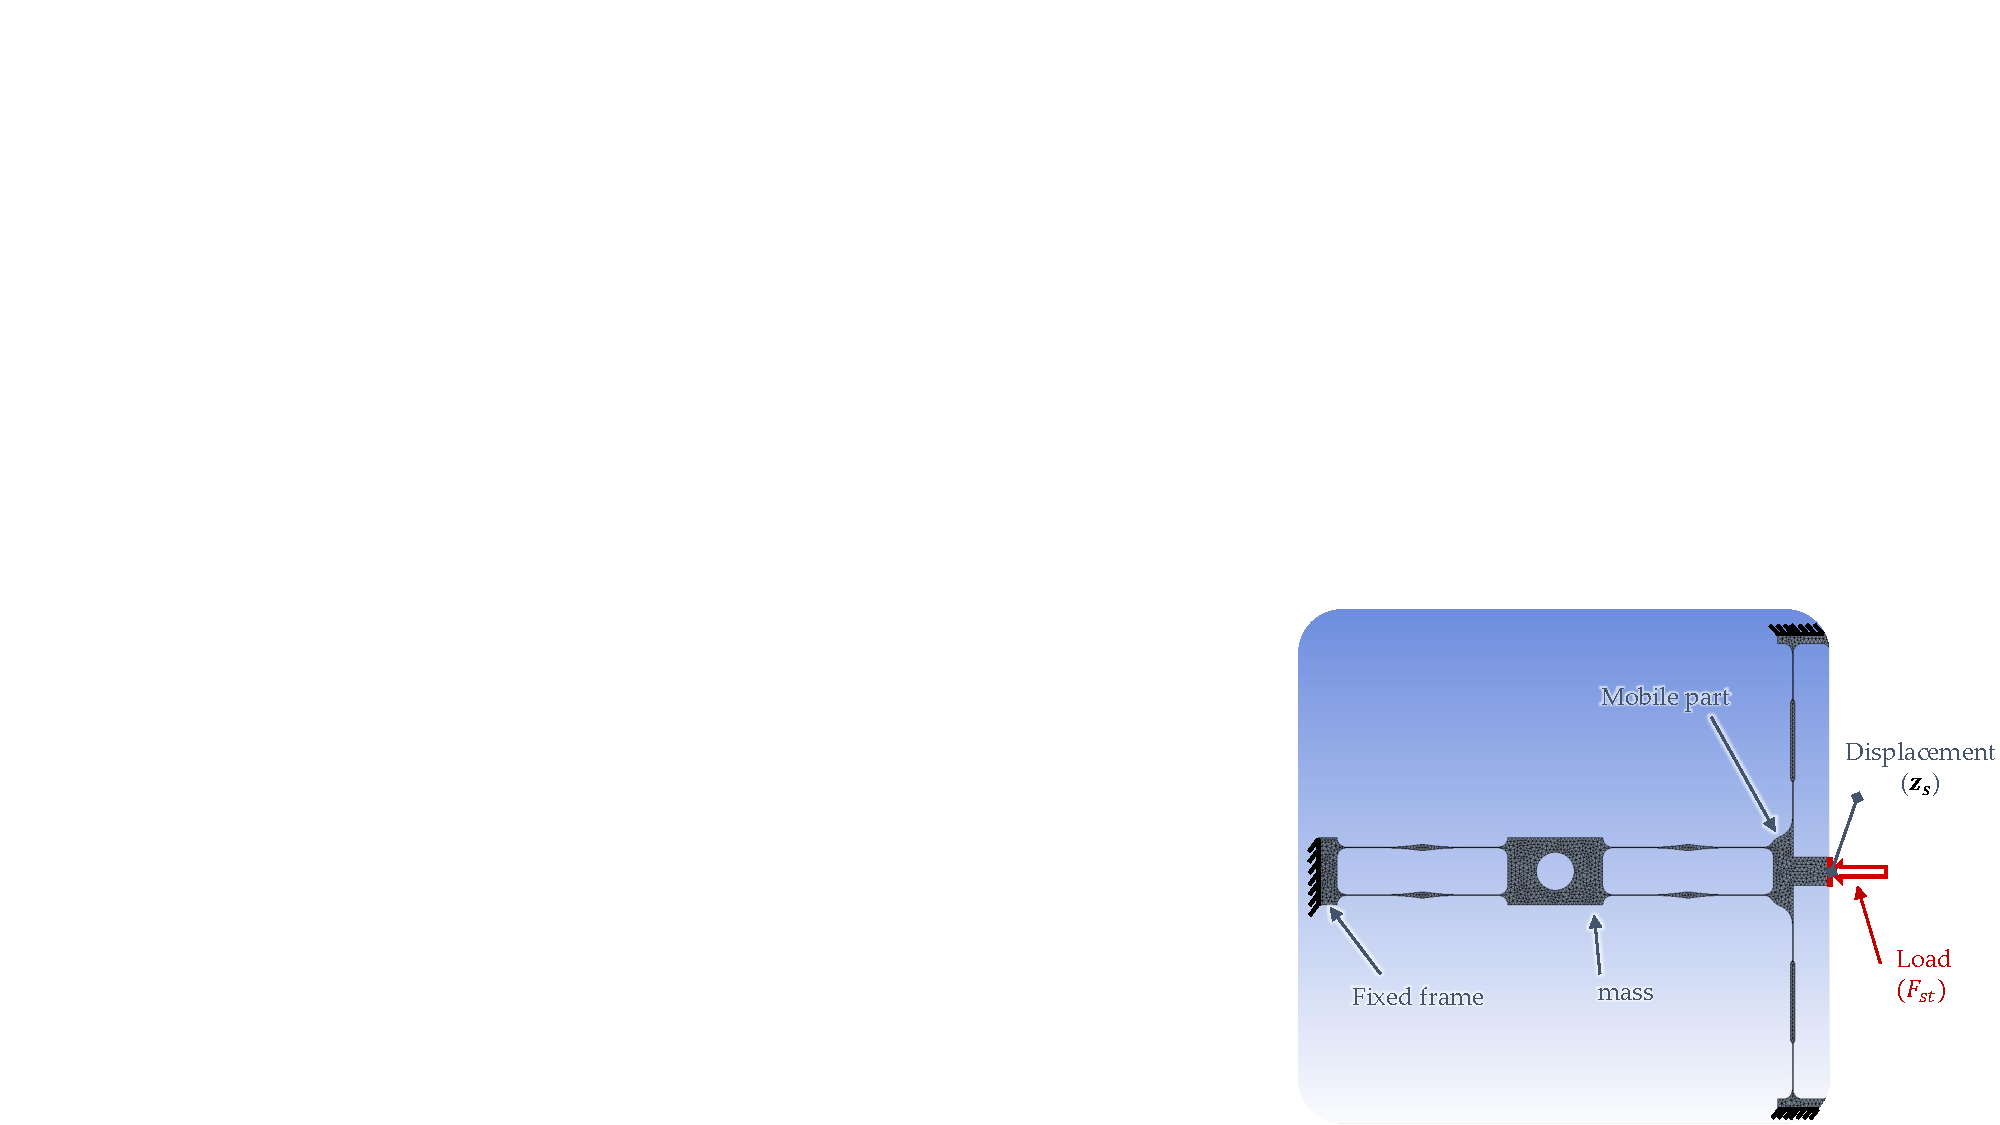
\includegraphics[trim={21.9cm 0cm 0cm 10.2cm},clip,width=.8\linewidth]{figures/fem_statique.pdf}
	\caption{BR finit element model with initial and boundary conditions for a static study}
\label{fig:fem_statique}
\end{figure}
%%%%%%%%%%%%%%%%%%%%%%%%%%%%%%%%%%%%%%
By imposing incrementally increasing $F_{st}$ and measuring the displacement $z_{st}$ of the moving structure in small displacement condition, we can determine $K_{bb}$ (tab. \ref{tab:parametres_lames}) with equation \ref{eq:Kbb_definition}. The stiffness of the BBs and the GB lead to a theoretical efficiency of 75\%, which is consistent with the previous simulated results (tab. \ref{tab:parametres électromécaniques}).
\begin{equation}
	K_{bb} = \dfrac{F_{st}}{z_{st}}
	\label{eq:Kbb_definition}
\end{equation}
%%%%%%%%%%%%%%%%%%%%%%%%%%%%%%%%%%%%%%

In order to preserve an adequate mechanical transmission from the mass to the APG, we must ensure that no secondary buckling mode does appear on the BBs during the BR operation. Based on the precedent FEM static model (fig. \ref{fig:fem_statique}), a buckling study has been performed for the purpose. When the mass crosses the unstable \mbox{$x_m=0$} position, the compression stress on the blades is in fact at its maximum. With the same boundary conditions as in figure \ref{fig:fem_statique}, the buckling study imposes the force $F_{st} = F_{z,0}$ modeling the APG elastic counter reaction on $\vec{z}$ axis at $x_m = 0$. $F_{z,0}$ can be expressed by equation \ref{eq:Fz0_flambement} relying on figure \ref{fig:schema_cinematique1} :
\begin{equation}
	F_{z,0} = 2K \biggl( \sqrt{x_0^2+L^2}-L \biggr)
	\label{eq:Fz0_flambement}
\end{equation}

The fundamental buckling mode of the BBs leads to the wanted structural buckling generating the bistable equilibrium positions $\pm x_0$ for the mass. The buckling study reveals that $F_{z,0}=0.61$N when the useful buckling mode appears (fig. \ref{fig:buckling_fundamental}). However, the first secondary undesirable mode illustrated on figure \ref{fig:buckling_secondary} appears for $F_{z,0}=6.4$N. 

%%%%%%%%%%%%%%%%%%%%%%%%%%%%%%%%%%%%	
\begin{figure}[!htb]
	\begin{center}
		\begin{subfigure}[t]{0.48\linewidth}
			\captionsetup{justification=centering}
			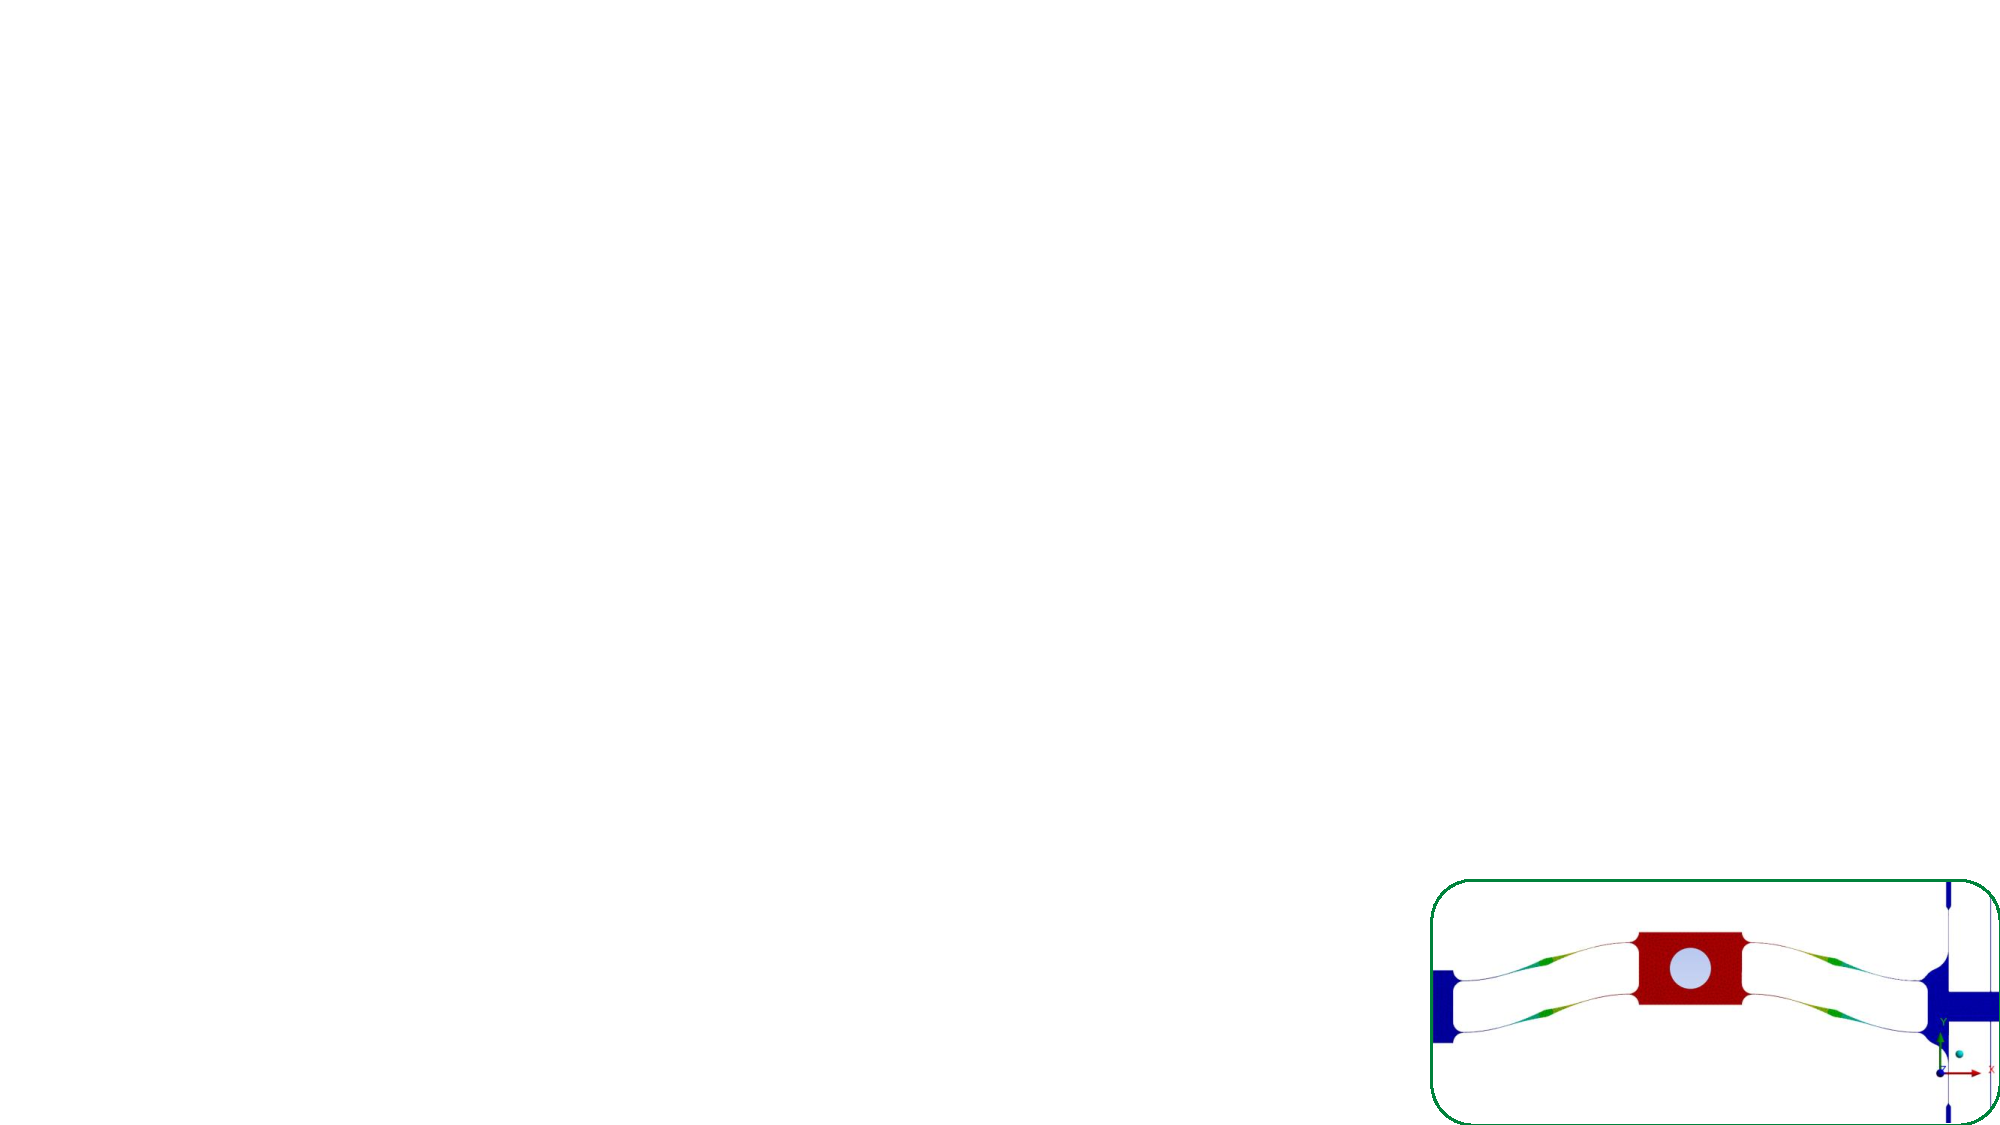
\includegraphics[trim={24.1cm 0cm 0cm 14.8cm},clip,width=\linewidth]{figures/buckling_fundamental.pdf}
			\caption{Fundamental = useful}
			\label{fig:buckling_fundamental}
		\end{subfigure}
		\hfillx
		\begin{subfigure}[t]{0.48\linewidth}
			\captionsetup{justification=centering}
			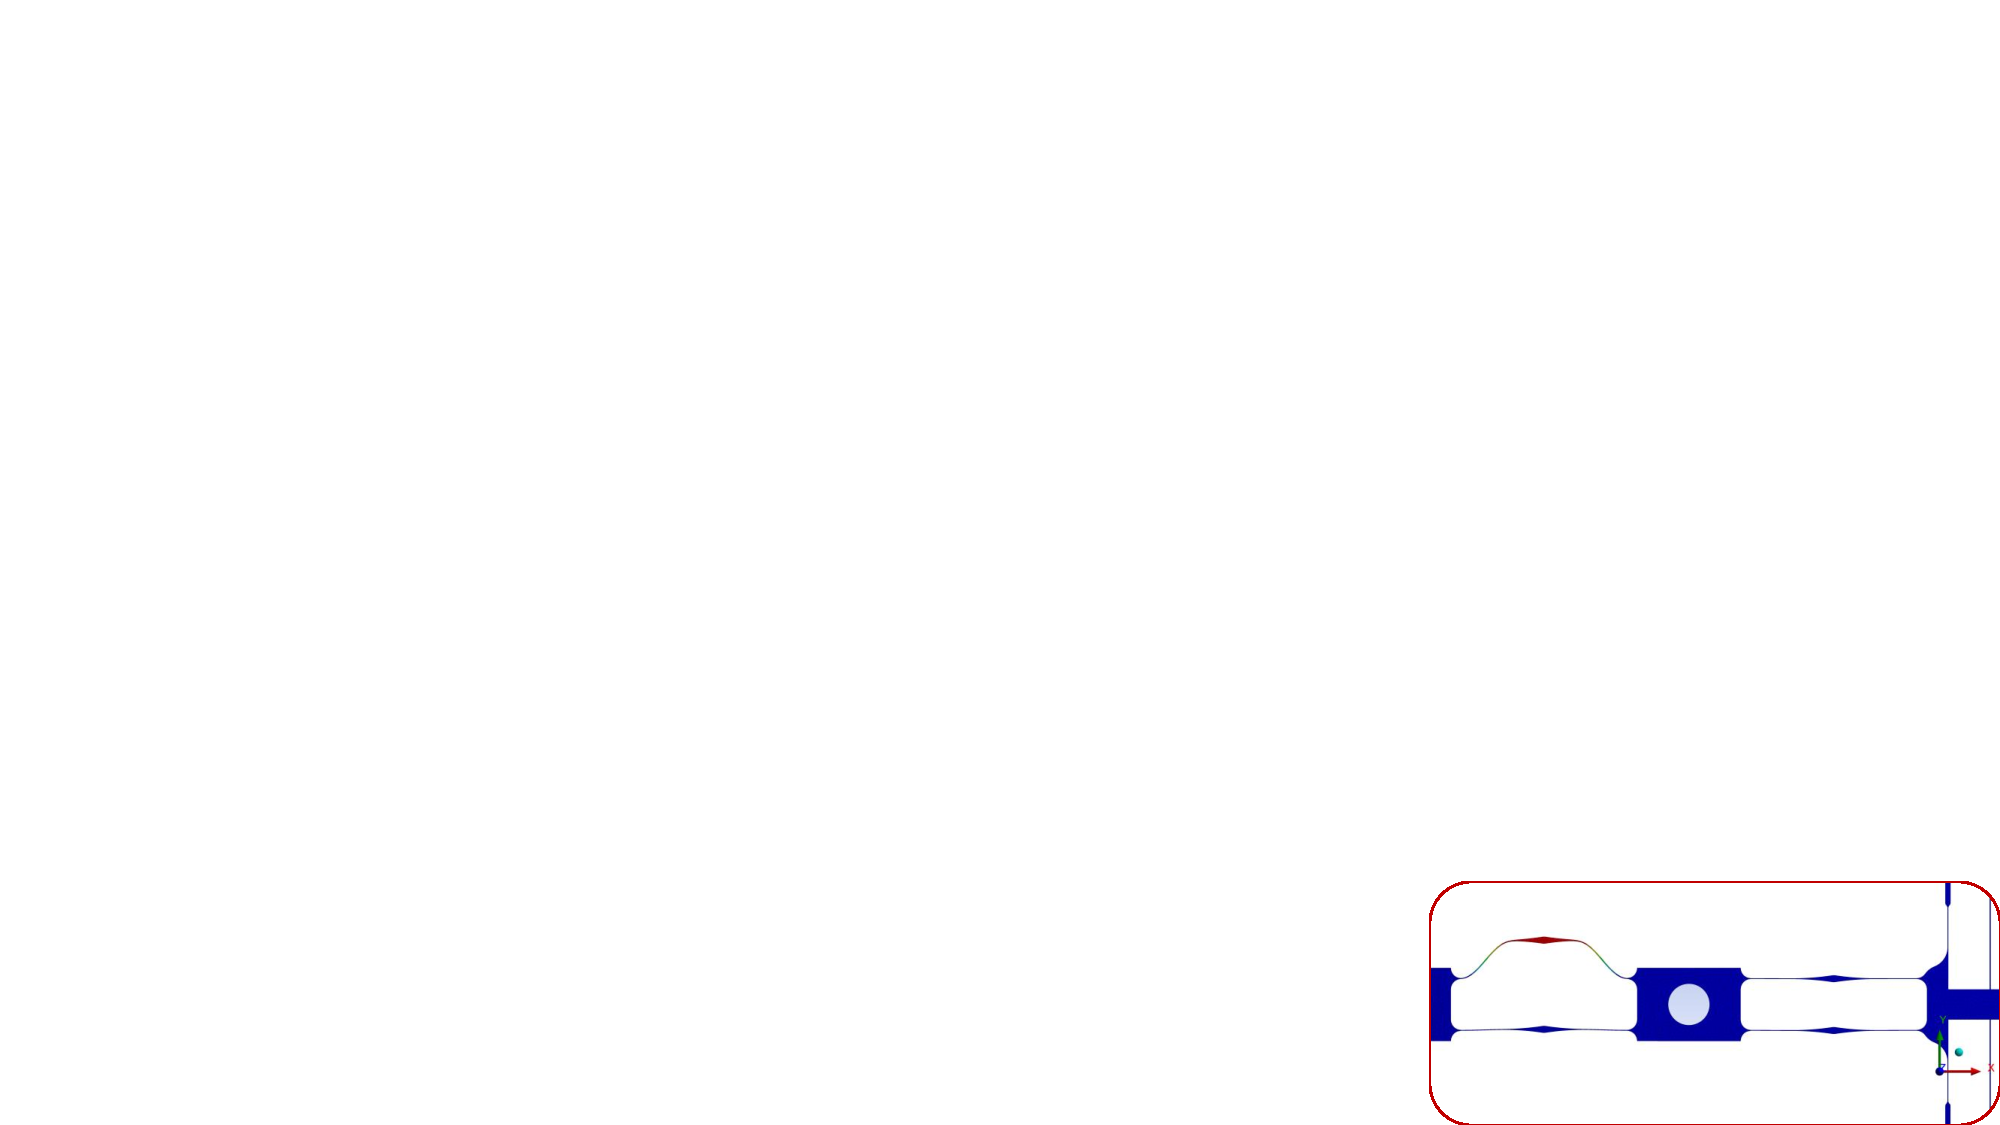
\includegraphics[trim={24.1cm 0cm 0cm 14.8cm},clip,width=\linewidth]{figures/buckling_secondary.pdf}
			\caption{Secondary = undesirable}
			\label{fig:buckling_secondary}
		\end{subfigure}
		\caption{Deformed shape of the first appearing buckling modes}
		\label{fig:Buckling_deformed_shapes}
	\end{center}
\end{figure}
%%%%%%%%%%%%%%%%%%%%%%%%%%%%%%%%%%%% 
The secondary buckling modes absorb mechanical energy that is not transmitted to the APG and therefore can not be converted in electricity. Therefore, it is preferable to avoid them by establishing a buckling height domain for the fabricated BR, as presented on figure \ref{fig:buckling_limit}. The preliminary simulated case presented in the previous section is well located in the preferable domain where there is no undesirable buckling modes. Moreover, the force absorbed by the APG is well under the maximal limit of 18N from which the device could be damaged.
%%%%%%%%%%%%%%%%%%%%%%%%%%%%%%%%%%%%%%
\begin{figure}[!htbp]
	\centering
	\captionsetup{justification=centering}
	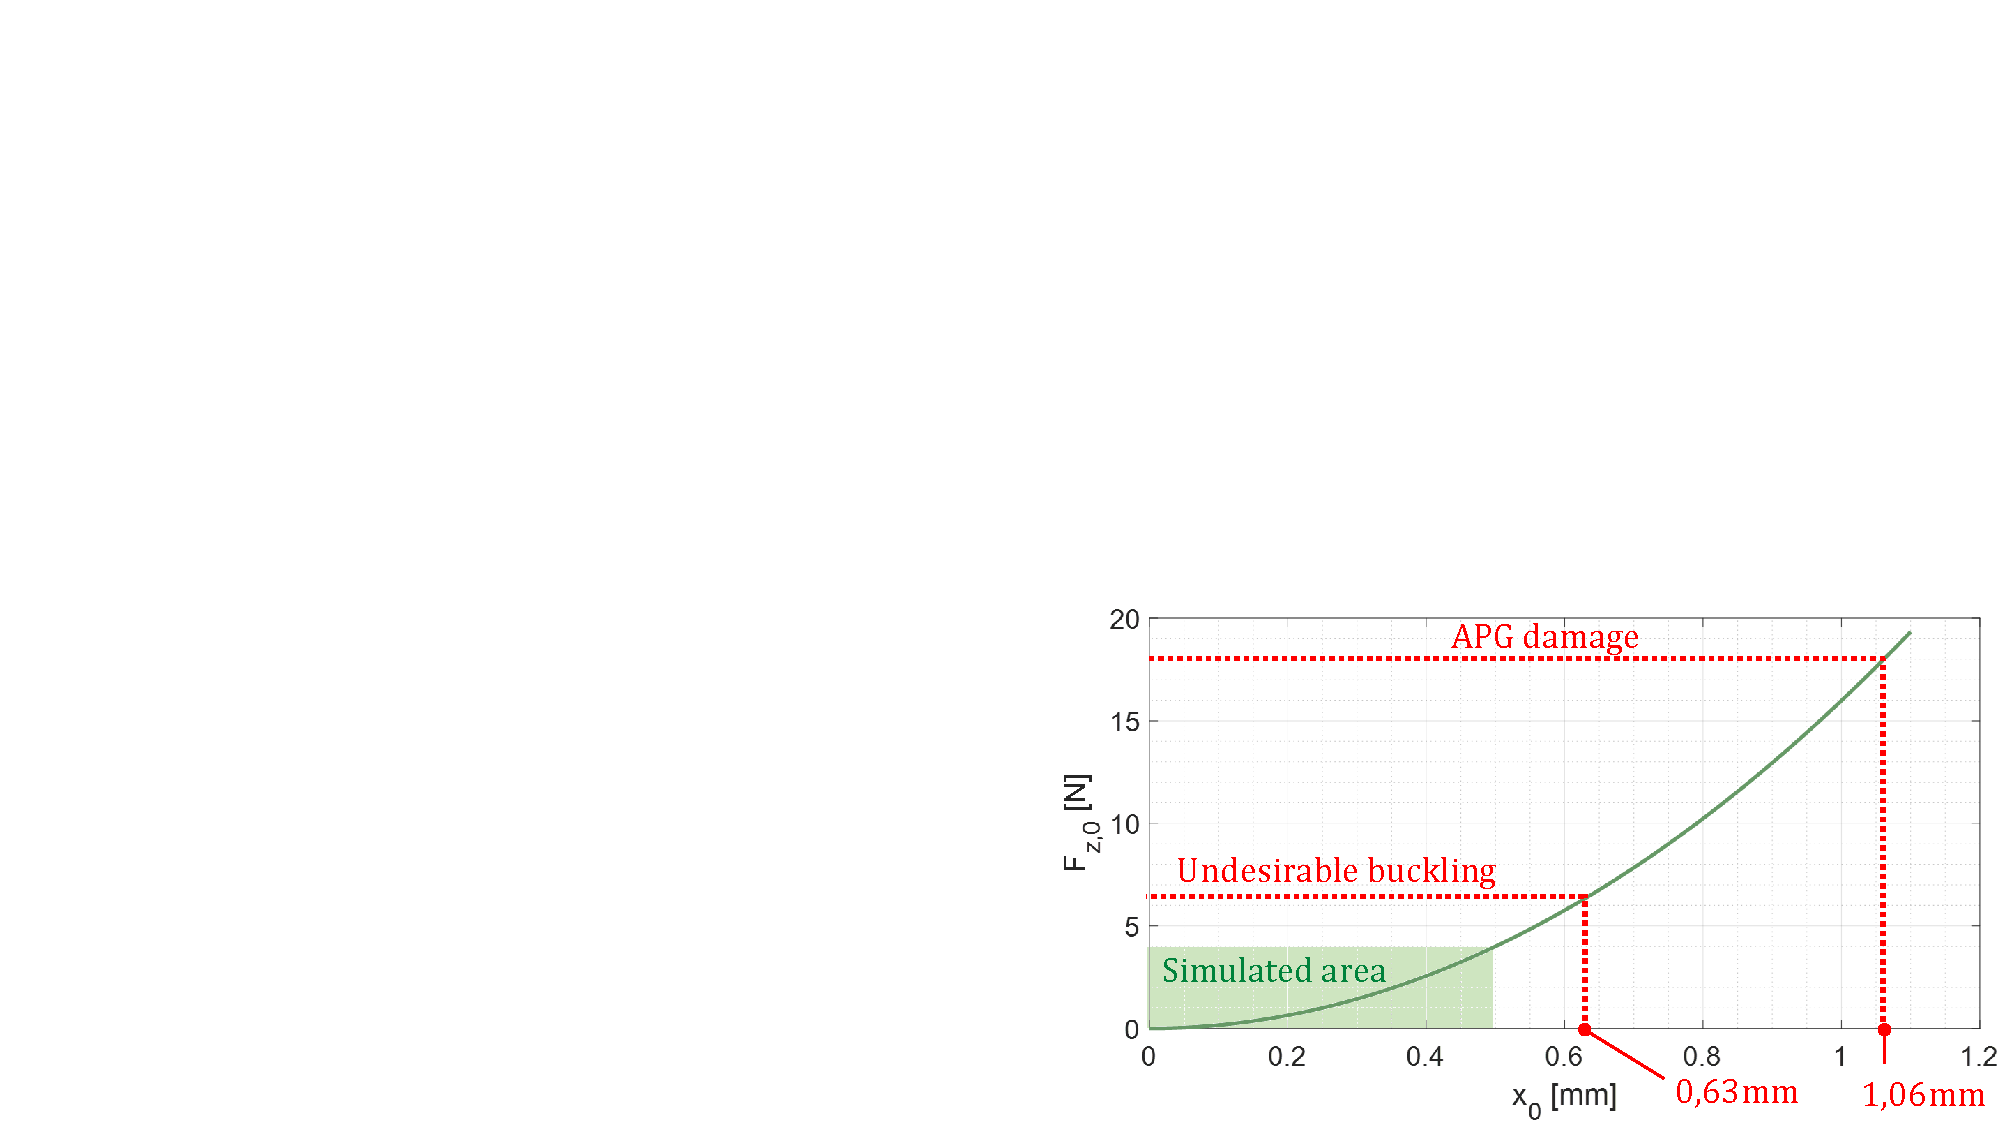
\includegraphics[trim={17.9cm 0cm 0cm 10cm},clip,width=0.9\linewidth]{figures/buckling_limit.pdf}
	\caption{APG elastic counter reaction on $\vec{z}$ axis at $x_m=0$, depending on the initial structural buckling height $x_0$}
	\label{fig:buckling_limit}
\end{figure}
%%%%%%%%%%%%%%%%%%%%%%%%%%%%%%%%%%%%%%
% Ltex language=en

    %///////////////////////////////////////////// 
	\subsection{Experimental characterizations}	
	\label{subsec:Experimental characterizations}
    %/////////////////////////////////////////////
The BR has been fabricated and mounted and the APG has been implemented on it. The experimental test bench for the electromechanical characterizations of the resultant converter is presented on figure \ref{fig:BDT_OB+GPA}. An additional blade is mounted with the APG in order to prevent its rotation around any axis. A micrometric screw helps to set the initial structural buckling level $x_0$ ($\pm 10$µm). The bearing decouples the rotation of the screw with the rotation of the blade structure in order to prevent unwanted torsional stress. Two symmetrically mounted masses are added on the initial central mass with a 45\degree{} machined plane. The latter receives and reflects the displacement sensor emitted laser along the $\vec{z}$ axis and allows to get the $x_m$ position of the mas along $\vec{x}$ axis ($\pm 10$µm). The APG power is dissipated in the $R_{ch}$ resistor and the $U_p$ tension ($\pm 1$mV), along with $x_m$, are monitored through a data acquisition card NI-USB 6212 and a LabVIEW interface. Finally, the two HC plungers actuate the mass from one stable equilibrium position to the other.
%%%%%%%%%%%%%%%%%%%%%%%%%%%%%%%%%%%%%%
\begin{figure}[!htbp]
	\centering
	\captionsetup{justification=centering}
	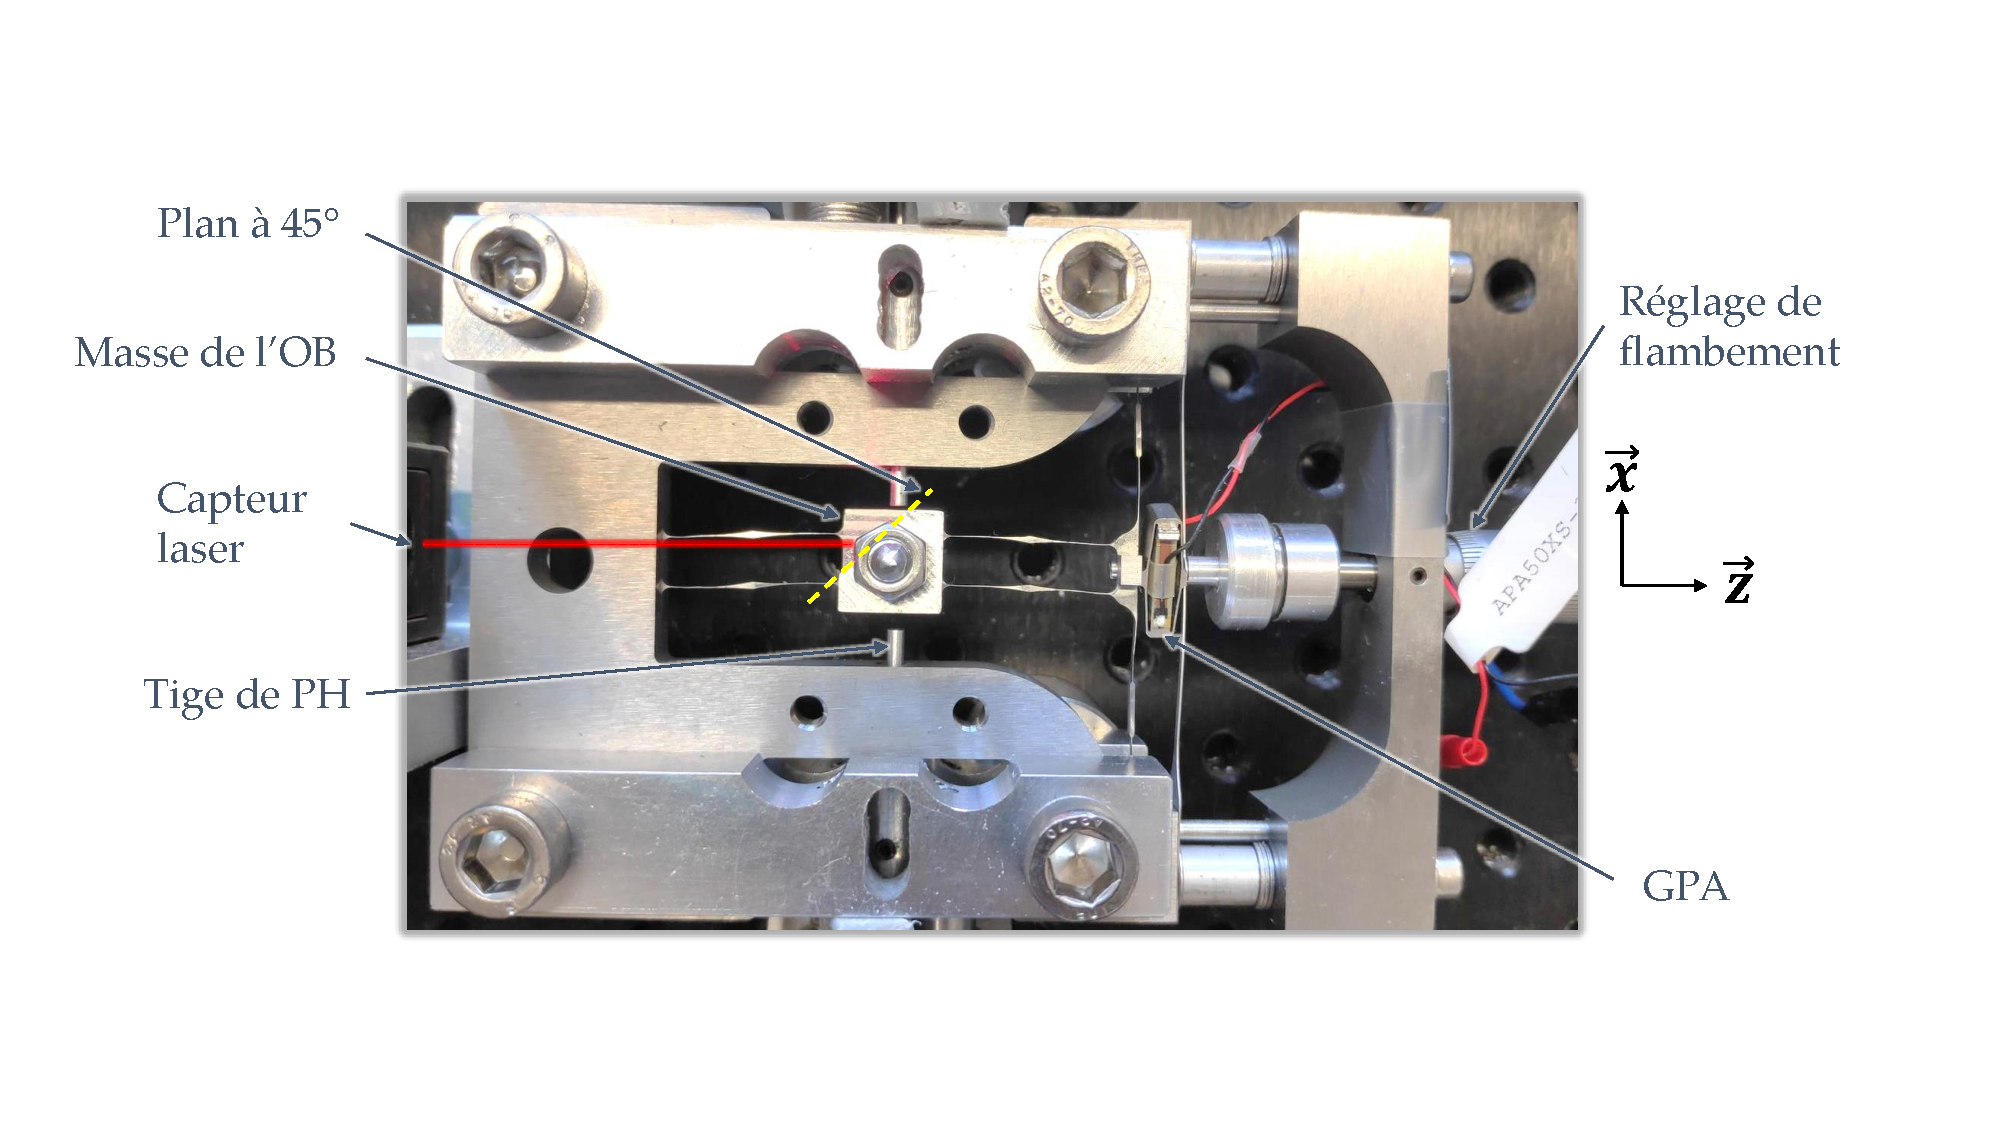
\includegraphics[trim={2cm 0cm 0cm 5.5cm},clip,width=\linewidth]{figures/BDT_OB+GPA.pdf}
	\caption{Test bench of the electromechanical converter}
	\label{fig:BDT_OB+GPA}
\end{figure}
%%%%%%%%%%%%%%%%%%%%%%%%%%%%%%%%%%%%%%%
The HV mechanical influence is not considered in order to isolate the electromechanical converter dynamic behavior. The test protocol consisted on recreating the operation conditions as close as possible to real-life operation. The mass is guided from a stable equilibrium position until it reaches \mbox{$x_m=0$}, and then it goes oscillate around the opposite stable equilibrium position. The experimental data was then used to identify and recalibrate the following electromechanical parameters of the harvester through iterative simulations of the global \mbox{model :} $Q$, $f_0$, $K$ and $k_{sys}^2$ (tab. \ref{tab:parametres_lacher_free}). The correlations were made with iterative simulations of the global model by minimizing the error between the simulated and the experimental parameters. The experimental oscillation frequency $f_0$ and energy conversion efficiency $\eta_{br}$ of the converter have also been extracted from the recalibrated model. The simulation with the recalibrated parameters and the experimental data are superposed on figure \ref{fig:BDT_OB+GPA}. The experimental data have been fitted on the oscillation phase of the simulated global model as the test bench does not reproduce the hydraulic circuit behavior yet.
%%%%%%%%%%%%%%%%%
\begin{table}[!htbp]
\centering
\captionsetup{justification=centering}
	\begin{tabular}{ c | c | c }
	\toprule
	& \textbf{Simulation with}  	   & \textbf{Simulation with}       \\
	& \textbf{theoretical}  		   & \textbf{recalibrated }		 	\\
	\multirow{-3}{*}{\textbf{Symbol}}
	& \textbf{parameters}			   & \textbf{parameters} 			\\
	\midrule
	$Q$                       & 50.0                  & 30.0 		  	\\  
	$f_0$                     & 47.0 Hz               & 27.9 Hz  		\\
	$x_0$                     & 0.49 mm               & 0.50 mm    		\\
	$K$                       & 2.56e5 N/m            & 0.85e5 N/m 		\\
	${k^2_{sys}}$             & 16 \%                 & 1.25 \% 		\\
	$\eta_{br}$               & 75 \%                 & 12.9 \%   		\\
	\bottomrule
	\end{tabular}
	\caption{Theoretical and experimentally recalibrated values of the electromechanical converter.}
	\label{tab:parametres_lacher_free}
\end{table} 
%%%%%%%%%%%%%%%%%%%%%  
%%%%%%%%%%%%%%%%%%%%%%%%%%%%%%%%%%%%%%
\begin{figure}[!htbp]
	\centering
	\captionsetup{justification=centering}
	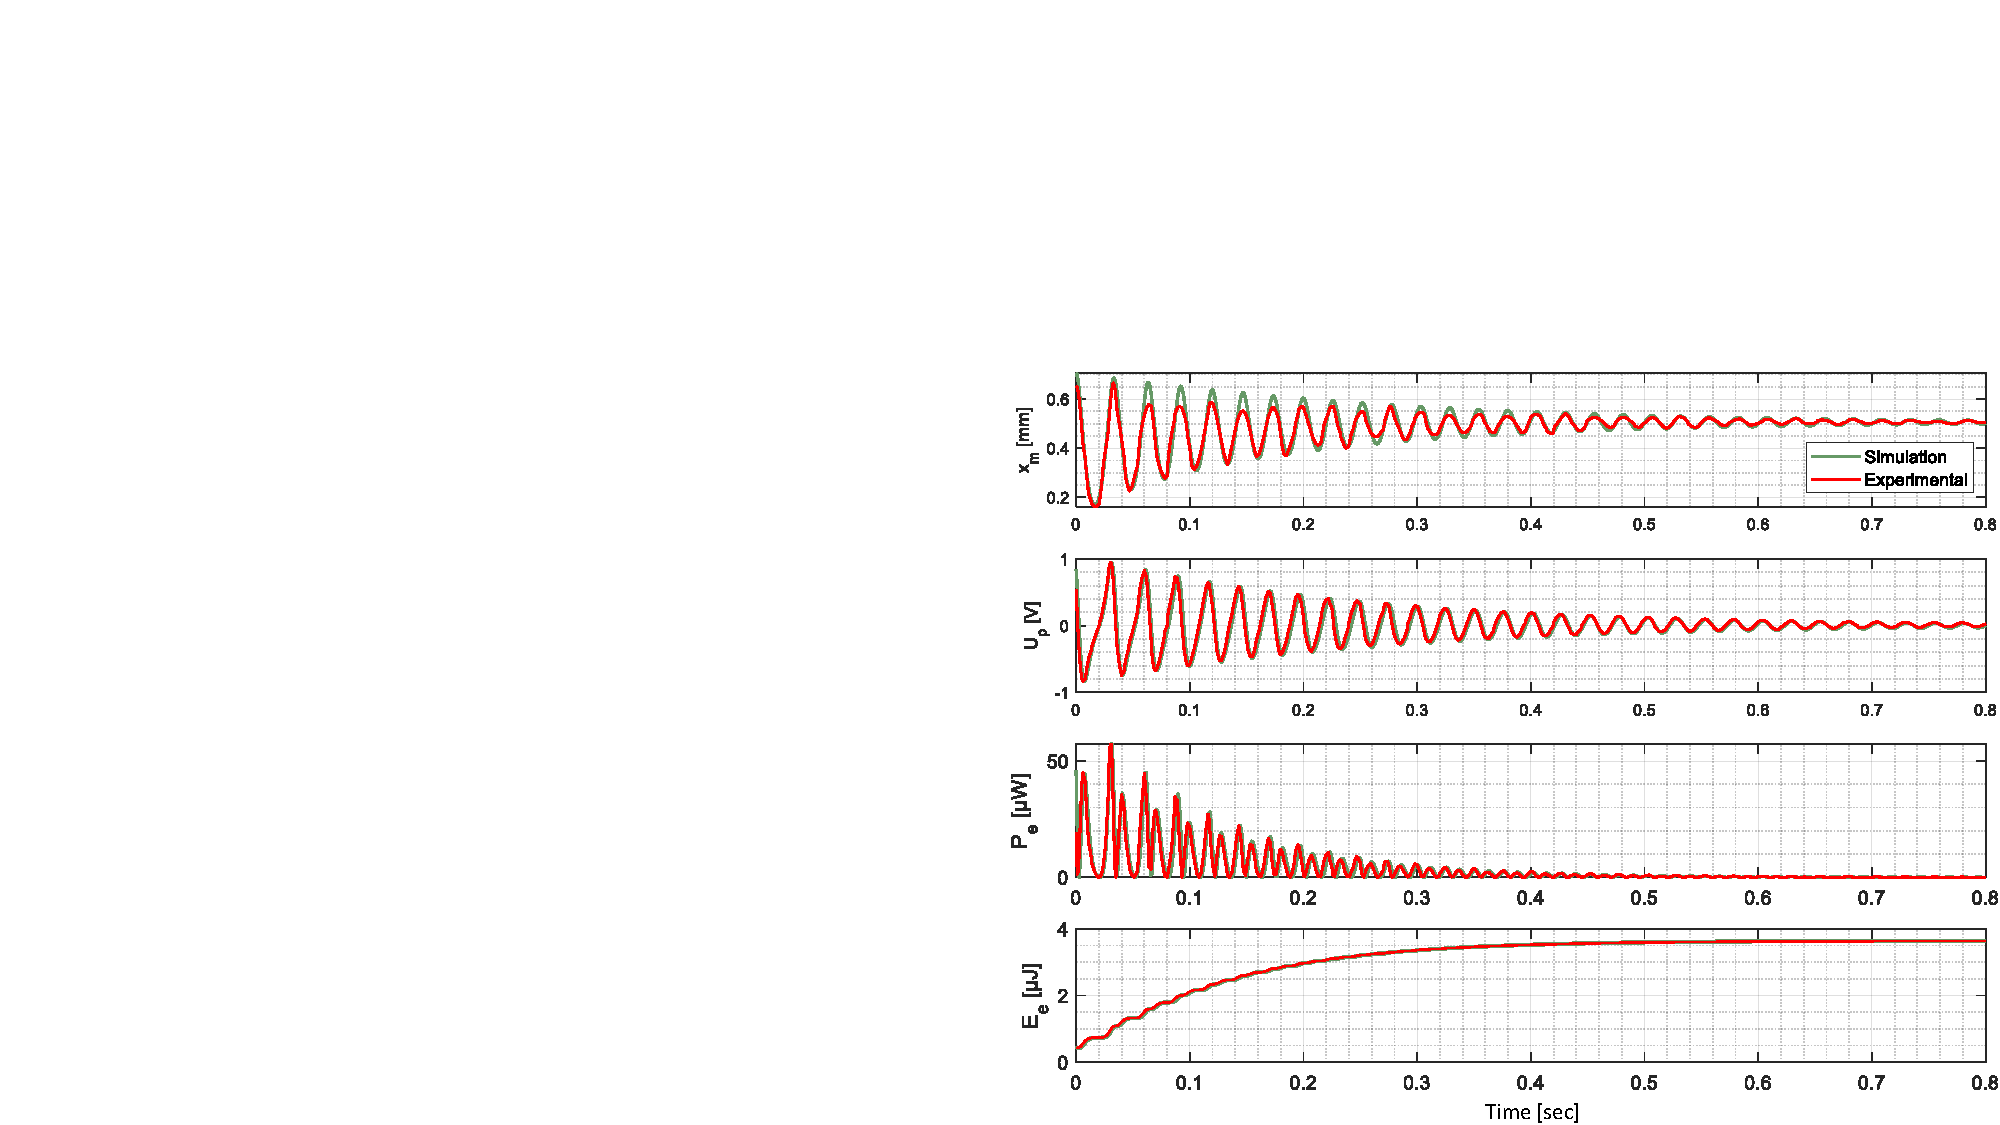
\includegraphics[trim={17cm 0cm 0cm 6cm},clip,width=\linewidth]{figures/correlation_simu-exp_OB+GPA.pdf}
	\caption{Experimental measurements and global system simulation with the identified parameters of table \ref{tab:parametres_lacher_free}.}
	\label{fig:BDT_OB+GPA}
\end{figure}
%%%%%%%%%%%%%%%%%%%%%%%%%%%%%%%%%%%%%%%

    %///////////////////////////////////////////// 
	\subsection{Analyze and summary}	
	\label{subsec:Analyze and summary}
    %/////////////////////////////////////////////

According to figure \ref{fig:BDT_OB+GPA}, the experimental dynamics of the converter is predictable by the equations established after identification of the system parameters listed in table \ref{tab:parametres_lacher_free}. However, the performances of the experimental prototype proved to be below the values theoretically predicted (tab. \ref{tab:parametres électromécaniques}) even if the efficiency drop is consistent with the quality factor and the electromechanical coupling coefficient drop (eq. \ref{eq:eta_ob}). We identified two main factors that could have led to such results. 

First, the quality factor decrease could be related to the general non-permanent assembly that uses non-perfect embeddings with fixation screws and a mobile micrometric screw. 
Then, small undulations have been observed on the BBs after fabrication, and they could also have gotten worse during the manipulation.


%/!\/!\/!\/!\/!\/!\/!\/!\/!\/!\/!\/!\/!\/!\/!\/!\/!\/!\/!\/!\/!\/!\/!\/!\%
\section{EXPERIMENTAL APPROACH FOR THE HV \mbox{DESIGN}}
\label{sec:EXPERIMENTAL APPROACH FOR THE HV DESIGN}
%/!\/!\/!\/!\/!\/!\/!\/!\/!\/!\/!\/!\/!\/!\/!\/!\/!\/!\/!\/!\/!\/!\/!\/!\%

    %///////////////////////////////////////////// 
	\subsection{The HV hydraulic behavior}	
	\label{The hydraulic valves}
    %/////////////////////////////////////////////

	%/////////////////////////////////////////////
	\subsubsection{Test bench presentation}
	 %/////////////////////////////////////////////

	%/////////////////////////////////////////////
	\subsubsection{Results and discussion}
    %/////////////////////////////////////////////


\begin{figure*}[!htb]
\begin{center}
	\captionsetup{justification=centering} 
	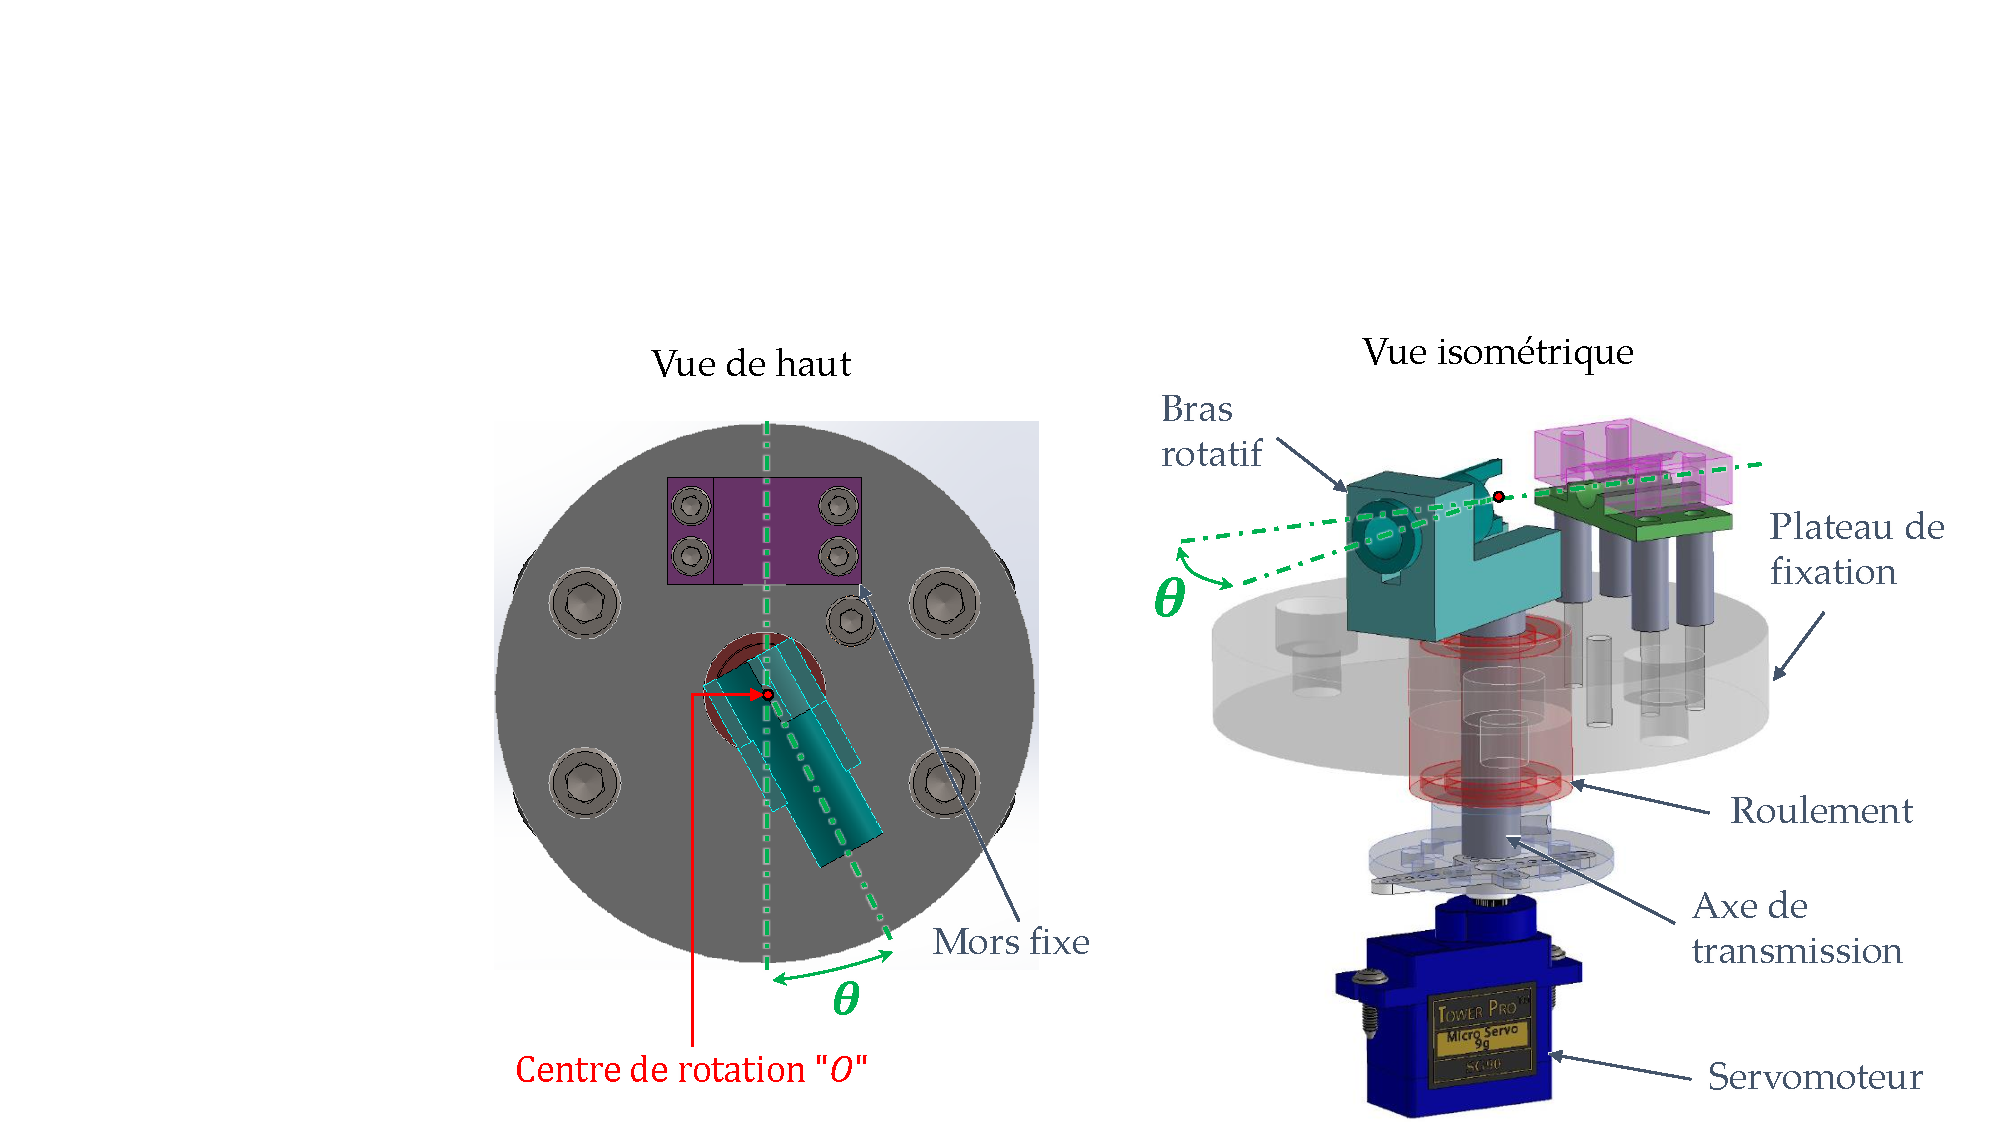
\includegraphics[trim={8cm 0cm 0cm 5cm},clip,width=0.8\textwidth]{figures/BDT_hydraulique_VH.pdf}
	\caption{Banc d'essai pour la caractérisations hydrauliques de VH}
	\label{fig:BDT_hydraulique_VH}
\end{center}	
\end{figure*}    
%%%%%%%%%%%%%%%%%%%%%%%%%%%%%%%%%%%% 
%%%%%%%%%%%%%%%%%%%%%%%%%%%%%%%%%%%%	
\begin{figure*}[!htb]
\begin{center}
	\captionsetup{justification=centering} 
	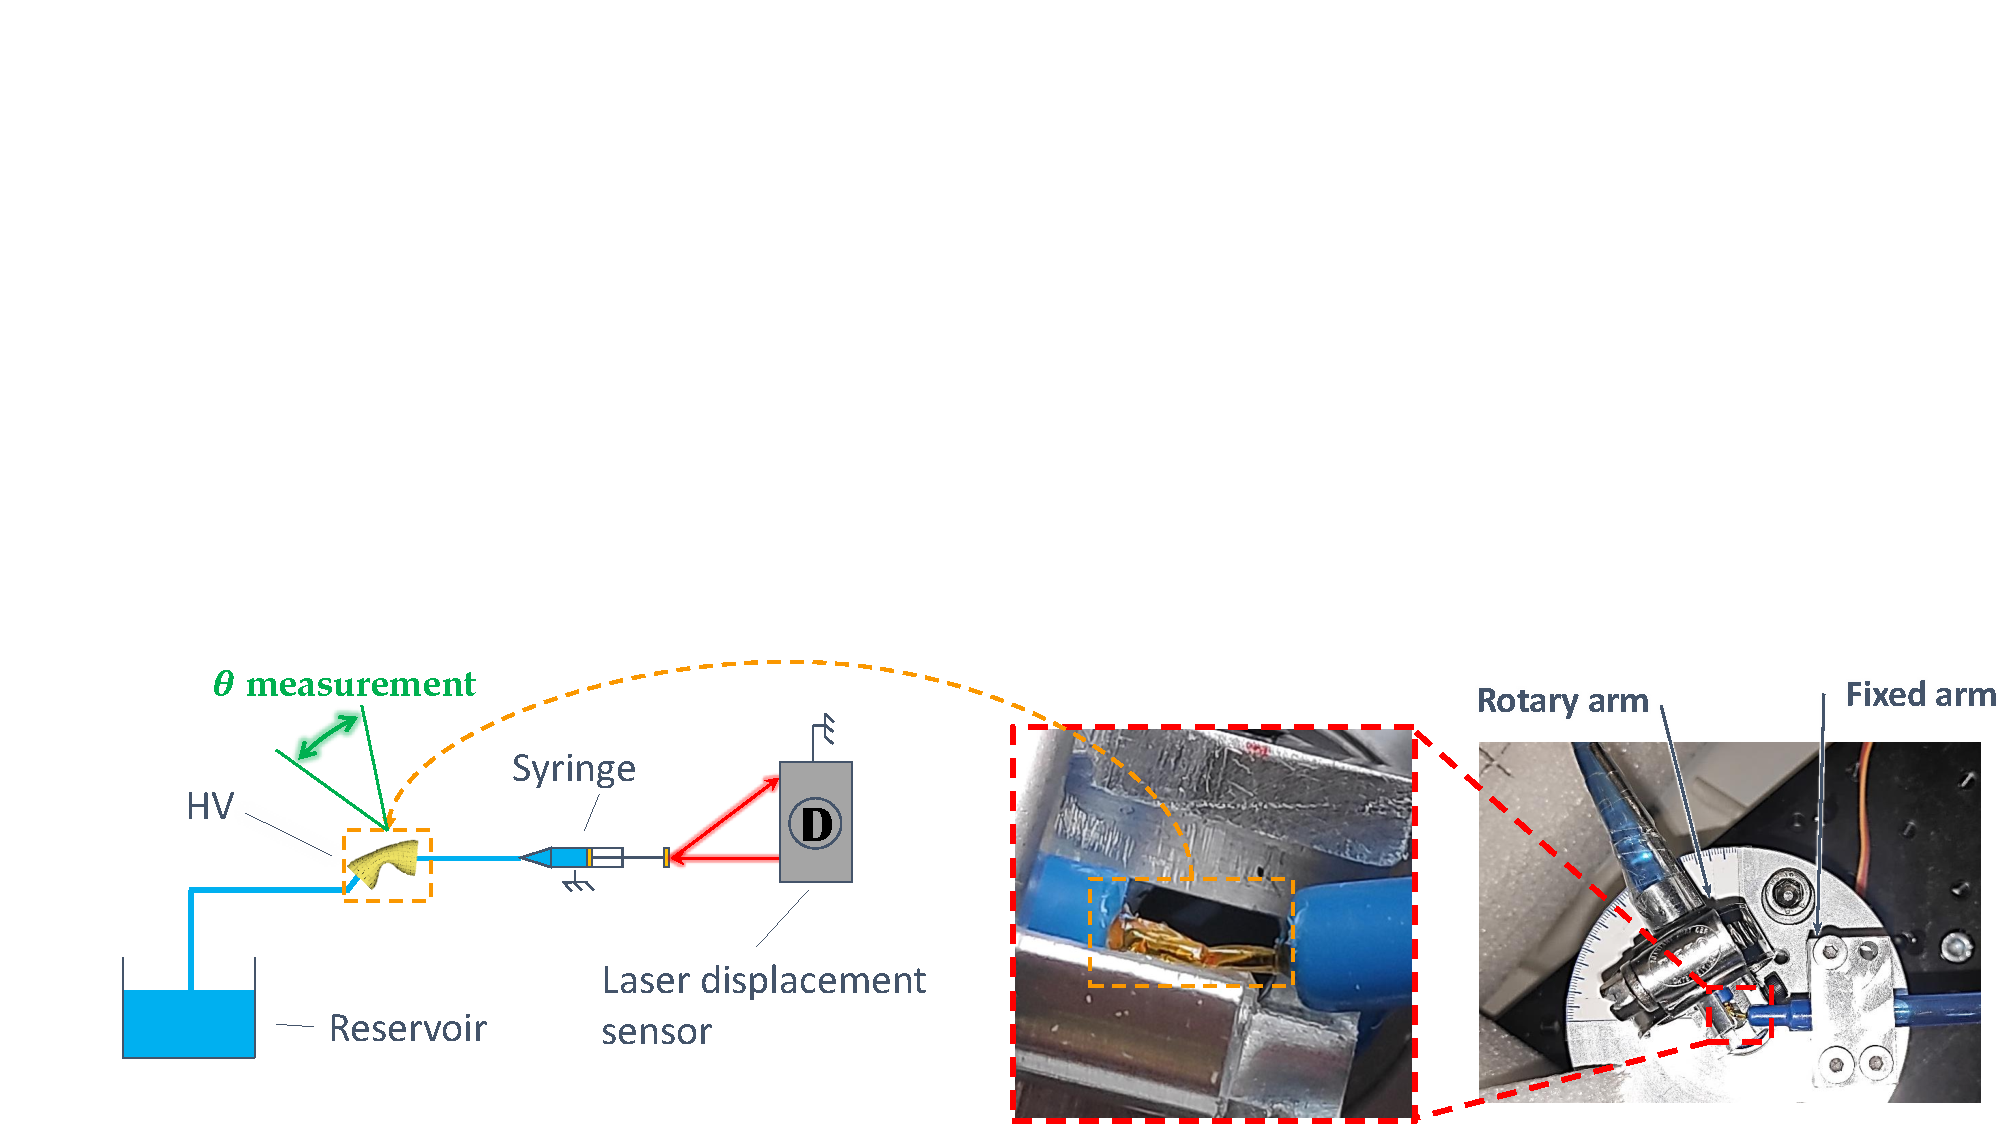
\includegraphics[trim={2cm 0cm 0cm 10cm},clip,width=\textwidth]{figures/essais_hydraulique_VH.pdf}
	\caption{Essais de caractérisations hydrauliques de VH}
	\label{fig:essais_hydraulique_VH}
\end{center}	
\end{figure*}    
%%%%%%%%%%%%%%%%%%%%%%%%%%%%%%%%%%%%  
%%%%%%%%%%%%%%%%%%%%%%%%%%%%%%%%%%%%	
\begin{figure}[!htb]
\begin{center}
	\captionsetup{justification=centering} 
	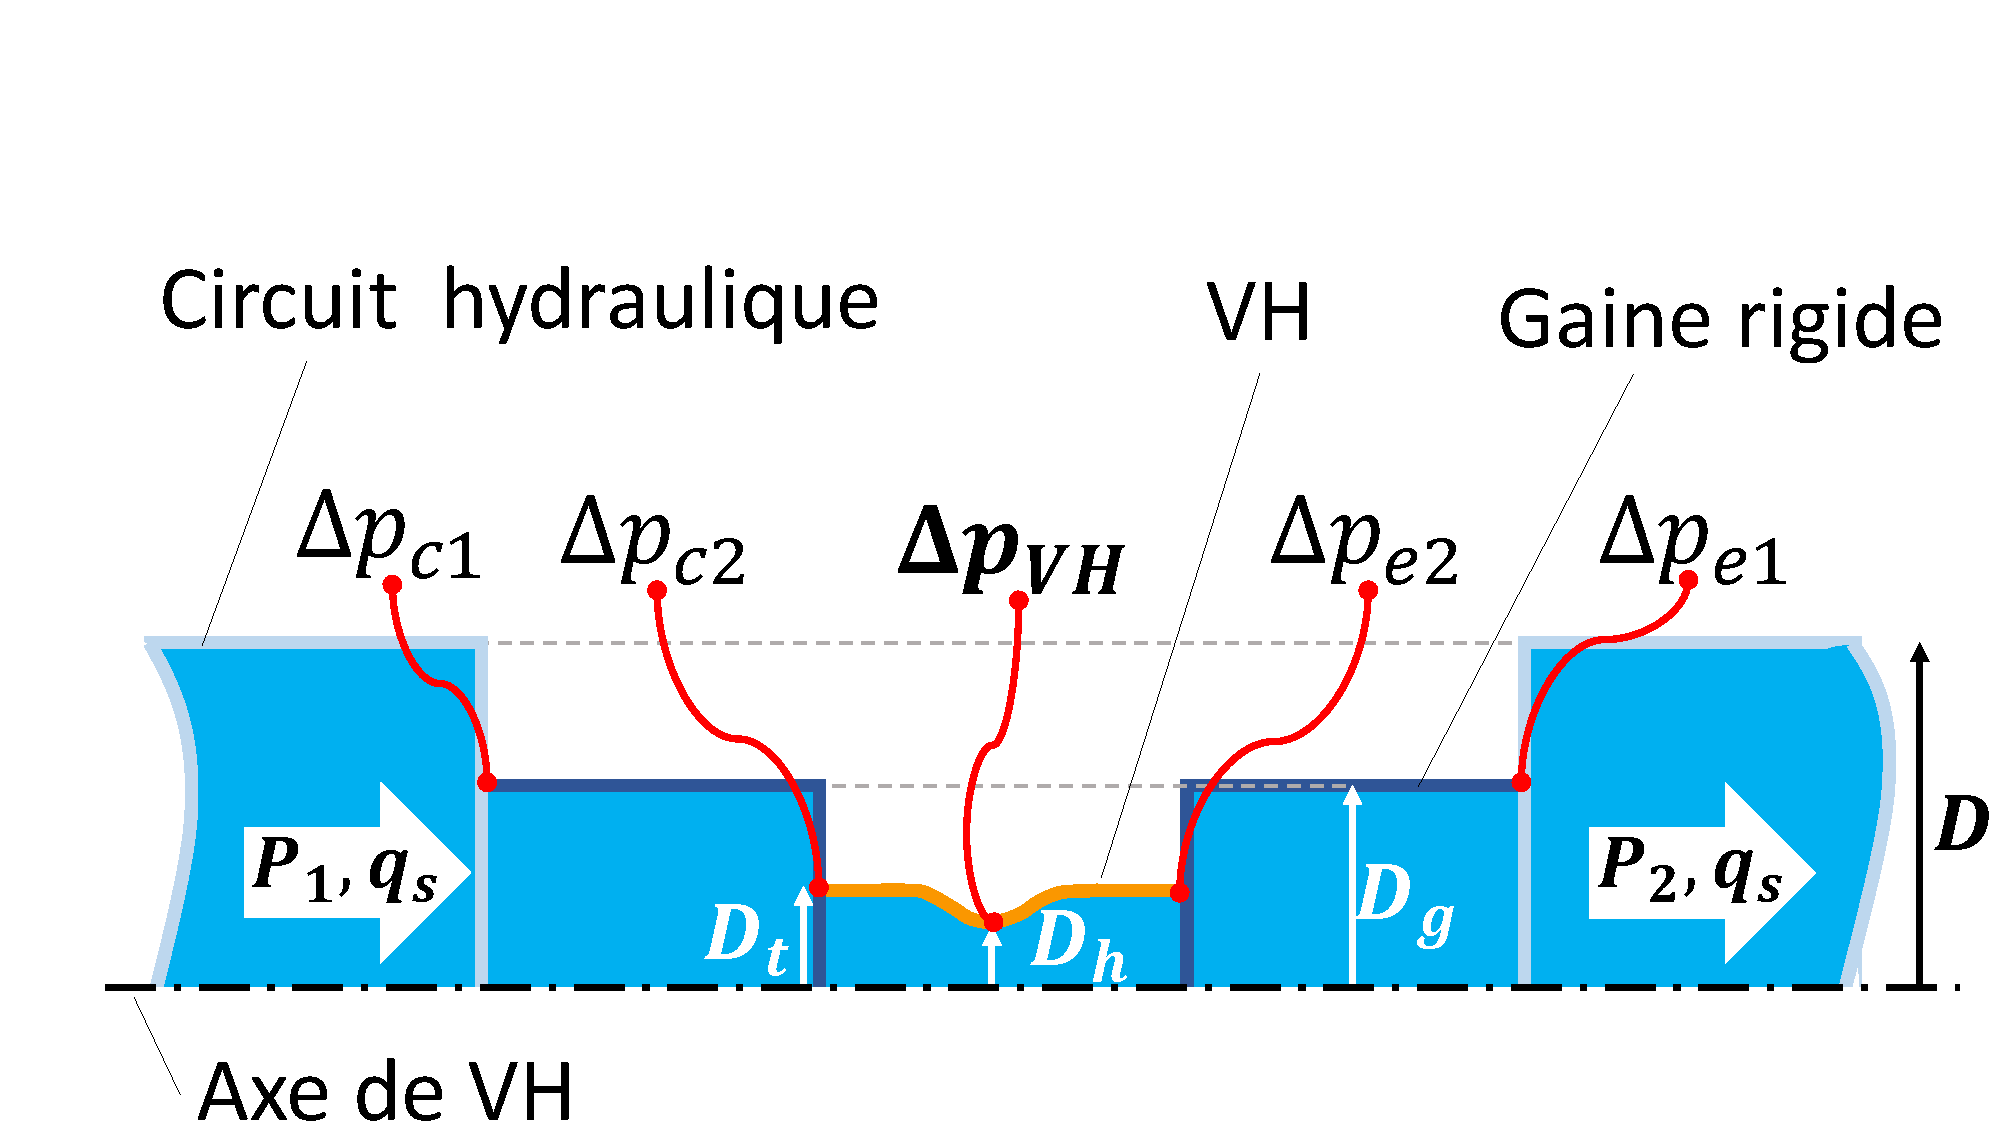
\includegraphics[trim={2cm 0cm 0cm 4cm},clip,width=0.49\textwidth]{figures/fabrication_tube_experimental.pdf}
	\caption{Méthode de fabrication de la VH}
	\label{fig:fabrication_tube_experimental}
\end{center}	
\end{figure}    
%%%%%%%%%%%%%%%%%%%%%%%%%%%%%%%%%%%% 
%%%%%%%%%%%%%%%%%%%%%%%%%
\begin{figure}[!htbp]
\begin{center}
	\captionsetup{justification=centering}
	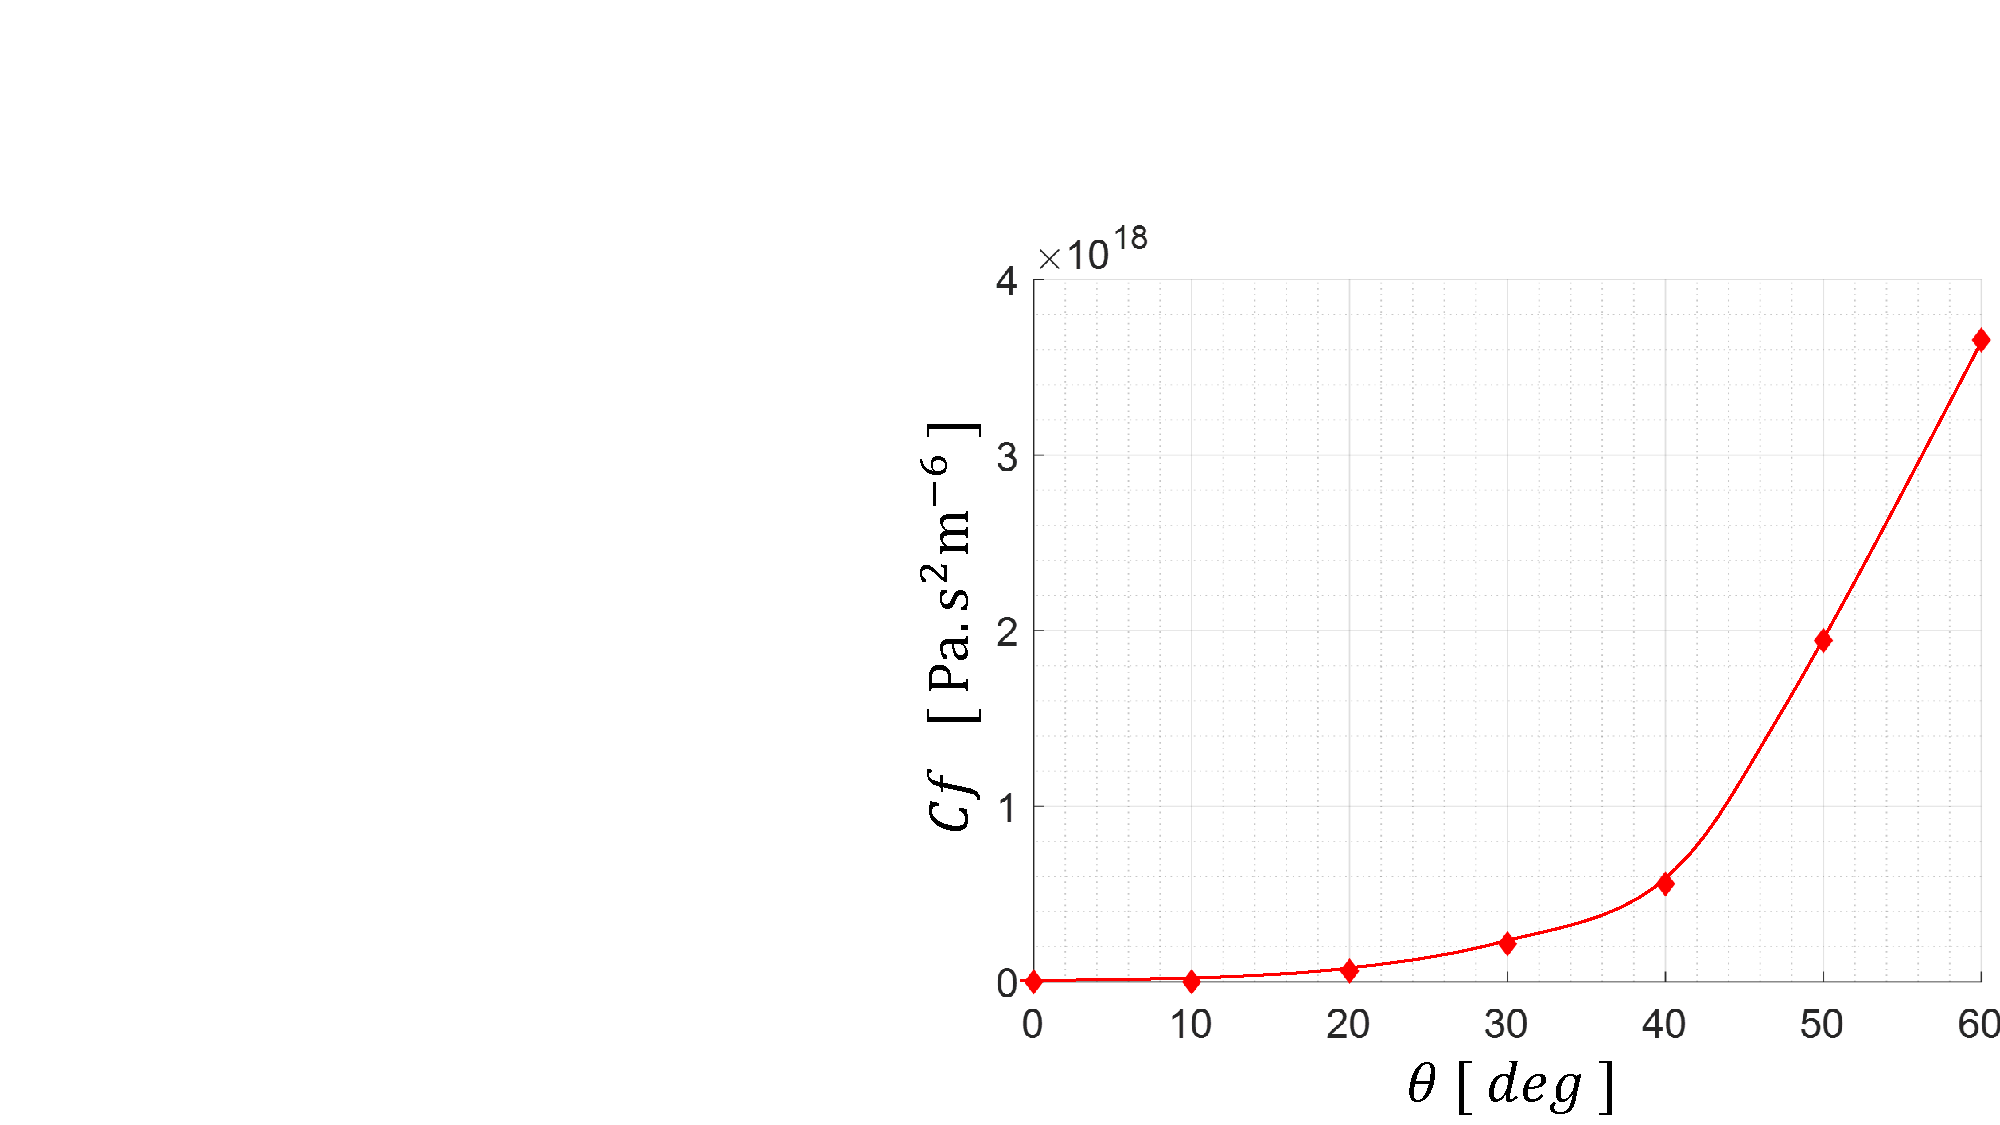
\includegraphics[trim={10cm 0cm 0cm 0cm},clip,width=0.49\textwidth]{figures/resultats_essais_hydraulique_VH_D1mm.pdf}
	\caption{$Cf_{VH}$ calculé à partir des essais pour 7 incréments d'angles}
	\label{fig:resultats_essais_hydraulique_VH_D1mm}
\end{center}
\end{figure}
%%%%%%%%%%%%%%%%
	%/////////////////////////////////////////////
	\subsection{The HV mechanical influence on the electromechanical converter (théorique = x0 réduit donc faut compenser)}	
	\label{The mechanical influence of the valve on the electromechanical converter}
	%/////////////////////////////////////////////
Theoretically...

%/!\/!\/!\/!\/!\/!\/!\/!\/!\/!\/!\/!\/!\/!\/!\/!\/!\/!\/!\/!\/!\/!\/!\/!\%
\section{MODEL RECALIBRATION WITH EXPERIMENTAL DATA}
\label{sec:MODEL RECALIBRATION WITH EXPERIMENTAL DATA}
%/!\/!\/!\/!\/!\/!\/!\/!\/!\/!\/!\/!\/!\/!\/!\/!\/!\/!\/!\/!\/!\/!\/!\/!\%
	%/////////////////////////////////////////////
	\subsubsection{Free release trials}
	%/////////////////////////////////////////////

%%%%%%%%%%%%%%%%%%%%%%%%%%%%%%%%%%%%	
\begin{figure}[!htbp]
	\begin{center}
		\captionsetup{justification=centering}
		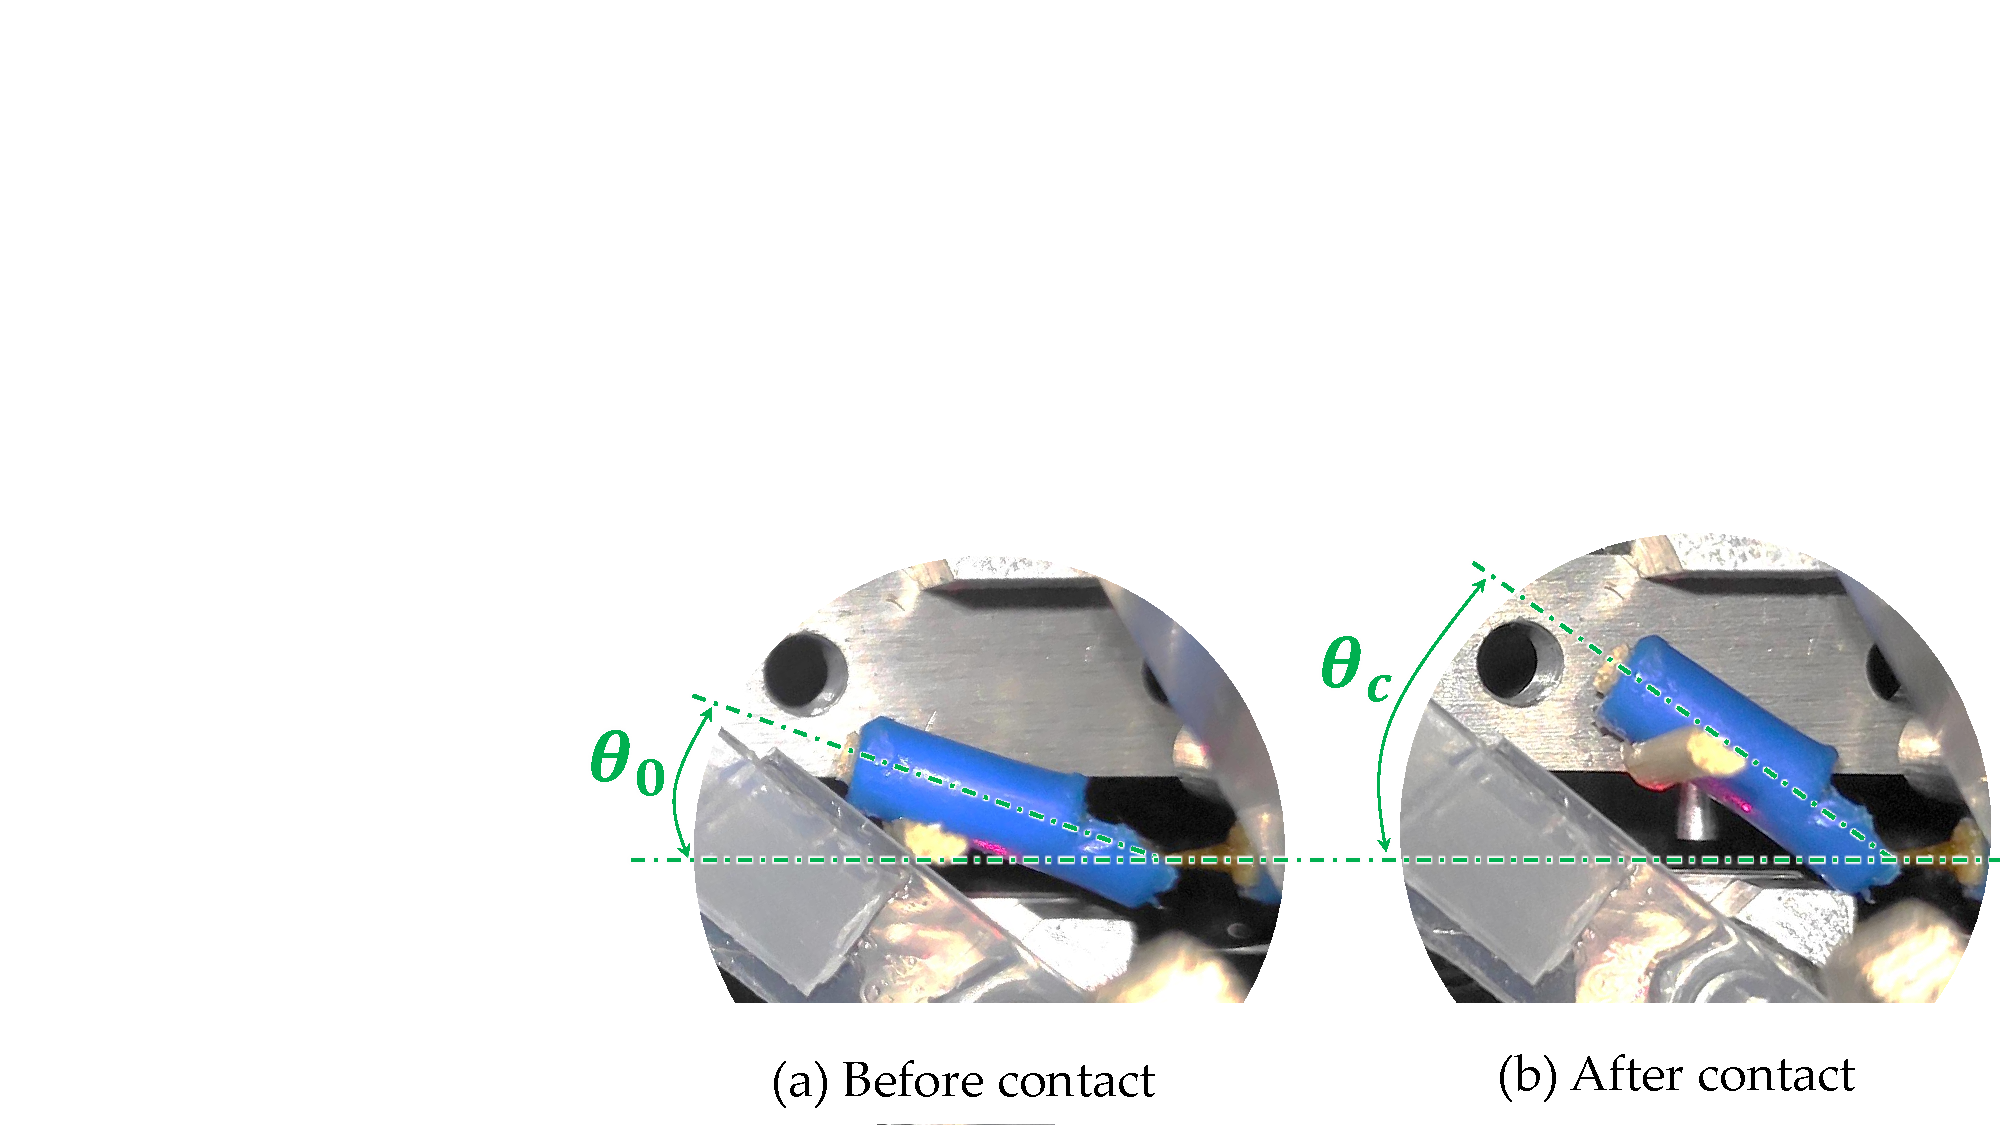
\includegraphics[trim={4cm 0cm 0cm 9.5cm},clip,width=0.7\textwidth]{figures/contact_M_VH_lachers.pdf}
		\caption{Image de la VH$_{T100p}$ lorsque $\theta_0$($x_m=-x_{0})$ et lorsque $\theta_f$($x_m=x_{0,vh}$)}
		\label{fig:contact_M_VH_lachers}
	\end{center}
\end{figure}
%%%%%%%%%%%%%%%%%%%%%%%%%%%%%%%%%%%%

	%/////////////////////////////////////////////
	\subsubsection{Recalibrated model}
	%/////////////////////////////////////////////

%%%%%%%%%%%%%%%%%%%%%%%%%%%%%%%%%%%
\begin{table}[!htbp]
	\centering
	% \resizebox{\textwidth}{!}{%
		\begin{tabular}[t]{c|c|c}
\toprule
\multicolumn{1}{c}{\textbf{Parameter}}	&
\multicolumn{1}{c}{\textbf{Value OB}} 	& 
\multicolumn{1}{c}{\textbf{Value OBVH}}  \\
\midrule
$D_g$ [mm] 						& \cellcolor{ashgrey} 		& \textcolor{red}{4} 		\\ \hline
$\Delta\theta$ [deg] 			& \cellcolor{ashgrey} 		& \textcolor{red}{{[$\approx$ 19 ; $\approx$ 36]}} \\ \hline
$K_{T100p}(\theta_f)$ [Nmm/rad] & \cellcolor{ashgrey}  		&  0.27 					\\ \hline
$a$ [mm]         			    & \cellcolor{ashgrey}  		&  2.24				 	 	\\ \hline
$\mu_{fs}$ [~~] 				& \cellcolor{ashgrey}  		&  0.42  					\\ \hline
$K$ [N/m] 						&	84480			  	 	&  84480  					\\ \hline
$x_0$ [mm] 						& \textcolor{red}{0.59}		& \textcolor{red}{0.50}  	\\ \hline
$v_0$ [mm/s] 					& \textcolor{red}{10}		& \textcolor{red}{65}  		\\ \hline
$Q$	[~~] 						& 		24.0		 		& 5.0     					\\ \hline
$k^2_{sys}$ [\%] 				& 		1.25		 		& \textcolor{red}{1.25}   	\\ \hline
$\eta_{ob}$ [\%] 				& 		11.9		 		& 2.6   					\\ \hline	
$R_{ch}$ [k$\text{\ohm}$] 		&	\textcolor{red}{15.5}	& \textcolor{red}{15.5}    	\\ \hline		
$m$	[g]						    &	\textcolor{red}{5.88}	& 9.00   					\\ \hline	
$f_0$ [Hz]						&		32.9				& 27.9   					\\
\bottomrule	
	\end{tabular}
        \caption{Value des paramètres de l'OB et de l'ensemble OBVH implémentant le tube T100p suite au essais de lâchers expérimentaux}
        \label{tab:parametres lacher tube}
\end{table}        
%%%%%%%%%%%%%%%%%%%%%%%%%%%%%%%%%%%%

%/!\/!\/!\/!\/!\/!\/!\/!\/!\/!\/!\/!\/!\/!\/!\/!\/!\/!\/!\/!\/!\/!\/!\/!\%
\section{ANALYZE AND DISCUSSION}
\label{sec:ANALYZE AND DISCUSSION}
%/!\/!\/!\/!\/!\/!\/!\/!\/!\/!\/!\/!\/!\/!\/!\/!\/!\/!\/!\/!\/!\/!\/!\/!\%

%/!\/!\/!\/!\/!\/!\/!\/!\/!\/!\/!\/!\/!\/!\/!\/!\/!\/!\/!\/!\/!\/!\/!\/!\%
\section{CONCLUSION}
\label{sec:CONCLUSION}
%/!\/!\/!\/!\/!\/!\/!\/!\/!\/!\/!\/!\/!\/!\/!\/!\/!\/!\/!\/!\/!\/!\/!\/!\%


%% If you have bibdatabase file and want bibtex to generate the
%% bibitems, please use
%%
%%  \bibliographystyle{elsarticle-num} 
%%  \bibliography{<your bibdatabase>}

%% else use the following coding to input the bibitems directly in the
%% TeX file.

%\begin{thebibliography}{00}
\bibliography{biblioArticle1.bib}
\bibliographystyle{elsarticle-num}
%\bibliographystyle{unsrt} 
%\end{thebibliography}


\end{document}
\endinput